\documentclass[a4paper,oneside]{report}

% ==========================================
% 1. CẤU HÌNH NGÔN NGỮ, PHÔNG CHỮ & KÍCH THƯỚC
% ==========================================
\usepackage[utf8]{inputenc}
\usepackage{newunicodechar}
\newunicodechar{μ}{\ensuremath{\mu}}
\usepackage[T5]{fontenc}
\usepackage[vietnamese]{babel}
\usepackage{times}
\usepackage{fontsize}
\changefontsize{13pt}

\usepackage{setspace}
\onehalfspacing

\usepackage{geometry}
\geometry{
    a4paper,
    top=25mm,
    bottom=25mm,
    left=30mm,
    right=20mm
}

\usepackage{indentfirst}
\setlength{\parindent}{1.27cm}
\setlength{\parskip}{6pt}

% ==========================================
% 2. ĐỒ HỌA, BẢNG BIỂU, CODE, LINK
% ==========================================
\usepackage{amsmath,amsfonts,amssymb}
\usepackage{tikz}
\usetikzlibrary{fit}
\usepackage{tikz-cd}
\usepackage{multicol}

\usepackage{graphicx}
\usepackage{float}
\usepackage{caption}
\usepackage{subcaption}
\usepackage{placeins}
\graphicspath{{images/}}

\usepackage{booktabs}
\usepackage{tabularx}
\usepackage{longtable}
\usepackage{multirow}
\usepackage{array}
\usepackage{makecell}

\usepackage{listings}
\usepackage{xcolor}

\usepackage{enumitem}
\usepackage{xurl}
\usepackage[noprefix]{nomencl}
\makenomenclature

\usepackage{titletoc}
\usepackage{titlesec}

\newcommand{\conclusionsection}[1]{%
    \vspace{1em}
    {\large\bfseries #1\par}
    \vspace{0.5em}
}

\newcommand{\conclusionsubsection}[1]{%
    \vspace{0.7em}
    {\normalsize\bfseries #1\par}
    \vspace{0.3em}
}

% ==========================================
% TÀI LIỆU THAM KHẢO
% ==========================================
\usepackage[
    backend=biber,
    style=ieee,
    sorting=none
]{biblatex}
% Vietnamese strings come from report/vietnamese.lbx (biblatex has none).

\addbibresource{reference.bib}

\usepackage{hyperref}
\hypersetup{
    colorlinks=true,
    linkcolor=black,
    filecolor=magenta,
    urlcolor=blue,
    citecolor=black
}

% ==========================================
% 3. TÊN HIỂN THỊ, MỤC LỤC & DANH MỤC
% ==========================================
\addto\captionsvietnamese{
  \renewcommand{\contentsname}{MỤC LỤC}
  \renewcommand{\listtablename}{DANH MỤC BẢNG}
  \renewcommand{\listfigurename}{DANH MỤC HÌNH VẼ}
  \renewcommand{\bibname}{TÀI LIỆU THAM KHẢO}
}

\renewcommand{\nomname}{DANH MỤC THUẬT NGỮ VIẾT TẮT}

\titlecontents{chapter}
  [0pt]
  {\vspace{0.5em}\bfseries}
  {CHƯƠNG \thecontentslabel:\quad}
  {}
  {\titlerule*[0.5pc]{.}\contentspage}

\setcounter{secnumdepth}{3}
\setcounter{tocdepth}{2}

% ==========================================
% 4. ĐỊNH DẠNG TIÊU ĐỀ
% ==========================================
\titleformat{\chapter}[block]
  {\normalfont\fontfamily{ptm}\fontsize{16pt}{20pt}\selectfont\bfseries\centering}
  {CHƯƠNG \thechapter.\ }
  {0pt}
  {\MakeUppercase}

\titlespacing*{\chapter}{0pt}{-20pt}{24pt}

\titleformat{\section}
  {\normalfont\fontfamily{ptm}\fontsize{13pt}{\baselineskip}\selectfont\bfseries}
  {\thesection\quad}
  {0pt}
  {}

\titleformat{\subsection}
  {\normalfont\fontfamily{ptm}\fontsize{13pt}{\baselineskip}\selectfont\bfseries}
  {\thesubsection\quad}
  {0pt}
  {}

\renewcommand{\thesubsubsection}{\alph{subsubsection}}

\titleformat{\subsubsection}
  {\normalfont\fontfamily{ptm}\fontsize{13pt}{\baselineskip}\selectfont\bfseries}
  {\thesubsubsection)\quad}
  {0pt}
  {}

% ==========================================
% 5. DANH SÁCH
% ==========================================
\setlist[itemize,1]{
    label={-},
    leftmargin=1.8cm,
    itemindent=0pt,
    labelsep=0.5em,
    topsep=0pt,
    itemsep=0pt
}

% ==========================================
% 6. CODE LISTING
% ==========================================
\lstdefinestyle{terminal}{
    basicstyle=\ttfamily\footnotesize,
    backgroundcolor=\color{black!90},
    keywordstyle=\color{green!70},
    stringstyle=\color{yellow},
    commentstyle=\color{gray},
    frame=single,
    rulecolor=\color{black},
    breaklines=true,
    showstringspaces=false,
    xleftmargin=6pt,
    xrightmargin=6pt,
    framesep=4pt
}

\lstdefinestyle{codestyle}{
    basicstyle=\ttfamily\small,
    keywordstyle=\bfseries\color{blue!70!black},
    commentstyle=\itshape\color{gray},
    stringstyle=\color{orange!80!black},
    backgroundcolor=\color{gray!8},
    frame=single,
    rulecolor=\color{gray!40},
    breaklines=true,
    showstringspaces=false,
    numbers=left,
    numberstyle=\tiny\color{gray},
    numbersep=6pt,
    xleftmargin=12pt,
    captionpos=b
}

% ==========================================
% 7. MACRO TỰ ĐỊNH NGHĨA
% ==========================================
\newcommand{\todofigure}[3]{%
\begin{figure}[h]
    \centering
    \fbox{
        \begin{minipage}[c][0.22\textheight][c]{0.82\textwidth}
            \centering
            \textbf{TODO: Bổ sung hình minh họa}\\[0.5em]
            \texttt{\detokenize{#1}}
        \end{minipage}
    }
    \caption{#2}
    \label{#3}
\end{figure}
}

% ------------------------------------------
% Bổ sung cho báo cáo này
% ------------------------------------------
\usepackage{fancyvrb}
\usetikzlibrary{shapes.multipart,positioning,arrows.meta,calc}
\graphicspath{{figures/images/}}

% Đoạn mã SQL (chỉ chứa ký tự ASCII: listings không xử lý được UTF-8 nhiều byte).
\lstdefinelanguage{TSQL}[]{SQL}{
    morekeywords={GO,TOP,PERCENT,OUTPUT,THROW,TRY,CATCH,TRANSACTION,ROLLBACK,COMMIT,
        EXECUTE,EXEC,REVERT,NOCOUNT,PERSISTED,SCHEMABINDING,RETURNS,RETURN,CROSS,APPLY,
        OPENJSON,STRING_AGG,STRING_SPLIT,TRANSLATE,WITHIN,OVER,PARTITION,ROW_NUMBER,RANK,
        MERGE,IDENTITY,NVARCHAR,VARCHAR,DECIMAL,DATETIME2,BIT,TINYINT,SMALLINT,BIGINT,
        INTERSECT,EXCEPT,FULL,OUTER,RIGHT,LEFT,COLLATE,SESSION_CONTEXT,IF,ELSE,BEGIN,END,
        DECLARE,SET,PROCEDURE,FUNCTION,TRIGGER,VIEW,AFTER,ROLE,USER,LOGIN,WITHOUT,REVERT,
        CHECK,OPTION,CONSTRAINT,REFERENCES,CASCADE,DEFAULT,UNIQUE,PRIMARY,FOREIGN,KEY,
        SCOPE_IDENTITY,XACT_ABORT,COALESCE,LOG,CONCAT,CAST}
}
\lstset{style=codestyle, language=TSQL, basicstyle=\ttfamily\footnotesize}

% Thực thể trong sơ đồ ERD: tên ở phần trên, thuộc tính ở phần dưới.
\tikzset{
    entity/.style={rectangle split, rectangle split parts=2, draw=blue!60!black, thick,
        rounded corners=2pt, rectangle split part fill={blue!12, white},
        font=\scriptsize, align=left, inner sep=3pt},
    refentity/.style={entity, draw=gray, dashed, rectangle split part fill={gray!15, white}},
    rel/.style={draw=black!70, thick},
    card/.style={font=\scriptsize\bfseries, fill=white, inner sep=1pt},
}
\newcommand{\pk}[1]{\underline{#1}}
\newcommand{\attrs}[1]{\begin{tabular}{@{}l@{}}#1\end{tabular}}

\begin{document}
% Cho phép xuống dòng sau dấu _ trong tên bảng/cột, và giãn khoảng trắng
% thay vì để chữ tràn lề.
\DeclareRobustCommand{\_}{\textunderscore\allowbreak}
\sloppy

% ------------------------------------------
% PHẦN TRƯỚC NỘI DUNG
% ------------------------------------------
\pagenumbering{roman}
\setcounter{page}{1}

% --- TRANG BÌA ---
\begin{titlepage}
\thispagestyle{empty}
\begin{tikzpicture}[remember picture,overlay]
\draw[line width=2pt,blue!70!black]
([xshift=3cm,yshift=-2.5cm]current page.north west)
rectangle
([xshift=-2cm,yshift=2.5cm]current page.south east);
\draw[line width=0.6pt,blue!70!black]
([xshift=3.15cm,yshift=-2.65cm]current page.north west)
rectangle
([xshift=-2.15cm,yshift=2.65cm]current page.south east);
\end{tikzpicture}
\begin{center}
\vspace*{0.25cm}
{\fontsize{18pt}{22pt}\selectfont\bfseries
BỘ KHOA HỌC VÀ CÔNG NGHỆ\par}
\vspace{0.35cm}
{\fontsize{16pt}{20pt}\selectfont\bfseries
HỌC VIỆN CÔNG NGHỆ BƯU CHÍNH VIỄN THÔNG\par}\vspace{-0.15cm}
\rule{5.4cm}{0.5pt}

\vspace{1.2cm}

\includegraphics[width=0.3\linewidth]{figures/images/logoptit1.png}

\vspace{1.3cm}
{\bfseries BÁO CÁO BÀI TẬP LỚN\par}
\vspace{0.2cm}
{\bfseries MÔN HỆ QUẢN TRỊ CƠ SỞ DỮ LIỆU\par}
\vspace{0.45cm}
\begin{minipage}{0.84\textwidth}
\centering
{\bfseries ĐỀ TÀI \\
THIẾT KẾ VÀ TRIỂN KHAI CƠ SỞ DỮ LIỆU CHO THƯ VIỆN SỐ TƯ LIỆU NGHE NHÌN TRÊN SQL SERVER}
\end{minipage}

\vspace{1.1cm}
\begin{tabular}{>{\bfseries}r@{\hspace{0.8cm}}p{9.5cm}}
Giảng viên hướng dẫn: & Vũ Tiến Tài \\
\addlinespace[0.3cm]
Lớp / nhóm: & INT14168 -- Nhóm 4 \\
\addlinespace[0.3cm]
Sinh viên thực hiện:
& Hoàng Đinh Tuấn Anh -- B24DCKD003 \\
\addlinespace[0.15cm]
& Phạm Đức Minh -- B24DCKD056 \\
\addlinespace[0.15cm]
& Phan Nguyễn Trung Khánh -- B24DCKD041 \\
\addlinespace[0.15cm]
& Nguyễn Đức Vũ -- B24DCKD013 \\
\addlinespace[0.15cm]
& Nguyễn Đăng Minh -- B24DCKD055 \\
\end{tabular}

\vfill
{\bfseries Hà Nội - 2026}\par
\vspace*{0.75cm}
\end{center}
\end{titlepage}


% --- NHẬN XÉT, ĐÁNH GIÁ, CHO ĐIỂM ---
\clearpage
\thispagestyle{empty}

\begin{center}
\vspace*{0.8cm}
{\bfseries NHẬN XÉT, ĐÁNH GIÁ, CHO ĐIỂM\par}
\vspace{0.25cm}
{\bfseries (của giảng viên)\par}
\end{center}

\vspace{0.5cm}

\noindent\makebox[\textwidth]{\dotfill}\par\vspace{0.35cm}
\noindent\makebox[\textwidth]{\dotfill}\par\vspace{0.35cm}
\noindent\makebox[\textwidth]{\dotfill}\par\vspace{0.35cm}
\noindent\makebox[\textwidth]{\dotfill}\par\vspace{0.35cm}
\noindent\makebox[\textwidth]{\dotfill}\par\vspace{0.35cm}
\noindent\makebox[\textwidth]{\dotfill}\par\vspace{0.35cm}
\noindent\makebox[\textwidth]{\dotfill}\par\vspace{0.35cm}
\noindent\makebox[\textwidth]{\dotfill}\par\vspace{0.35cm}
\noindent\makebox[\textwidth]{\dotfill}\par\vspace{0.35cm}
\noindent\makebox[\textwidth]{\dotfill}\par\vspace{0.35cm}
\vspace{1cm}

\noindent
\textbf{Điểm:} \makebox[4.2cm]{\dotfill}
\textit{(Bằng chữ:}\makebox[4.5cm]{\dotfill}\textit{)}

\vspace{1cm}

\begin{flushright}
Hà Nội, Ngày \makebox[0.8cm]{\dotfill}
Tháng \makebox[0.8cm]{\dotfill}
Năm 2026

\vspace{0.2cm}

\textbf{GIẢNG VIÊN}

\vspace{0.3cm}

\textit{(ký, họ tên)}
\end{flushright}

\newpage

\clearpage\chapter*{LỜI NÓI ĐẦU}
\addcontentsline{toc}{chapter}{LỜI NÓI ĐẦU}

Đài truyền hình, toà báo, trường đại học và bảo tàng đều đang giữ những kho video lớn,
nhưng mỗi kho nằm riêng ở một đơn vị và gần như chỉ được ghi tên chương trình, ngày phát hành.
Một nhà báo, nhà nghiên cứu hay sinh viên cần một đoạn tư liệu cũ, như một khoảnh khắc trên
đường đua, một dòng chữ trên bảng điểm hay một câu bình luận, thường không biết nó nằm ở đâu,
và khi tìm ra thì còn phải xin phép đơn vị giữ bản quyền. Một thư viện số dùng chung giải
quyết cả hai việc. Nó cần một cơ sở dữ liệu lưu được danh mục của nhiều đơn vị cùng hàng
nghìn khung hình kèm văn bản trích từ hình và lời nói, quản lý yêu cầu khai thác và giấy phép
sử dụng, tài khoản của nhiều loại người dùng và nhật ký thao tác. Đồng thời nó phải bảo đảm
tính toàn vẹn và phân quyền.

Báo cáo này trình bày việc thiết kế và triển khai cơ sở dữ liệu cho một hệ thống như vậy trên
Microsoft SQL Server (bản Express), theo một tình huống giả định: \textit{thư viện số tư
liệu nghe nhìn} dùng chung cho nhiều đơn vị. Toàn bộ dữ liệu, chỉ mục văn bản, việc gộp kết
quả tìm kiếm, quy trình yêu cầu khai thác và cấp phép, tài khoản và phân quyền được hiện thực
bằng T-SQL: bảng có đầy đủ ràng buộc được đặt tên, hàm, thủ tục lưu trữ, view, trigger và phân
quyền mức cơ sở dữ liệu. Một ứng dụng web nhỏ dùng chính cơ sở dữ liệu này để bạn đọc tra cứu
và gửi yêu cầu, còn cán bộ thư viện chọn đoạn tư liệu và cấp phép. Video mẫu là 25 đoạn tường
thuật giải đua xe đạp tiếng Việt lấy từ một bộ dữ liệu video công khai; danh mục các đơn vị
và giấy phép quanh đó là dữ liệu minh hoạ.

Nội dung báo cáo gồm ba chương. Chương 1 khảo sát bài toán và phân tích yêu cầu. Chương 2
trình bày thiết kế cơ sở dữ liệu: thực thể, sơ đồ ERD, quá trình chuẩn hoá đến dạng chuẩn 3,
dư thừa có kiểm soát, danh sách bảng và ràng buộc. Chương 3 trình bày cài đặt các đối tượng T-SQL, các truy vấn
nghiệp vụ, kiểm thử, ứng dụng minh hoạ và kết quả đo chất lượng tìm kiếm.

Do thời gian và kiến thức còn hạn chế, báo cáo khó tránh khỏi thiếu sót. Nhóm rất mong
nhận được góp ý của thầy/cô để đề tài được hoàn thiện hơn.
\\
\vfill

\begin{flushright}
\textit{Hà Nội, năm 2026}\\
\textbf{Nhóm sinh viên thực hiện}
\end{flushright}

\newpage

\chapter*{LỜI CẢM ƠN}
\addcontentsline{toc}{chapter}{LỜI CẢM ƠN}

% [Nhóm tự hoàn thiện đoạn cảm ơn theo ý mình.]
Nhóm xin chân thành cảm ơn [học hàm, học vị, họ tên giảng viên] đã giảng dạy học phần Hệ
quản trị cơ sở dữ liệu và hướng dẫn nhóm trong quá trình thực hiện bài tập lớn. Những kiến
thức về mô hình dữ liệu quan hệ, chuẩn hoá, ràng buộc toàn vẹn, thủ tục lưu trữ, giao dịch và
phân quyền là nền tảng để nhóm thiết kế và triển khai hệ thống trong báo cáo này.

Nhóm cũng cảm ơn các tác giả của bộ dữ liệu video công khai và của các mô hình, thư viện mã
nguồn mở (SigLIP2, FAISS) được sử dụng trong đề tài.

Mặc dù đã cố gắng, báo cáo chắc chắn còn những thiếu sót. Nhóm rất mong nhận được góp ý
của thầy/cô.

\begin{flushright}
\textbf{Nhóm sinh viên thực hiện}
\end{flushright}
\clearpage

\newpage

\chapter*{DANH MỤC TỪ VIẾT TẮT}
\addcontentsline{toc}{chapter}{DANH MỤC TỪ VIẾT TẮT}

\renewcommand{\arraystretch}{1.25}
\begin{longtable}{
    >{\raggedright\arraybackslash}p{0.16\textwidth}
    >{\raggedright\arraybackslash}p{0.38\textwidth}
    >{\raggedright\arraybackslash}p{0.36\textwidth}
}
\toprule
\textbf{Từ viết tắt} & \textbf{Tiếng Anh} & \textbf{Tiếng Việt} \\
\midrule
\endfirsthead
\toprule
\textbf{Từ viết tắt} & \textbf{Tiếng Anh} & \textbf{Tiếng Việt} \\
\midrule
\endhead
\bottomrule
\endfoot

1NF, 2NF, 3NF & First/Second/Third Normal Form & Dạng chuẩn 1, 2, 3 \\
ASR & Automatic Speech Recognition & Nhận dạng tiếng nói tự động \\
BCNF & Boyce--Codd Normal Form & Dạng chuẩn Boyce--Codd \\
CK & Check constraint & Ràng buộc kiểm tra \\
CPU & Central Processing Unit & Bộ xử lý trung tâm \\
CSDL & -- & Cơ sở dữ liệu \\
CSV & Comma-Separated Values & Tệp giá trị phân tách bằng dấu phẩy \\
CTE & Common Table Expression & Biểu thức bảng dùng chung \\
DBMS & Database Management System & Hệ quản trị cơ sở dữ liệu \\
DDL & Data Definition Language & Ngôn ngữ định nghĩa dữ liệu \\
DF & Default constraint & Ràng buộc giá trị mặc định \\
DML & Data Manipulation Language & Ngôn ngữ thao tác dữ liệu \\
ERD & Entity--Relationship Diagram & Sơ đồ thực thể -- liên kết \\
FAISS & Facebook AI Similarity Search & Thư viện tìm kiếm vector tương tự \\
FK & Foreign Key & Khoá ngoại \\
IDF & Inverse Document Frequency & Tần suất tài liệu nghịch đảo \\
JSON & JavaScript Object Notation & Định dạng dữ liệu JSON \\
MRR & Mean Reciprocal Rank & Trung bình nghịch đảo thứ hạng \\
OCR & Optical Character Recognition & Nhận dạng ký tự quang học \\
ODBC & Open Database Connectivity & Giao diện kết nối cơ sở dữ liệu mở \\
PK & Primary Key & Khoá chính \\
R@K & Recall at K & Tỉ lệ tìm thấy trong K kết quả đầu \\
RBAC & Role-Based Access Control & Phân quyền theo vai trò \\
RRF & Reciprocal Rank Fusion & Gộp xếp hạng theo nghịch đảo thứ hạng \\
SQL & Structured Query Language & Ngôn ngữ truy vấn có cấu trúc \\
SSMS & SQL Server Management Studio & Công cụ quản trị SQL Server \\
T-SQL & Transact-SQL & Phương ngữ SQL của SQL Server \\
TVF & Table-Valued Function & Hàm trả về bảng \\
UDF & User-Defined Function & Hàm do người dùng định nghĩa \\
UQ & Unique constraint & Ràng buộc duy nhất \\
\end{longtable}

\newpage

\chapter*{DANH MỤC THUẬT NGỮ}
\addcontentsline{toc}{chapter}{DANH MỤC THUẬT NGỮ}

\renewcommand{\arraystretch}{1.25}
\begin{longtable}{
    >{\raggedright\arraybackslash}p{0.26\textwidth}
    >{\raggedright\arraybackslash}p{0.26\textwidth}
    >{\raggedright\arraybackslash}p{0.38\textwidth}
}
\toprule
\textbf{Thuật ngữ tiếng Anh} & \textbf{Tiếng Việt} & \textbf{Giải thích ngắn} \\
\midrule
\endfirsthead
\toprule
\textbf{Thuật ngữ tiếng Anh} & \textbf{Tiếng Việt} & \textbf{Giải thích ngắn} \\
\midrule
\endhead
\bottomrule
\endfoot

Candidate key & Khoá ứng viên & Tập thuộc tính tối thiểu xác định duy nhất một dòng. \\
Access request & Yêu cầu khai thác & Đề nghị dùng lại một đoạn tư liệu, kèm mục đích sử dụng. \\
Collection & Bộ sưu tập & Nhóm video do một đơn vị đóng góp và giữ bản quyền. \\
Collation & Bảng đối chiếu & Quy tắc so sánh và sắp xếp chuỗi ký tự. \\
Computed column & Cột tính toán & Cột có giá trị được tính từ các cột khác trong cùng dòng. \\
Embedding & Vector biểu diễn & Vector số mô tả nội dung của ảnh hoặc câu văn. \\
Functional dependency & Phụ thuộc hàm & $X \rightarrow Y$: giá trị của $X$ quyết định giá trị của $Y$. \\
Ground truth & Vị trí đã xác minh & Vị trí đúng của đoạn tư liệu mà yêu cầu mẫu cần tìm, dùng để đánh giá. \\
Impersonation & Mạo danh có kiểm soát & Phiên làm việc chạy với quyền của một người dùng khác (EXECUTE AS). \\
Inverted index & Chỉ mục ngược & Ánh xạ từ khoá sang danh sách tài liệu chứa từ khoá đó. \\
Keyframe & Khung hình đại diện & Ảnh được trích từ video tại một thời điểm. \\
Least privilege & Quyền tối thiểu & Mỗi tài khoản chỉ có đúng các quyền cần cho công việc. \\
Multiple cascade paths & Nhiều đường lan truyền & Lỗi 1785: xoá một dòng có thể tác động một bảng theo hai chuỗi khoá ngoại \texttt{CASCADE}/\texttt{SET NULL}. \\
Ownership chaining & Chuỗi sở hữu & Cơ chế SQL Server bỏ qua kiểm tra quyền khi đối tượng gọi và đối tượng bị gọi cùng chủ sở hữu. \\
Persisted & Lưu vật lý & Giá trị cột tính toán được lưu trên đĩa thay vì tính lại mỗi lần đọc. \\
PIVOT & Xoay bảng & Phép biến giá trị của một cột thành nhiều cột tổng hợp. \\
Posting & Mục chỉ mục & Một cặp (từ khoá, tài liệu) trong chỉ mục ngược. \\
Recursive CTE & CTE đệ quy & Biểu thức bảng tự tham chiếu, dùng để duyệt cấu trúc cây. \\
ROLLUP & Tổng con & Mở rộng \texttt{GROUP BY} thêm các dòng tổng theo cấp. \\
Sequence & Bộ sinh số & Đối tượng CSDL cấp số tăng dần, không trùng giữa các phiên. \\
Session context & Ngữ cảnh phiên & Các cặp khoá--giá trị gắn với một kết nối SQL Server. \\
Stopword & Từ dừng & Hư từ quá phổ biến, bị bỏ qua khi tìm kiếm. \\
Stored procedure & Thủ tục lưu trữ & Khối lệnh T-SQL được lưu trong CSDL và gọi bằng EXEC. \\
Transaction & Giao dịch & Nhóm thao tác thực hiện trọn vẹn hoặc không thực hiện gì. \\
Transitive dependency & Phụ thuộc bắc cầu & $X \rightarrow Y \rightarrow Z$ với $Y$ không phải khoá. \\
Trigger & Bẫy sự kiện & Thủ tục tự chạy khi có INSERT, UPDATE hoặc DELETE trên bảng. \\
Usage licence & Giấy phép sử dụng & Văn bản cho phép một đơn vị hay cá nhân dùng đoạn tư liệu trong một thời hạn. \\
View & Khung nhìn & Bảng ảo định nghĩa bằng một câu lệnh SELECT. \\
\end{longtable}

\newpage

\tableofcontents
\newpage

\listoffigures
\addcontentsline{toc}{chapter}{\listfigurename}
\newpage

\listoftables
\addcontentsline{toc}{chapter}{\listtablename}
\newpage

% ------------------------------------------
% PHẦN NỘI DUNG CHÍNH
% ------------------------------------------
\pagenumbering{arabic}
\setcounter{page}{1}

\chapter{KHẢO SÁT VÀ PHÂN TÍCH YÊU CẦU}

\section{Bối cảnh và bài toán}

Đài truyền hình, toà báo, trường đại học và bảo tàng đều đang giữ những kho video lớn: bản
tin và phóng sự đã phát sóng, tường thuật thể thao, bài giảng, phim tư liệu về hiện vật.
Phần lớn các kho này nằm rời rạc ở từng đơn vị, chỉ được gắn vài thông tin chung như tên
chương trình và ngày phát hành. Người ngoài đơn vị hầu như không biết trong kho có gì. Khi
một nhà báo cần một cảnh quay cũ cho phóng sự, một nhà nghiên cứu cần tư liệu về một sự
kiện, hay một giảng viên cần đoạn video minh hoạ cho bài giảng, họ phải liên hệ từng nơi,
chờ người giữ kho tua thủ công, rồi xin phép sử dụng bằng giấy tờ.

\textbf{Thư viện số tư liệu nghe nhìn} giải quyết bài toán này theo mô hình quen thuộc của
thư viện, nhưng cho video. Đề tài xây dựng hệ thống theo một \textit{tình huống giả định}:
\begin{itemize}
    \item Nhiều \textbf{đơn vị thành viên} cùng gửi video đã số hoá vào một kho dùng chung.
    Mỗi đơn vị đóng góp các \textbf{bộ sưu tập} và giữ bản quyền của chúng; bộ sưu tập có thể
    mở cho mọi người hoặc hạn chế (dùng lại phải có giấy phép).
    \item Video được biên mục: có nhan đề, thuộc một bộ sưu tập, được gắn các \textbf{chủ đề}
    trong một cây phân loại, và được số hoá thành khung hình, chữ trên màn hình (OCR) và lời
    nói (ASR) để tra cứu được theo nội dung.
    \item \textbf{Bạn đọc} (nhà báo, nhà nghiên cứu, sinh viên) mô tả đoạn tư liệu cần tìm
    bằng tiếng Việt, ví dụ ``tay đua áo vàng về đích, phía sau là biển hiệu Hồng Thái Phúc
    Lộc'', và nhận các khung hình khớp nhất trong vài giây.
    \item Muốn dùng lại tư liệu, bạn đọc gửi \textbf{yêu cầu khai thác} kèm mục đích sử dụng
    (phát sóng, nghiên cứu, giảng dạy, trưng bày). \textbf{Cán bộ thư viện} tìm và chọn đúng
    đoạn tư liệu, rồi \textbf{cấp giấy phép sử dụng} có thời hạn hoặc từ chối.
\end{itemize}

Trọng tâm của đề tài là \textbf{hệ quản trị dữ liệu} cho bài toán này. Cơ sở dữ liệu phải
lưu được danh mục nhiều đơn vị và hàng nghìn khung hình kèm văn bản, tìm kiếm trả lời trong
tối đa 30 giây, quản lý vòng đời yêu cầu khai thác và giấy phép một cách nhất quán, phân
quyền cho nhiều loại người dùng, ghi nhật ký mọi thao tác và đo được chất lượng tìm kiếm.
Phần lớn logic được đặt ngay trong SQL Server để vận dụng các nội dung của học phần.

\section{Các bên tham gia}

\begin{itemize}
    \item \textbf{Đơn vị thành viên}: đài truyền hình, báo, trường, bảo tàng, và chính đơn vị
    vận hành thư viện. Một đơn vị có thể vừa đóng góp bộ sưu tập, vừa có bạn đọc khai thác tư
    liệu của đơn vị khác.
    \item \textbf{Bạn đọc}: người dùng tra cứu và gửi yêu cầu khai thác. Bạn đọc thuộc một đơn
    vị hoặc là cá nhân, và được phân loại theo đối tượng (nhà báo, nhà nghiên cứu, sinh viên,
    khác) để thống kê.
    \item \textbf{Cán bộ thư viện}: xử lý yêu cầu: tìm, chọn đoạn tư liệu phù hợp, duyệt và
    cấp giấy phép hoặc từ chối.
    \item \textbf{Quản trị}: quản lý tài khoản, vai trò, theo dõi nhật ký và chất lượng tìm
    kiếm.
\end{itemize}

\section{Quy trình nghiệp vụ}

\begin{enumerate}
    \item \textbf{Đăng ký}: khách xem được trang mở đầu và tự tạo tài khoản bạn đọc; tài
    khoản cán bộ thư viện do quản trị viên cấp.
    \item \textbf{Biên mục}: đơn vị đóng góp bộ sưu tập; video được ghi nhan đề, gắn chủ đề
    và số hoá (khung hình, OCR, ASR). Trong đề tài, khâu số hoá được xem là đã có sẵn.
    \item \textbf{Tra cứu}: bạn đọc nhập mô tả; hệ thống đối chiếu với hình ảnh, chữ trên màn
    hình và lời nói, trả về các khung hình đã xếp hạng kèm bằng chứng (nguồn nào tìm thấy, xếp
    hạng mấy). Trang chi tiết khung hình cho xem ảnh lớn, khung hình lân cận, chữ OCR, lời nói
    $\pm 15$ giây và phiếu mô tả video (bộ sưu tập, đơn vị giữ bản quyền, chủ đề).
    \item \textbf{Gửi yêu cầu khai thác}: bạn đọc mô tả đoạn tư liệu cần dùng và chọn mục đích
    sử dụng. Yêu cầu mới ở trạng thái \textit{chờ xử lý}.
    \item \textbf{Chọn đoạn tư liệu}: cán bộ thư viện tìm và chọn một hay nhiều khung hình cho
    yêu cầu, có thể kèm ghi chú.
    \item \textbf{Duyệt}: cán bộ cấp giấy phép (ghi đơn vị được cấp phép, thời hạn, điều kiện)
    hoặc từ chối. Chỉ cấp phép được khi yêu cầu đã có ít nhất một đoạn tư liệu. Sau khi duyệt
    hay từ chối, yêu cầu và danh sách đoạn tư liệu bị khoá (Hình~\ref{fig:request_states}).
    \item \textbf{Theo dõi}: xuất danh sách đoạn tư liệu (video, số khung hình gốc, thời điểm)
    để trích đoạn; theo dõi giấy phép sắp hết hạn; thống kê yêu cầu theo đơn vị, mục đích.
    \item \textbf{Quản trị}: tạo tài khoản, gán vai trò, khoá tài khoản, xem nhật ký; chạy
    đánh giá chất lượng tìm kiếm.
\end{enumerate}

\begin{figure}[H]
\centering
\begin{tikzpicture}[
    state/.style={draw=blue!60!black, thick, rounded corners=6pt, fill=blue!6, align=center,
        font=\small, minimum height=1cm, minimum width=2.6cm},
    arrow/.style={-{Stealth[length=2.5mm]}, thick},
    note/.style={font=\scriptsize, align=center}]
\node[circle, fill=black, inner sep=2.5pt] (start) at (-1.6,0) {};
\node[state] (pending) at (3.2,0) {\textbf{pending}\\\footnotesize chờ xử lý};
\node[state, fill=green!8, draw=green!45!black] (approved) at (9.4,1.3) {\textbf{approved}\\\footnotesize đã cấp phép};
\node[state, fill=red!6, draw=red!60!black] (rejected) at (9.4,-1.3) {\textbf{rejected}\\\footnotesize từ chối};
\draw[arrow] (start) -- node[above, note]{\texttt{sp\_submit\_request}} (pending);
\draw[arrow] (pending) -- node[above, note, sloped]{\texttt{sp\_grant\_license}\\(cần $\geq 1$ đoạn)} (approved);
\draw[arrow] (pending) -- node[below, note, sloped]{\texttt{sp\_reject\_request}} (rejected);
\draw[arrow] (pending.south) to[out=-70, in=-110, looseness=6]
    node[below, note]{\texttt{sp\_add\_selection}, \texttt{sp\_remove\_selection}} (pending.south west);
\end{tikzpicture}
\caption{Vòng đời của một yêu cầu khai thác; trạng thái chỉ đổi qua thủ tục lưu trữ}
\label{fig:request_states}
\end{figure}

\section{Mô tả hệ thống}

Hệ thống gồm cơ sở dữ liệu SQL Server và một ứng dụng web nhỏ (Hình~\ref{fig:architecture}).
Ứng dụng chỉ là lớp giao diện mỏng: mọi thao tác dữ liệu đi qua câu lệnh SQL hoặc thủ tục
lưu trữ, và chính cơ sở dữ liệu kiểm tra lại quyền cùng trạng thái của yêu cầu.

\begin{figure}[H]
\centering
\begin{tikzpicture}[
    box/.style={draw=blue!60!black, thick, rounded corners=3pt, fill=blue!6, align=center,
        font=\small, minimum height=1cm, inner sep=5pt},
    db/.style={box, fill=orange!10, draw=orange!70!black},
    arrow/.style={-{Stealth[length=2.5mm]}, thick}]
\node[box, text width=2.3cm] (browser) {Trình duyệt\\\footnotesize giao diện 3D (Three.js) và trang HTML};
\node[box, right=1.3cm of browser, text width=4.0cm] (app) {Ứng dụng web FastAPI\\
    \footnotesize trang HTML, API JSON \texttt{/api/search},\\ \footnotesize đăng nhập, kiểm tra quyền,\\ \footnotesize hạ quyền bằng \mbox{\texttt{EXECUTE AS}}};
\node[db, right=1.3cm of app, text width=4.4cm] (sql) {\textbf{SQL Server Express}\\
    \footnotesize danh mục, kho video, chỉ mục ngược,\\
    \footnotesize yêu cầu, giấy phép, hàm, thủ tục,\\
    \footnotesize view, trigger, role, nhật ký};
\node[box, below=1.6cm of app, text width=4.0cm] (visual) {Kênh hình ảnh\\
    \footnotesize SigLIP2 (CPU) + FAISS};
\node[box, below=1.6cm of sql, text width=4.4cm, fill=gray!8, draw=gray] (files) {Video đã số hoá\\
    \footnotesize khung hình, OCR, ASR};
\draw[arrow] (browser) -- node[above, font=\scriptsize]{HTTP} node[below, font=\scriptsize]{cookie} (app);
\draw[arrow] (app) -- node[above, font=\scriptsize]{ODBC} node[below, font=\scriptsize]{EXEC} (sql);
\draw[arrow] ([xshift=-8mm]app.south) -- node[left, font=\scriptsize]{mô tả} ([xshift=-8mm]visual.north);
\draw[arrow] ([xshift=8mm]visual.north) -- node[right, font=\scriptsize, align=left]{JSON\\keyframe\_id} ([xshift=8mm]app.south);
\draw[arrow, dashed] (files) -- node[right, font=\scriptsize]{\texttt{09\_sample\_data.sql}} (sql);
\end{tikzpicture}
\caption{Kiến trúc tổng thể của hệ thống}
\label{fig:architecture}
\end{figure}

Các chức năng chính:
\begin{itemize}
    \item \textbf{Danh mục thư viện}: đơn vị thành viên, bộ sưu tập (mở hoặc hạn chế), cây chủ
    đề nhiều cấp và việc gắn chủ đề cho video; phiếu mô tả video và thống kê theo bộ sưu tập,
    theo nhánh chủ đề.
    \item \textbf{Tra cứu theo mô tả}, gộp ba nguồn bằng chứng: hình ảnh (vector SigLIP2),
    chữ trên hình (OCR) và lời nói (ASR). Việc tách từ, tra chỉ mục ngược, tính điểm và gộp
    xếp hạng đều do thủ tục \texttt{sp\_search\_footage} thực hiện. Kết quả lọc được theo chủ
    đề (gồm cả chủ đề con) và theo bộ sưu tập.
    \item \textbf{Giao diện lưu trữ 3D}: cùng một kết quả tìm kiếm được trình bày theo ba
    cách (vòng tròn, hành lang, đám mây ảnh); dạng danh sách truyền thống vẫn được giữ.
    \item \textbf{Yêu cầu khai thác và giấy phép}: gửi yêu cầu, chọn đoạn tư liệu, cấp phép
    hoặc từ chối, theo dõi hiệu lực giấy phép; bạn đọc chỉ thấy yêu cầu của mình.
    \item \textbf{Tài khoản và phân quyền}: khách tự đăng ký tài khoản bạn đọc; quản trị viên
    tạo tài khoản (kèm đơn vị, đối tượng), gán vai trò, khoá tài khoản, đặt lại mật khẩu; mọi
    thay đổi được ghi nhật ký.
    \item \textbf{Đo chất lượng tìm kiếm}: chạy toàn bộ yêu cầu mẫu đã xác minh, lưu kết quả
    và tính Recall@K, MRR, độ trễ bằng view.
\end{itemize}

\section{Người dùng và vai trò}

Hệ thống phân quyền theo vai trò (RBAC). Quyền được gán cho vai trò, vai trò được gán cho
người dùng; một người có thể có nhiều vai trò (Bảng~\ref{tab:roles}). Vai trò quyết định
người dùng \textit{được làm gì}; còn đối tượng bạn đọc (nhà báo, nhà nghiên cứu, sinh viên)
và đơn vị công tác là thông tin thống kê và được ghi vào giấy phép, không cấp thêm quyền.
Tài khoản tự đăng ký luôn chỉ có vai trò \texttt{reader}; muốn trở thành cán bộ thư viện phải
được quản trị viên gán vai trò.

\begin{table}[H]
\centering
\caption{Vai trò và quyền nghiệp vụ}
\label{tab:roles}
\small
\setlength{\tabcolsep}{4pt}
\begin{tabular}{lcccccc}
\toprule
\textbf{Vai trò} & \rotatebox{70}{\texttt{\footnotesize search.run}} & \rotatebox{70}{\texttt{\footnotesize request.submit}}
 & \rotatebox{70}{\texttt{\footnotesize selection.write}} & \rotatebox{70}{\texttt{\footnotesize license.grant}}
 & \rotatebox{70}{\texttt{\footnotesize eval.view}} & \rotatebox{70}{\texttt{\footnotesize user.manage}} \\
\midrule
reader -- bạn đọc & \checkmark & \checkmark & & & & \\
librarian -- cán bộ thư viện & \checkmark & \checkmark & \checkmark & \checkmark & & \\
admin -- quản trị & \checkmark & \checkmark & \checkmark & \checkmark & \checkmark & \checkmark \\
\bottomrule
\end{tabular}
\end{table}

\section{Dữ liệu}

Đề tài không có kho video của các đơn vị thật. Phần video dùng một bộ video tiếng Việt công
khai đã được trích khung hình, OCR và ASR; toàn bộ bộ dữ liệu có 873 video với 401.153 khung
hình, 269.634 dòng OCR và 74.049 đoạn lời nói. Để giảm dung lượng phải tải, cơ sở dữ liệu mẫu
chỉ dùng \textbf{lô L23} (khoảng 1,5\% bộ dữ liệu): 25 đoạn tường thuật một giải đua xe đạp
truyền hình, có nhiều chữ trên màn hình và lời bình luận (Bảng~\ref{tab:source_data}). Cả 25
video được xếp vào một bộ sưu tập ``Tường thuật đua xe đạp truyền hình'' do đơn vị vận hành
thư viện quản lý.

Nhóm tự viết 120 \textbf{yêu cầu khai thác mẫu} theo cách một bạn đọc mô tả đoạn tư liệu cần
dùng, rồi xác minh thủ công vị trí đúng (video và thời điểm) của từng yêu cầu. Bộ yêu cầu này
vừa là dữ liệu mẫu cho quy trình khai thác, vừa dùng để đo chất lượng tìm kiếm.

\begin{table}[H]
\centering
\caption{Dữ liệu nguồn và phần được đưa vào cơ sở dữ liệu}
\label{tab:source_data}
\renewcommand{\arraystretch}{1.2}
\small
\begin{tabularx}{\textwidth}{>{\raggedright\arraybackslash}p{4.0cm} >{\raggedright\arraybackslash}X r}
\toprule
\textbf{Nguồn} & \textbf{Nội dung} & \textbf{Số dòng (L23)} \\
\midrule
\texttt{frames.csv} & Danh mục khung hình: video, số thứ tự, thời điểm, chỉ số khung hình gốc & 5.913 \\
\texttt{map-keyframes} & Tốc độ khung hình (fps) của từng video & 25 video \\
\texttt{ocr.sqlite} & Chữ nhận dạng trên khung hình & 3.976 \\
\texttt{asr.sqlite} & Lời nói theo đoạn thời gian & 1.238 \\
\texttt{l23\_requests.csv} & Yêu cầu khai thác mẫu kèm vị trí đã xác minh & 120 \\
Ảnh \texttt{L23.zip} & Ảnh khung hình để hiển thị (1,1 GB) & 5.913 tệp \\
Chỉ mục SigLIP2 & Vector 1152 chiều của khung hình (chỉ phần L23) & 5.913 \\
\bottomrule
\end{tabularx}
\end{table}

Phần danh mục bao quanh kho video là \textbf{dữ liệu minh hoạ}, được ghi rõ như vậy trong
script \texttt{09\_sample\_data.sql}:
\begin{itemize}
    \item Bốn đơn vị thành viên khác (``Đài truyền hình mẫu A'', ``Báo điện tử mẫu B'',
    ``Trường đại học mẫu C'', ``Bảo tàng mẫu D''), mỗi đơn vị có một bộ sưu tập chưa nạp
    video. Tên đều chứa chữ ``mẫu'' và không mô tả tổ chức có thật nào.
    \item Năm tài khoản demo (quản trị, một cán bộ thư viện, ba bạn đọc thuộc hai đơn vị),
    mục đích, trạng thái của 120 yêu cầu và 30 giấy phép. Ngày gửi yêu cầu và ngày cấp phép
    được tính lùi từ thời điểm nạp dữ liệu, nên có cả giấy phép còn hạn, sắp hết hạn và đã
    hết hạn.
    \item \textbf{Chủ đề} của video thì không bịa: chúng được gắn bằng luật trên lời nói thật.
    Ví dụ, video thuộc chủ đề ``Nước rút'' nếu có ít nhất một đoạn lời bình chứa cụm ``nước
    rút'' (sau khi bỏ dấu). Mọi nhãn chủ đề vì thế truy được về câu nói đã sinh ra nó.
\end{itemize}

\section{Yêu cầu phi chức năng}

\begin{itemize}
    \item \textbf{Thời gian phản hồi}: mỗi lượt tìm xong trong 30 giây; quá hạn thì câu lệnh
    bị huỷ trên máy chủ và người dùng nhận thông báo thay vì chờ mãi.
    \item \textbf{Toàn vẹn dữ liệu}: dùng đủ các loại ràng buộc PK, FK, UNIQUE, NOT NULL,
    DEFAULT, CHECK, đặt tên rõ ràng; dữ liệu dẫn xuất được tính bằng cột tính toán hoặc view;
    trạng thái yêu cầu và giấy phép luôn khớp nhau.
    \item \textbf{Bảo mật và truy vết}: mật khẩu băm có muối, phiên đăng nhập chỉ lưu giá trị
    băm; ứng dụng làm việc với quyền tối thiểu; quyền nghiệp vụ và trạng thái yêu cầu được
    kiểm tra lại trong CSDL; bạn đọc chỉ thấy yêu cầu của mình; mọi thao tác chọn đoạn tư
    liệu, duyệt yêu cầu và thay đổi tài khoản đều có nhật ký.
    \item \textbf{Chạy trên SQL Server Express}: không dùng tính năng chỉ có ở bản trả phí;
    script chạy được trên SQL Server 2017 trở lên.
    \item \textbf{Tái lập}: một tệp \texttt{full\_setup.sql} dựng lại toàn bộ CSDL và dữ liệu
    mẫu; mọi số liệu trong báo cáo đều chạy lại được.
\end{itemize}

\section{Lựa chọn công nghệ và phạm vi}

\textbf{SQL Server Express} là hệ quản trị CSDL theo yêu cầu đề bài. Bản Express không có
dịch vụ Full-Text Search, nên đề tài tự xây \textbf{chỉ mục ngược} bằng bảng: từ điển từ
khoá và danh sách (từ khoá, khung hình). Đây cũng là cấu trúc cốt lõi của các hệ thống tìm
kiếm văn bản~\cite{manning2008ir}, nên thể hiện rõ vai trò của chỉ mục và khoá trong CSDL.

Kênh hình ảnh dùng mô hình đa ngôn ngữ \textbf{SigLIP2}~\cite{tschannen2025siglip2} (kế thừa
SigLIP~\cite{zhai2023siglip}) để biến mô tả tiếng Việt thành vector, rồi tra chỉ mục
\textbf{FAISS}~\cite{johnson2021faiss} chứa sẵn vector của các khung hình. Phần này chạy ngoài
CSDL vì SQL Server không có kiểu vector; kết quả (danh sách \texttt{keyframe\_id} đã xếp hạng)
được đưa vào thủ tục tìm kiếm dưới dạng JSON để gộp với các nguồn văn bản. Các danh sách xếp
hạng được gộp bằng \textbf{Reciprocal Rank Fusion}~\cite{cormack2009rrf}.

Ứng dụng web viết bằng Python (FastAPI), kết nối SQL Server qua ODBC. Phạm vi đề tài không
gồm khâu số hoá video (trích khung hình, OCR, ASR), vốn được xem là đã có sẵn; không gồm việc
thu phí, ký hợp đồng bản quyền với đơn vị đóng góp, hay chuyển tệp video gốc cho bạn đọc sau
khi được cấp phép.

\newpage

\chapter{THIẾT KẾ CƠ SỞ DỮ LIỆU}

\section{Thực thể và mối quan hệ}

Từ phân tích ở Chương 1, cơ sở dữ liệu được chia thành sáu nhóm với 30 bảng
(Bảng~\ref{tab:groups}). Ngoài tám bảng nhật ký và đánh giá, có 22 bảng chính, vượt yêu cầu
tối thiểu 6 bảng của đề bài.

\begin{table}[H]
\centering
\caption{Các nhóm bảng trong cơ sở dữ liệu \texttt{video\_archive}}
\label{tab:groups}
\renewcommand{\arraystretch}{1.2}
\begin{tabularx}{\textwidth}{>{\raggedright\arraybackslash}p{3.8cm} >{\raggedright\arraybackslash}X}
\toprule
\textbf{Nhóm} & \textbf{Bảng} \\
\midrule
Danh mục thư viện & \texttt{organizations}, \texttt{collections}, \texttt{topics}, \texttt{video\_topics} \\
Kho dữ liệu video & \texttt{videos}, \texttt{keyframes}, \texttt{ocr\_texts}, \texttt{asr\_segments} \\
Chỉ mục văn bản & \texttt{stopwords}, \texttt{terms}, \texttt{ocr\_postings}, \texttt{asr\_postings} \\
Tài khoản và phân quyền & \texttt{users}, \texttt{roles}, \texttt{permissions}, \texttt{user\_roles}, \texttt{role\_permissions}, \texttt{sessions} \\
Yêu cầu khai thác và cấp phép & \texttt{requests}, \texttt{ground\_truth}, \texttt{selections}, \texttt{usage\_licenses} \\
Nhật ký và đánh giá & \texttt{sources}, \texttt{audit\_log}, \texttt{search\_log}, \texttt{search\_log\_sources}, \texttt{eval\_runs}, \texttt{eval\_run\_sources}, \texttt{eval\_requests}, \texttt{eval\_results} \\
\bottomrule
\end{tabularx}
\end{table}

Các mối quan hệ chính và bản số của chúng được liệt kê ở Bảng~\ref{tab:relations}.
Quan hệ nhiều--nhiều được tách thành bảng trung gian có khoá chính ghép.

{\renewcommand{\arraystretch}{1.15}
\begin{longtable}{>{\raggedright\arraybackslash}p{5.4cm} >{\centering\arraybackslash}p{1.4cm} >{\raggedright\arraybackslash}p{7.0cm}}
\caption{Các mối quan hệ chính}\label{tab:relations}\\
\toprule \textbf{Quan hệ} & \textbf{Bản số} & \textbf{Ý nghĩa} \\ \midrule \endfirsthead
\toprule \textbf{Quan hệ} & \textbf{Bản số} & \textbf{Ý nghĩa} \\ \midrule \endhead
\bottomrule \endfoot
organizations -- collections & 1 : N & Một đơn vị đóng góp nhiều bộ sưu tập \\
collections -- videos & 1 : N & Một bộ sưu tập có nhiều video; video thuộc đúng một bộ sưu tập \\
topics -- topics & 1 : N & Quan hệ đệ quy: chủ đề cha có nhiều chủ đề con \\
videos -- topics (qua video\_topics) & N : N & Một video có nhiều chủ đề, một chủ đề gắn cho nhiều video \\
videos -- keyframes & 1 : N & Một video có nhiều khung hình \\
keyframes -- ocr\_texts & 1 : 0..1 & Một khung hình có thể có chữ \\
videos -- asr\_segments & 1 : N & Một video có nhiều đoạn lời nói \\
terms -- keyframes (qua ocr\_postings) & N : N & Từ khoá xuất hiện ở nhiều khung hình \\
terms -- asr\_segments (qua asr\_postings) & N : N & Từ khoá xuất hiện ở nhiều đoạn lời nói \\
organizations -- users & 1 : N & Bạn đọc, cán bộ thuộc một đơn vị (hoặc là cá nhân) \\
users -- requests & 1 : N & Một bạn đọc gửi nhiều yêu cầu khai thác \\
requests -- keyframes (qua selections) & N : N & Một yêu cầu có nhiều đoạn tư liệu, một khung hình dùng cho nhiều yêu cầu \\
requests -- usage\_licenses & 1 : 0..1 & Yêu cầu được duyệt có đúng một giấy phép \\
organizations -- usage\_licenses & 1 : N & Đơn vị được cấp phép \\
users -- usage\_licenses & 1 : N & Cán bộ cấp phép \\
requests -- ground\_truth & 1 : 0..1 & Chỉ yêu cầu mẫu mới có vị trí đã xác minh \\
users -- roles (qua user\_roles) & N : N & Một người có nhiều vai trò \\
roles -- permissions (qua role\_permissions) & N : N & Một vai trò có nhiều quyền \\
users -- sessions & 1 : N & Một người có nhiều phiên đăng nhập \\
search\_log / eval\_runs -- sources & N : N & Một lượt tìm/đánh giá dùng nhiều nguồn \\
eval\_runs -- eval\_requests -- eval\_results & 1 : N : N & Lượt đánh giá $\rightarrow$ yêu cầu $\rightarrow$ kết quả xếp hạng \\
\end{longtable}}

\section{Sơ đồ thực thể -- liên kết}

Do có 30 bảng, sơ đồ ERD được tách theo nhóm (Hình~\ref{fig:erd_catalog}--\ref{fig:erd_logs}).
Thuộc tính gạch chân là khoá chính, \textit{(FK)} là khoá ngoại, \textit{(UQ)} là duy nhất;
khung nét đứt là bảng thuộc nhóm khác, chỉ vẽ lại để thấy liên kết. Nhãn trên đường nối là
bản số.

\begin{figure}[H]
\centering
\resizebox{\textwidth}{!}{%
\begin{tikzpicture}
\node[entity] (org) at (0,0) {\textbf{organizations}\nodepart{second}\attrs{\pk{organization\_id} \\ org\_code (UQ) \\ org\_name (UQ) \\ org\_type \\ created\_at}};
\node[entity] (col) at (5,0) {\textbf{collections}\nodepart{second}\attrs{\pk{collection\_id} \\ collection\_code (UQ) \\ title \\ organization\_id (FK) \\ access\_level \\ description, created\_at}};
\node[entity] (vid) at (10,0) {\textbf{videos}\nodepart{second}\attrs{\pk{video\_id} \\ batch (tính toán) \\ collection\_id (FK) \\ title \\ fps}};
\node[entity] (vt) at (10,-4.6) {\textbf{video\_topics}\nodepart{second}\attrs{\pk{video\_id} (FK) \\ \pk{topic\_id} (FK)}};
\node[entity] (top) at (5,-4.6) {\textbf{topics}\nodepart{second}\attrs{\pk{topic\_id} \\ topic\_name (UQ) \\ parent\_topic\_id (FK)}};
\node[refentity] (kf) at (14.6,0) {\textbf{keyframes}\nodepart{second}\attrs{\pk{keyframe\_id} \\ video\_id (FK) \\ \dots}};
\draw[rel] (org) -- node[card, pos=0.2]{1} node[card, pos=0.8]{N} (col);
\draw[rel] (col) -- node[card, pos=0.2]{1} node[card, pos=0.8]{N} (vid);
\draw[rel] (vid) -- node[card, pos=0.2]{1} node[card, pos=0.8]{N} (vt);
\draw[rel] (top) -- node[card, pos=0.2]{1} node[card, pos=0.8]{N} (vt);
\draw[rel] (vid) -- node[card, pos=0.2]{1} node[card, pos=0.8]{N} (kf);
\draw[rel] (top.west) to[out=180, in=-90, looseness=1.4] node[card, pos=0.15]{N}
    ($(top.west)+(-1.6,0)$) to[out=90, in=150, looseness=1.4] node[card, pos=0.85]{1} (top.north west);
\node[font=\scriptsize\itshape, align=center] at ($(top.west)+(-2.4,0)$) {cha --\\con};
\end{tikzpicture}}
\caption{ERD nhóm danh mục thư viện}
\label{fig:erd_catalog}
\end{figure}

\begin{figure}[H]
\centering
\resizebox{\textwidth}{!}{%
\begin{tikzpicture}
\node[refentity] (videos) at (0,0) {\textbf{videos}\nodepart{second}\attrs{\pk{video\_id} \\ \dots}};
\node[entity] (keyframes) at (4.4,0) {\textbf{keyframes}\nodepart{second}\attrs{\pk{keyframe\_id} \\ video\_id (FK) \\ sample\_n \\ pts\_time \\ frame\_idx}};
\node[entity] (ocr) at (8.8,0) {\textbf{ocr\_texts}\nodepart{second}\attrs{\pk{keyframe\_id} (FK) \\ ocr\_text \\ text\_folded (tính toán)}};
\node[entity] (ocrp) at (13.2,0) {\textbf{ocr\_postings}\nodepart{second}\attrs{\pk{term\_id} (FK) \\ \pk{keyframe\_id} (FK)}};
\node[entity] (asr) at (0,-4.2) {\textbf{asr\_segments}\nodepart{second}\attrs{\pk{segment\_id} \\ video\_id (FK) \\ start\_sec, end\_sec \\ asr\_text \\ text\_folded (tính toán)}};
\node[entity] (asrp) at (4.4,-4.2) {\textbf{asr\_postings}\nodepart{second}\attrs{\pk{term\_id} (FK) \\ \pk{segment\_id} (FK)}};
\node[entity] (terms) at (8.8,-4.2) {\textbf{terms}\nodepart{second}\attrs{\pk{term\_id} \\ term (UQ)}};
\node[entity] (stop) at (13.2,-4.2) {\textbf{stopwords}\nodepart{second}\attrs{\pk{word}}};
\draw[rel] (videos) -- node[card, pos=0.18]{1} node[card, pos=0.82]{N} (keyframes);
\draw[rel] (keyframes) -- node[card, pos=0.2]{1} node[card, pos=0.8]{0..1} (ocr);
\draw[rel] (ocr) -- node[card, pos=0.2]{1} node[card, pos=0.8]{N} (ocrp);
\draw[rel] (videos) -- node[card, pos=0.2]{1} node[card, pos=0.8]{N} (asr);
\draw[rel] (asr) -- node[card, pos=0.2]{1} node[card, pos=0.8]{N} (asrp);
\draw[rel] (terms) -- node[card, pos=0.2]{1} node[card, pos=0.8]{N} (asrp);
\draw[rel] (terms) -- node[card, pos=0.2]{1} node[card, pos=0.8]{N} (ocrp);
\end{tikzpicture}}
\caption{ERD nhóm kho dữ liệu video và chỉ mục văn bản}
\label{fig:erd_corpus}
\end{figure}

\begin{figure}[H]
\centering
\resizebox{\textwidth}{!}{%
\begin{tikzpicture}
\node[entity] (gt) at (-5.4,0) {\textbf{ground\_truth}\nodepart{second}\attrs{\pk{request\_id} (FK) \\ video\_id (FK) \\ start\_sec, end\_sec}};
\node[entity] (q) at (0,0) {\textbf{requests}\nodepart{second}\attrs{\pk{request\_id} \\ request\_text \\ origin \\ requested\_by (FK) \\ purpose \\ status \\ created\_at}};
\node[entity] (a) at (5.4,0) {\textbf{selections}\nodepart{second}\attrs{\pk{selection\_id} \\ request\_id (FK) \\ keyframe\_id (FK) \\ user\_id (FK) \\ note, created\_at}};
\node[refentity] (k) at (10.4,0) {\textbf{keyframes}\nodepart{second}\attrs{\pk{keyframe\_id} \\ \dots}};
\node[refentity] (v) at (-5.4,-6) {\textbf{videos}\nodepart{second}\attrs{\pk{video\_id} \\ \dots}};
\node[entity] (l) at (0,-6) {\textbf{usage\_licenses}\nodepart{second}\attrs{\pk{license\_id} \\ request\_id (FK, UQ) \\ licensee\_org\_id (FK) \\ granted\_by (FK) \\ granted\_at \\ valid\_from, valid\_to \\ conditions}};
\node[refentity] (u) at (5.4,-6) {\textbf{users}\nodepart{second}\attrs{\pk{user\_id} \\ \dots}};
\node[refentity] (o) at (0,-11.4) {\textbf{organizations}\nodepart{second}\attrs{\pk{organization\_id} \\ \dots}};
\draw[rel] (q) -- node[card, pos=0.2]{1} node[card, pos=0.8]{N} (a);
\draw[rel] (k) -- node[card, pos=0.2]{1} node[card, pos=0.8]{N} (a);
\draw[rel] (u) -- node[card, pos=0.2]{1} node[card, pos=0.8]{N} (a);
\draw[rel] (q) -- node[card, pos=0.2]{1} node[card, pos=0.8]{0..1} (gt);
\draw[rel] (v) -- node[card, pos=0.2]{1} node[card, pos=0.8]{N} (gt);
\draw[rel] (q) -- node[card, pos=0.2]{1} node[card, pos=0.8]{0..1} (l);
\draw[rel] (u) -- node[card, pos=0.2]{1} node[card, pos=0.8]{N} node[font=\scriptsize\itshape, above, pos=0.5]{cấp phép} (l);
\draw[rel] (u) -- node[card, pos=0.2]{1} node[card, pos=0.8]{N} node[font=\scriptsize\itshape, sloped, above, pos=0.45]{gửi yêu cầu} (q);
\draw[rel] (o) -- node[card, pos=0.2]{1} node[card, pos=0.8]{N} (l);
\end{tikzpicture}}
\caption{ERD nhóm yêu cầu khai thác và cấp phép}
\label{fig:erd_requests}
\end{figure}

\begin{figure}[H]
\centering
\resizebox{0.95\textwidth}{!}{%
\begin{tikzpicture}
\node[entity] (u) at (0,0) {\textbf{users}\nodepart{second}\attrs{\pk{user\_id} \\ username (UQ) \\ full\_name \\ password\_hash \\ organization\_id (FK) \\ user\_type \\ is\_active \\ created\_at, last\_login\_at}};
\node[entity] (ur) at (4.5,0) {\textbf{user\_roles}\nodepart{second}\attrs{\pk{user\_id} (FK) \\ \pk{role\_id} (FK)}};
\node[entity] (r) at (8.6,0) {\textbf{roles}\nodepart{second}\attrs{\pk{role\_id} \\ role\_name (UQ) \\ description}};
\node[entity] (rp) at (12.8,0) {\textbf{role\_permissions}\nodepart{second}\attrs{\pk{role\_id} (FK) \\ \pk{permission\_code} (FK)}};
\node[entity] (p) at (12.8,-4.2) {\textbf{permissions}\nodepart{second}\attrs{\pk{permission\_code} \\ description}};
\node[entity] (s) at (4.5,-4.2) {\textbf{sessions}\nodepart{second}\attrs{\pk{session\_hash} \\ user\_id (FK) \\ created\_at, expires\_at}};
\node[refentity] (o) at (0,-4.6) {\textbf{organizations}\nodepart{second}\attrs{\pk{organization\_id} \\ \dots}};
\draw[rel] (u) -- node[card, pos=0.2]{1} node[card, pos=0.8]{N} (ur);
\draw[rel] (r) -- node[card, pos=0.2]{1} node[card, pos=0.8]{N} (ur);
\draw[rel] (r) -- node[card, pos=0.2]{1} node[card, pos=0.8]{N} (rp);
\draw[rel] (p) -- node[card, pos=0.2]{1} node[card, pos=0.8]{N} (rp);
\draw[rel] (u) -- node[card, pos=0.2]{1} node[card, pos=0.8]{N} (s);
\draw[rel] (o) -- node[card, pos=0.25]{0..1} node[card, pos=0.8]{N} (u);
\end{tikzpicture}}
\caption{ERD nhóm tài khoản và phân quyền}
\label{fig:erd_rbac}
\end{figure}

\begin{figure}[H]
\centering
\resizebox{0.95\textwidth}{!}{%
\begin{tikzpicture}
\node[refentity] (u) at (0,0) {\textbf{users}\nodepart{second}\attrs{\pk{user\_id} \\ \dots}};
\node[entity] (al) at (4.5,1.6) {\textbf{audit\_log}\nodepart{second}\attrs{\pk{log\_id} \\ user\_id (FK) \\ action, detail \\ created\_at}};
\node[entity] (sl) at (4.5,-1.6) {\textbf{search\_log}\nodepart{second}\attrs{\pk{search\_id} \\ user\_id (FK) \\ request\_text, top\_k \\ result\_count, latency\_ms}};
\node[entity] (sls) at (9,-1.6) {\textbf{search\_log\_sources}\nodepart{second}\attrs{\pk{search\_id} (FK) \\ \pk{source\_code} (FK)}};
\node[entity] (src) at (13.4,-1.6) {\textbf{sources}\nodepart{second}\attrs{\pk{source\_code} \\ description}};
\node[entity] (ers) at (13.4,-5.4) {\textbf{eval\_run\_sources}\nodepart{second}\attrs{\pk{run\_id} (FK) \\ \pk{source\_code} (FK)}};
\node[entity] (er) at (9,-5.4) {\textbf{eval\_runs}\nodepart{second}\attrs{\pk{run\_id} \\ run\_name, top\_k \\ tolerance\_sec}};
\node[entity] (eq) at (4.5,-5.4) {\textbf{eval\_requests}\nodepart{second}\attrs{\pk{run\_id} (FK) \\ \pk{request\_id} (FK) \\ latency\_ms}};
\node[refentity] (g) at (0,-5.4) {\textbf{ground\_truth}\nodepart{second}\attrs{\pk{request\_id} \\ \dots}};
\node[entity] (res) at (4.5,-9.2) {\textbf{eval\_results}\nodepart{second}\attrs{\pk{run\_id}, \pk{request\_id} (FK) \\ \pk{rank\_no} \\ keyframe\_id (FK)}};
\node[refentity] (k) at (0,-9.2) {\textbf{keyframes}\nodepart{second}\attrs{\pk{keyframe\_id} \\ \dots}};
\draw[rel] (u) -- node[card, pos=0.2]{1} node[card, pos=0.8]{N} (al);
\draw[rel] (u) -- node[card, pos=0.2]{1} node[card, pos=0.8]{N} (sl);
\draw[rel] (sl) -- node[card, pos=0.2]{1} node[card, pos=0.8]{N} (sls);
\draw[rel] (src) -- node[card, pos=0.2]{1} node[card, pos=0.8]{N} (sls);
\draw[rel] (src) -- node[card, pos=0.2]{1} node[card, pos=0.8]{N} (ers);
\draw[rel] (er) -- node[card, pos=0.2]{1} node[card, pos=0.8]{N} (ers);
\draw[rel] (er) -- node[card, pos=0.2]{1} node[card, pos=0.8]{N} (eq);
\draw[rel] (g) -- node[card, pos=0.2]{1} node[card, pos=0.8]{N} (eq);
\draw[rel] (eq) -- node[card, pos=0.2]{1} node[card, pos=0.8]{N} (res);
\draw[rel] (k) -- node[card, pos=0.2]{1} node[card, pos=0.8]{N} (res);
\end{tikzpicture}}
\caption{ERD nhóm nhật ký và đánh giá}
\label{fig:erd_logs}
\end{figure}

\section{Chuẩn hoá đến dạng chuẩn 3}

\subsection{Phụ thuộc hàm của các bảng chính}

Lược đồ được kiểm tra theo định nghĩa của Codd~\cite{codd1970relational} và các dạng chuẩn
trong~\cite{elmasri2016fundamentals}: một lược đồ đạt 3NF nếu với mọi phụ thuộc hàm không
tầm thường $X \rightarrow A$, hoặc $X$ là siêu khoá, hoặc $A$ thuộc một khoá ứng viên.
Các phụ thuộc hàm chính:
\begin{itemize}
    \item \texttt{organizations}: \texttt{organization\_id} $\rightarrow$ mọi thuộc tính;
    \texttt{org\_code} và \texttt{org\_name} cũng là khoá ứng viên.
    \item \texttt{collections}: \texttt{collection\_id} $\rightarrow$ (\texttt{collection\_code},
    \texttt{title}, \texttt{organization\_id}, \texttt{access\_level}, \dots);
    \texttt{collection\_code} là khoá ứng viên.
    \item \texttt{topics}: \texttt{topic\_id} $\rightarrow$ (\texttt{topic\_name},
    \texttt{parent\_topic\_id}); \texttt{topic\_name} là khoá ứng viên.
    \item \texttt{videos}: \texttt{video\_id} $\rightarrow$ (\texttt{collection\_id},
    \texttt{title}, \texttt{fps}, \texttt{batch}).
    \item \texttt{keyframes}: có bốn khoá ứng viên: \texttt{keyframe\_id},
    (\texttt{video\_id}, \texttt{sample\_n}), (\texttt{video\_id}, \texttt{pts\_time}) và
    (\texttt{video\_id}, \texttt{frame\_idx}). Mỗi khoá xác định mọi thuộc tính còn lại; dữ
    liệu thật không có dòng trùng ở bất kỳ khoá nào, và cả bốn đều được khai báo bằng
    ràng buộc PRIMARY KEY hoặc UNIQUE.
    \item \texttt{ocr\_texts}: \texttt{keyframe\_id} $\rightarrow$ \texttt{ocr\_text};
    \texttt{ocr\_text} $\rightarrow$ \texttt{text\_folded} (bỏ dấu là hàm của văn bản).
    Tương tự với \texttt{asr\_segments}.
    \item \texttt{users}: \texttt{user\_id} $\rightarrow$ mọi thuộc tính;
    \texttt{username} là khoá ứng viên.
    \item \texttt{requests}: \texttt{request\_id} $\rightarrow$ (\texttt{request\_text},
    \texttt{origin}, \texttt{requested\_by}, \texttt{purpose}, \texttt{status},
    \texttt{created\_at}).
    \item \texttt{selections}: \texttt{selection\_id} $\rightarrow$ mọi thuộc tính;
    (\texttt{request\_id}, \texttt{keyframe\_id}) là khoá ứng viên.
    \item \texttt{usage\_licenses}: \texttt{license\_id} $\rightarrow$ mọi thuộc tính;
    \texttt{request\_id} là khoá ứng viên (mỗi yêu cầu tối đa một giấy phép).
    \item \texttt{eval\_results}: (\texttt{run\_id}, \texttt{request\_id}, \texttt{rank\_no})
    $\rightarrow$ \texttt{keyframe\_id}; (\texttt{run\_id}, \texttt{request\_id},
    \texttt{keyframe\_id}) cũng là khoá ứng viên.
\end{itemize}

\subsection{Các bước chuẩn hoá}

Bản thiết kế đầu tiên của phần kho video chưa đạt 3NF; nhóm kiểm tra phụ thuộc hàm trên dữ
liệu thật và sửa theo từng bước. Khi mở rộng sang danh mục thư viện và quy trình cấp phép,
nhóm cũng cân nhắc một số phương án đơn giản hơn nhưng vi phạm chuẩn, rồi loại bỏ chúng
(Bảng~\ref{tab:normalization}).

{\renewcommand{\arraystretch}{1.25}
\begin{longtable}{>{\raggedright\arraybackslash}p{1.4cm} >{\raggedright\arraybackslash}p{6.5cm} >{\raggedright\arraybackslash}p{6.5cm}}
\caption{Các thay đổi trong quá trình chuẩn hoá}\label{tab:normalization}\\
\toprule
\textbf{Bước} & \textbf{Vấn đề} & \textbf{Cách sửa} \\
\midrule \endfirsthead
\toprule
\textbf{Bước} & \textbf{Vấn đề} & \textbf{Cách sửa} \\
\midrule \endhead
\bottomrule \endfoot
1NF & \texttt{search\_log.sources} và \texttt{eval\_runs.sources} lưu danh sách
\texttt{"visual,ocr,asr"} trong một ô, tức thuộc tính đa trị. Không thể ràng buộc giá trị
hợp lệ hay truy vấn ``những lượt dùng OCR'' bằng phép so sánh bằng. &
Thêm bảng danh mục \texttt{sources} và hai bảng trung gian \texttt{search\_log\_sources},
\texttt{eval\_run\_sources} với khoá chính ghép và khoá ngoại tới \texttt{sources}. \\
\addlinespace
1NF & Phương án lưu chủ đề của video thành chuỗi \texttt{"Nước rút, Về đích"} trong
\texttt{videos} lặp lại lỗi trên, và không biểu diễn được cây chủ đề. &
Bảng \texttt{topics} (có khoá ngoại tự tham chiếu tới chủ đề cha) và bảng trung gian
\texttt{video\_topics}. Chuỗi chủ đề chỉ được ghép khi hiển thị, trong view
\texttt{v\_video\_catalog}. \\
\addlinespace
2NF & Kiểm tra các bảng có khoá ghép: \texttt{user\_roles}, \texttt{role\_permissions},
\texttt{ocr\_postings}, \texttt{asr\_postings}, \texttt{video\_topics}, hai bảng nguồn (toàn
khoá); \texttt{eval\_requests}: \texttt{latency\_ms} phụ thuộc cả (\texttt{run\_id},
\texttt{request\_id}); \texttt{eval\_results}: \texttt{keyframe\_id} phụ thuộc cả ba cột khoá. &
Không có phụ thuộc bộ phận, không cần tách. \\
\addlinespace
3NF & \texttt{text\_folded} phụ thuộc bắc cầu qua \texttt{ocr\_text} /
\texttt{asr\_text}, vốn không phải khoá. Khi sửa văn bản mà quên sửa
\texttt{text\_folded} thì dữ liệu mâu thuẫn (dị thường cập nhật). &
Chuyển thành cột tính toán \texttt{PERSISTED} \texttt{AS dbo.fn\_fold\_vi(ocr\_text)}.
Giá trị do hệ quản trị tự tính và lưu, không ai ghi trực tiếp được, nên phụ thuộc
được chính hệ quản trị bảo đảm. Nhóm giữ giá trị lưu thay vì bỏ cột vì cần dùng nó khi
lập chỉ mục. \\
\addlinespace
3NF & Phương án lưu đơn vị sở hữu ngay trên video (\texttt{videos.organization\_id}) cho
tiện truy vấn. Khi đó \texttt{video\_id} $\rightarrow$ \texttt{collection\_id}
$\rightarrow$ \texttt{organization\_id} là phụ thuộc bắc cầu; chuyển bộ sưu tập sang đơn
vị khác sẽ phải sửa mọi video của nó. &
Không lưu; đơn vị sở hữu suy ra qua \texttt{collections}. View \texttt{v\_video\_catalog}
ghép sẵn cho giao diện. \\
\addlinespace
3NF & Bản đầu định lưu sẵn khung hình gần nhất của mỗi đoạn lời nói
(\texttt{asr\_segments.keyframe\_id}). Giá trị này suy ra từ (\texttt{video\_id},
\texttt{start\_sec}, \texttt{end\_sec}) và dữ liệu của bảng \texttt{keyframes}. &
Không lưu; hàm \texttt{fn\_nearest\_keyframe} tính khi truy vấn bằng hai lần dò chỉ mục. \\
\addlinespace
Dư thừa & Phương án thêm trạng thái ``đang xử lý'' cho yêu cầu đã có đoạn tư liệu được
chọn. Trạng thái này suy ra hoàn toàn từ việc có dòng trong \texttt{selections} hay không. &
Không lưu; \texttt{v\_request\_progress} đếm số đoạn đã chọn. \texttt{status} chỉ giữ ba
giá trị không suy ra được: chờ xử lý, đã cấp phép, từ chối. \\
\addlinespace
Dư thừa & \texttt{keyframes.image\_path} suy ra hoàn toàn từ (\texttt{video\_id},
\texttt{sample\_n}) theo quy ước tên tệp (đúng với 100\% số dòng). Không vi phạm 3NF vì vế
trái là khoá ứng viên, nhưng là dữ liệu thừa. & Bỏ cột; đường dẫn do ứng dụng dựng từ hai
cột khoá. \\
\addlinespace
Dư thừa & \texttt{videos.batch} là tiền tố của \texttt{video\_id}. & Cột tính toán
\texttt{PERSISTED} có chỉ mục. \\
\end{longtable}}

\subsection{Kết quả và dư thừa có kiểm soát}

Sau các bước trên, mọi phụ thuộc hàm không tầm thường trong từng bảng đều có vế trái là
siêu khoá, nên lược đồ đạt 3NF và cả BCNF. Nhóm giữ có chủ đích hai dư thừa \textit{giữa các
bảng} (không vi phạm dạng chuẩn của từng bảng) và kiểm tra chúng bằng script:
\begin{itemize}
    \item \texttt{keyframes.pts\_time} bằng \texttt{frame\_idx / videos.fps}. Trong bảng
    \texttt{keyframes}, cả (\texttt{video\_id}, \texttt{pts\_time}) và (\texttt{video\_id},
    \texttt{frame\_idx}) đều là khoá ứng viên. Nhóm giữ \texttt{pts\_time} vì đây là số đo gốc
    trong dữ liệu và là cột của chỉ mục thời gian \texttt{UQ\_keyframes\_video\_time}. Mục E1
    của \texttt{11\_tests.sql}: 0 dòng lệch trên 5.913 khung hình.
    \item \texttt{requests.status = 'approved'} khi và chỉ khi yêu cầu có dòng trong
    \texttt{usage\_licenses}. Nhóm giữ cột \texttt{status} vì hai giá trị còn lại (chờ xử lý,
    từ chối) không suy ra được từ bảng nào, và vì hàng đợi ``yêu cầu chờ xử lý'' cần chỉ mục
    \texttt{IX\_requests\_status}. Tính nhất quán được bảo đảm bằng thiết kế: ứng dụng không có
    quyền \texttt{UPDATE} trên \texttt{requests}, trạng thái chỉ đổi qua
    \texttt{sp\_grant\_license} (ghi giấy phép và trạng thái trong cùng một giao dịch) hoặc
    \texttt{sp\_reject\_request}. Mục E2: 0 dòng lệch trên 120 yêu cầu.
\end{itemize}

Ngược lại, \texttt{usage\_licenses.licensee\_org\_id} trông giống dữ liệu suy ra được (từ
người gửi yêu cầu sang đơn vị của người đó) nhưng không phải: nó là \textit{ảnh chụp} đơn vị
tại thời điểm cấp phép. Nếu bạn đọc chuyển sang đơn vị khác, giấy phép đã cấp vẫn thuộc đơn
vị cũ; suy ra lại từ \texttt{users.organization\_id} hiện tại sẽ cho kết quả sai. Tương tự,
\texttt{users.user\_type} không suy ra được từ loại đơn vị: một trường đại học có cả nhà
nghiên cứu lẫn sinh viên.

\section{Danh sách bảng và mô tả cột}

Các bảng dưới đây được sinh tự động từ catalog của SQL Server (\texttt{sys.columns},
\texttt{sys.key\_constraints}, \texttt{sys.foreign\_keys}, \texttt{sys.default\_constraints})
bằng \texttt{report/tools/gen\_schema.py}, nên luôn khớp với script \texttt{02\_tables.sql}.
Cột ``Khoá / mặc định'' ghi PK, UQ, FK (kèm bảng được tham chiếu), IDENTITY và giá trị
DEFAULT.

{\small
\subsection{Nhóm danh mục thư viện}

\textbf{Bảng \texttt{organizations}} -- Đơn vị thành viên: đóng góp bộ sưu tập và/hoặc có bạn đọc khai thác.

\setlength{\tabcolsep}{4pt}
\begin{longtable}{>{\raggedright\arraybackslash}p{0.21\textwidth}>{\raggedright\arraybackslash}p{0.19\textwidth}>{\centering\arraybackslash}p{0.07\textwidth}>{\raggedright\arraybackslash}p{0.17\textwidth}>{\raggedright\arraybackslash}p{0.26\textwidth}}
\caption{Cấu trúc bảng \texttt{organizations}}\label{tab:col_organizations}\\
\toprule \textbf{Cột} & \textbf{Kiểu} & \textbf{Null} & \textbf{Khoá / mặc định} & \textbf{Mô tả} \\ \midrule \endfirsthead
\toprule \textbf{Cột} & \textbf{Kiểu} & \textbf{Null} & \textbf{Khoá / mặc định} & \textbf{Mô tả} \\ \midrule \endhead
\bottomrule \endfoot
\texttt{organization\_id} & {\footnotesize\texttt{smallint}} & không & PK, IDENTITY & Mã đơn vị (tự tăng) \\
\texttt{org\_code} & {\footnotesize\texttt{varchar(16)}} & không & UQ & Mã viết tắt, vd. LIB \\
\texttt{org\_name} & {\footnotesize\texttt{nvarchar(200)}} & không & UQ & Tên đơn vị \\
\texttt{org\_type} & {\footnotesize\texttt{varchar(16)}} & không &  & Loại: library, tv, press, school, museum \\
\texttt{created\_at} & {\footnotesize\texttt{datetime2(0)}} & không & DF sysdatetime() & Thời điểm tham gia \\
\end{longtable}

\textbf{Bảng \texttt{collections}} -- Bộ sưu tập do một đơn vị đóng góp và giữ bản quyền.

\setlength{\tabcolsep}{4pt}
\begin{longtable}{>{\raggedright\arraybackslash}p{0.21\textwidth}>{\raggedright\arraybackslash}p{0.19\textwidth}>{\centering\arraybackslash}p{0.07\textwidth}>{\raggedright\arraybackslash}p{0.17\textwidth}>{\raggedright\arraybackslash}p{0.26\textwidth}}
\caption{Cấu trúc bảng \texttt{collections}}\label{tab:col_collections}\\
\toprule \textbf{Cột} & \textbf{Kiểu} & \textbf{Null} & \textbf{Khoá / mặc định} & \textbf{Mô tả} \\ \midrule \endfirsthead
\toprule \textbf{Cột} & \textbf{Kiểu} & \textbf{Null} & \textbf{Khoá / mặc định} & \textbf{Mô tả} \\ \midrule \endhead
\bottomrule \endfoot
\texttt{collection\_id} & {\footnotesize\texttt{int}} & không & PK, IDENTITY & Mã bộ sưu tập (tự tăng) \\
\texttt{collection\_code} & {\footnotesize\texttt{varchar(16)}} & không & UQ & Mã viết tắt, vd. DXD \\
\texttt{title} & {\footnotesize\texttt{nvarchar(200)}} & không &  & Tên bộ sưu tập \\
\texttt{organization\_id} & {\footnotesize\texttt{smallint}} & không & FK $\rightarrow$ organizations & Đơn vị đóng góp, giữ bản quyền \\
\texttt{access\_level} & {\footnotesize\texttt{varchar(16)}} & không & DF 'restricted' & open: dùng tự do; restricted: cần giấy phép \\
\texttt{description} & {\footnotesize\texttt{nvarchar(1000)}} & không & DF N'' & Mô tả, nguồn gốc \\
\texttt{created\_at} & {\footnotesize\texttt{datetime2(0)}} & không & DF sysdatetime() & Thời điểm tạo \\
\end{longtable}

\textbf{Bảng \texttt{topics}} -- Cây chủ đề phân loại video (quan hệ đệ quy qua parent\_topic\_id).

\setlength{\tabcolsep}{4pt}
\begin{longtable}{>{\raggedright\arraybackslash}p{0.21\textwidth}>{\raggedright\arraybackslash}p{0.19\textwidth}>{\centering\arraybackslash}p{0.07\textwidth}>{\raggedright\arraybackslash}p{0.17\textwidth}>{\raggedright\arraybackslash}p{0.26\textwidth}}
\caption{Cấu trúc bảng \texttt{topics}}\label{tab:col_topics}\\
\toprule \textbf{Cột} & \textbf{Kiểu} & \textbf{Null} & \textbf{Khoá / mặc định} & \textbf{Mô tả} \\ \midrule \endfirsthead
\toprule \textbf{Cột} & \textbf{Kiểu} & \textbf{Null} & \textbf{Khoá / mặc định} & \textbf{Mô tả} \\ \midrule \endhead
\bottomrule \endfoot
\texttt{topic\_id} & {\footnotesize\texttt{smallint}} & không & PK, IDENTITY & Mã chủ đề (tự tăng) \\
\texttt{topic\_name} & {\footnotesize\texttt{nvarchar(100)}} & không & UQ & Tên chủ đề \\
\texttt{parent\_topic\_id} & {\footnotesize\texttt{smallint}} & có & FK $\rightarrow$ topics & Chủ đề cha (NULL nếu là gốc) \\
\end{longtable}

\textbf{Bảng \texttt{video\_topics}} -- Quan hệ nhiều--nhiều giữa video và chủ đề.

\setlength{\tabcolsep}{4pt}
\begin{longtable}{>{\raggedright\arraybackslash}p{0.21\textwidth}>{\raggedright\arraybackslash}p{0.19\textwidth}>{\centering\arraybackslash}p{0.07\textwidth}>{\raggedright\arraybackslash}p{0.17\textwidth}>{\raggedright\arraybackslash}p{0.26\textwidth}}
\caption{Cấu trúc bảng \texttt{video\_topics}}\label{tab:col_video_topics}\\
\toprule \textbf{Cột} & \textbf{Kiểu} & \textbf{Null} & \textbf{Khoá / mặc định} & \textbf{Mô tả} \\ \midrule \endfirsthead
\toprule \textbf{Cột} & \textbf{Kiểu} & \textbf{Null} & \textbf{Khoá / mặc định} & \textbf{Mô tả} \\ \midrule \endhead
\bottomrule \endfoot
\texttt{video\_id} & {\footnotesize\texttt{varchar(16)}} & không & PK, FK $\rightarrow$ videos & Video \\
\texttt{topic\_id} & {\footnotesize\texttt{smallint}} & không & PK, FK $\rightarrow$ topics & Chủ đề gắn cho video \\
\end{longtable}

\subsection{Nhóm kho dữ liệu video}

\textbf{Bảng \texttt{videos}} -- Video trong kho, thuộc một bộ sưu tập.

\setlength{\tabcolsep}{4pt}
\begin{longtable}{>{\raggedright\arraybackslash}p{0.21\textwidth}>{\raggedright\arraybackslash}p{0.19\textwidth}>{\centering\arraybackslash}p{0.07\textwidth}>{\raggedright\arraybackslash}p{0.17\textwidth}>{\raggedright\arraybackslash}p{0.26\textwidth}}
\caption{Cấu trúc bảng \texttt{videos}}\label{tab:col_videos}\\
\toprule \textbf{Cột} & \textbf{Kiểu} & \textbf{Null} & \textbf{Khoá / mặc định} & \textbf{Mô tả} \\ \midrule \endfirsthead
\toprule \textbf{Cột} & \textbf{Kiểu} & \textbf{Null} & \textbf{Khoá / mặc định} & \textbf{Mô tả} \\ \midrule \endhead
\bottomrule \endfoot
\texttt{video\_id} & {\footnotesize\texttt{varchar(16)}} & không & PK & Mã video, dạng Lxx\_Vyyy \\
\texttt{batch} & {\footnotesize\texttt{tính toán}} & có &  & Lô dữ liệu (L23...), cột tính toán từ video\_id \\
\texttt{collection\_id} & {\footnotesize\texttt{int}} & không & FK $\rightarrow$ collections & Bộ sưu tập chứa video \\
\texttt{title} & {\footnotesize\texttt{nvarchar(200)}} & không &  & Nhan đề trong phiếu mô tả \\
\texttt{fps} & {\footnotesize\texttt{decimal(6,3)}} & có &  & Số khung hình mỗi giây của video gốc \\
\end{longtable}

\textbf{Bảng \texttt{keyframes}} -- Khung hình được trích từ video; khoá chính trùng số thứ tự vector trong FAISS.

\setlength{\tabcolsep}{4pt}
\begin{longtable}{>{\raggedright\arraybackslash}p{0.21\textwidth}>{\raggedright\arraybackslash}p{0.19\textwidth}>{\centering\arraybackslash}p{0.07\textwidth}>{\raggedright\arraybackslash}p{0.17\textwidth}>{\raggedright\arraybackslash}p{0.26\textwidth}}
\caption{Cấu trúc bảng \texttt{keyframes}}\label{tab:col_keyframes}\\
\toprule \textbf{Cột} & \textbf{Kiểu} & \textbf{Null} & \textbf{Khoá / mặc định} & \textbf{Mô tả} \\ \midrule \endfirsthead
\toprule \textbf{Cột} & \textbf{Kiểu} & \textbf{Null} & \textbf{Khoá / mặc định} & \textbf{Mô tả} \\ \midrule \endhead
\bottomrule \endfoot
\texttt{keyframe\_id} & {\footnotesize\texttt{int}} & không & PK & Mã khung hình, trùng id vector FAISS \\
\texttt{video\_id} & {\footnotesize\texttt{varchar(16)}} & không & UQ, FK $\rightarrow$ videos & Video chứa khung hình \\
\texttt{sample\_n} & {\footnotesize\texttt{int}} & không & UQ & Số thứ tự khung hình trong video (tên file ảnh) \\
\texttt{pts\_time} & {\footnotesize\texttt{decimal(10,3)}} & không & UQ & Thời điểm trong video (giây) \\
\texttt{frame\_idx} & {\footnotesize\texttt{int}} & không & UQ & Chỉ số khung hình trong video gốc (dùng khi trích đoạn) \\
\end{longtable}

\textbf{Bảng \texttt{ocr\_texts}} -- Chữ nhận dạng được trên khung hình (OCR).

\setlength{\tabcolsep}{4pt}
\begin{longtable}{>{\raggedright\arraybackslash}p{0.21\textwidth}>{\raggedright\arraybackslash}p{0.19\textwidth}>{\centering\arraybackslash}p{0.07\textwidth}>{\raggedright\arraybackslash}p{0.17\textwidth}>{\raggedright\arraybackslash}p{0.26\textwidth}}
\caption{Cấu trúc bảng \texttt{ocr\_texts}}\label{tab:col_ocr_texts}\\
\toprule \textbf{Cột} & \textbf{Kiểu} & \textbf{Null} & \textbf{Khoá / mặc định} & \textbf{Mô tả} \\ \midrule \endfirsthead
\toprule \textbf{Cột} & \textbf{Kiểu} & \textbf{Null} & \textbf{Khoá / mặc định} & \textbf{Mô tả} \\ \midrule \endhead
\bottomrule \endfoot
\texttt{keyframe\_id} & {\footnotesize\texttt{int}} & không & PK, FK $\rightarrow$ keyframes & Khung hình chứa chữ \\
\texttt{ocr\_text} & {\footnotesize\texttt{nvarchar(2000)}} & không &  & Chữ nhận dạng được \\
\texttt{text\_folded} & {\footnotesize\texttt{tính toán}} & có &  & Chữ đã bỏ dấu, viết thường (cột tính toán) \\
\end{longtable}

\textbf{Bảng \texttt{asr\_segments}} -- Đoạn lời nói nhận dạng được (ASR) theo khoảng thời gian.

\setlength{\tabcolsep}{4pt}
\begin{longtable}{>{\raggedright\arraybackslash}p{0.21\textwidth}>{\raggedright\arraybackslash}p{0.19\textwidth}>{\centering\arraybackslash}p{0.07\textwidth}>{\raggedright\arraybackslash}p{0.17\textwidth}>{\raggedright\arraybackslash}p{0.26\textwidth}}
\caption{Cấu trúc bảng \texttt{asr\_segments}}\label{tab:col_asr_segments}\\
\toprule \textbf{Cột} & \textbf{Kiểu} & \textbf{Null} & \textbf{Khoá / mặc định} & \textbf{Mô tả} \\ \midrule \endfirsthead
\toprule \textbf{Cột} & \textbf{Kiểu} & \textbf{Null} & \textbf{Khoá / mặc định} & \textbf{Mô tả} \\ \midrule \endhead
\bottomrule \endfoot
\texttt{segment\_id} & {\footnotesize\texttt{int}} & không & PK, IDENTITY & Mã đoạn lời nói (tự tăng) \\
\texttt{video\_id} & {\footnotesize\texttt{varchar(16)}} & không & FK $\rightarrow$ videos & Video chứa đoạn lời nói \\
\texttt{start\_sec} & {\footnotesize\texttt{decimal(10,3)}} & không &  & Thời điểm bắt đầu (giây) \\
\texttt{end\_sec} & {\footnotesize\texttt{decimal(10,3)}} & không &  & Thời điểm kết thúc (giây) \\
\texttt{asr\_text} & {\footnotesize\texttt{nvarchar(2000)}} & không &  & Lời nói nhận dạng được \\
\texttt{text\_folded} & {\footnotesize\texttt{tính toán}} & có &  & Lời nói đã bỏ dấu (cột tính toán) \\
\end{longtable}

\subsection{Nhóm chỉ mục văn bản}

\textbf{Bảng \texttt{stopwords}} -- Hư từ bị bỏ qua khi tách từ.

\setlength{\tabcolsep}{4pt}
\begin{longtable}{>{\raggedright\arraybackslash}p{0.21\textwidth}>{\raggedright\arraybackslash}p{0.19\textwidth}>{\centering\arraybackslash}p{0.07\textwidth}>{\raggedright\arraybackslash}p{0.17\textwidth}>{\raggedright\arraybackslash}p{0.26\textwidth}}
\caption{Cấu trúc bảng \texttt{stopwords}}\label{tab:col_stopwords}\\
\toprule \textbf{Cột} & \textbf{Kiểu} & \textbf{Null} & \textbf{Khoá / mặc định} & \textbf{Mô tả} \\ \midrule \endfirsthead
\toprule \textbf{Cột} & \textbf{Kiểu} & \textbf{Null} & \textbf{Khoá / mặc định} & \textbf{Mô tả} \\ \midrule \endhead
\bottomrule \endfoot
\texttt{word} & {\footnotesize\texttt{nvarchar(32)}} & không & PK & Hư từ đã bỏ dấu \\
\end{longtable}

\textbf{Bảng \texttt{terms}} -- Từ điển các từ khoá đã bỏ dấu.

\setlength{\tabcolsep}{4pt}
\begin{longtable}{>{\raggedright\arraybackslash}p{0.21\textwidth}>{\raggedright\arraybackslash}p{0.19\textwidth}>{\centering\arraybackslash}p{0.07\textwidth}>{\raggedright\arraybackslash}p{0.17\textwidth}>{\raggedright\arraybackslash}p{0.26\textwidth}}
\caption{Cấu trúc bảng \texttt{terms}}\label{tab:col_terms}\\
\toprule \textbf{Cột} & \textbf{Kiểu} & \textbf{Null} & \textbf{Khoá / mặc định} & \textbf{Mô tả} \\ \midrule \endfirsthead
\toprule \textbf{Cột} & \textbf{Kiểu} & \textbf{Null} & \textbf{Khoá / mặc định} & \textbf{Mô tả} \\ \midrule \endhead
\bottomrule \endfoot
\texttt{term\_id} & {\footnotesize\texttt{int}} & không & PK, IDENTITY & Mã từ khoá (tự tăng) \\
\texttt{term} & {\footnotesize\texttt{nvarchar(64)}} & không & UQ & Từ khoá đã bỏ dấu, so khớp nhị phân \\
\end{longtable}

\textbf{Bảng \texttt{ocr\_postings}} -- Chỉ mục ngược: từ khoá xuất hiện ở khung hình nào.

\setlength{\tabcolsep}{4pt}
\begin{longtable}{>{\raggedright\arraybackslash}p{0.21\textwidth}>{\raggedright\arraybackslash}p{0.19\textwidth}>{\centering\arraybackslash}p{0.07\textwidth}>{\raggedright\arraybackslash}p{0.17\textwidth}>{\raggedright\arraybackslash}p{0.26\textwidth}}
\caption{Cấu trúc bảng \texttt{ocr\_postings}}\label{tab:col_ocr_postings}\\
\toprule \textbf{Cột} & \textbf{Kiểu} & \textbf{Null} & \textbf{Khoá / mặc định} & \textbf{Mô tả} \\ \midrule \endfirsthead
\toprule \textbf{Cột} & \textbf{Kiểu} & \textbf{Null} & \textbf{Khoá / mặc định} & \textbf{Mô tả} \\ \midrule \endhead
\bottomrule \endfoot
\texttt{term\_id} & {\footnotesize\texttt{int}} & không & PK, FK $\rightarrow$ terms & Từ khoá \\
\texttt{keyframe\_id} & {\footnotesize\texttt{int}} & không & PK, FK $\rightarrow$ ocr\_texts & Khung hình có từ khoá trong chữ OCR \\
\end{longtable}

\textbf{Bảng \texttt{asr\_postings}} -- Chỉ mục ngược: từ khoá xuất hiện ở đoạn lời nói nào.

\setlength{\tabcolsep}{4pt}
\begin{longtable}{>{\raggedright\arraybackslash}p{0.21\textwidth}>{\raggedright\arraybackslash}p{0.19\textwidth}>{\centering\arraybackslash}p{0.07\textwidth}>{\raggedright\arraybackslash}p{0.17\textwidth}>{\raggedright\arraybackslash}p{0.26\textwidth}}
\caption{Cấu trúc bảng \texttt{asr\_postings}}\label{tab:col_asr_postings}\\
\toprule \textbf{Cột} & \textbf{Kiểu} & \textbf{Null} & \textbf{Khoá / mặc định} & \textbf{Mô tả} \\ \midrule \endfirsthead
\toprule \textbf{Cột} & \textbf{Kiểu} & \textbf{Null} & \textbf{Khoá / mặc định} & \textbf{Mô tả} \\ \midrule \endhead
\bottomrule \endfoot
\texttt{term\_id} & {\footnotesize\texttt{int}} & không & PK, FK $\rightarrow$ terms & Từ khoá \\
\texttt{segment\_id} & {\footnotesize\texttt{int}} & không & PK, FK $\rightarrow$ asr\_segments & Đoạn lời nói có từ khoá \\
\end{longtable}

\subsection{Nhóm tài khoản và phân quyền}

\textbf{Bảng \texttt{users}} -- Tài khoản đăng nhập: bạn đọc và cán bộ thư viện.

\setlength{\tabcolsep}{4pt}
\begin{longtable}{>{\raggedright\arraybackslash}p{0.21\textwidth}>{\raggedright\arraybackslash}p{0.19\textwidth}>{\centering\arraybackslash}p{0.07\textwidth}>{\raggedright\arraybackslash}p{0.17\textwidth}>{\raggedright\arraybackslash}p{0.26\textwidth}}
\caption{Cấu trúc bảng \texttt{users}}\label{tab:col_users}\\
\toprule \textbf{Cột} & \textbf{Kiểu} & \textbf{Null} & \textbf{Khoá / mặc định} & \textbf{Mô tả} \\ \midrule \endfirsthead
\toprule \textbf{Cột} & \textbf{Kiểu} & \textbf{Null} & \textbf{Khoá / mặc định} & \textbf{Mô tả} \\ \midrule \endhead
\bottomrule \endfoot
\texttt{user\_id} & {\footnotesize\texttt{int}} & không & PK, IDENTITY & Mã người dùng (tự tăng) \\
\texttt{username} & {\footnotesize\texttt{varchar(32)}} & không & UQ & Tên đăng nhập: 3--32 ký tự a-z, 0-9, \_ . - \\
\texttt{full\_name} & {\footnotesize\texttt{nvarchar(100)}} & không & DF N'' & Họ tên hiển thị \\
\texttt{password\_hash} & {\footnotesize\texttt{varchar(255)}} & không &  & Mật khẩu băm scrypt (kèm muối) \\
\texttt{organization\_id} & {\footnotesize\texttt{smallint}} & có & FK $\rightarrow$ organizations & Đơn vị công tác (NULL: bạn đọc cá nhân) \\
\texttt{user\_type} & {\footnotesize\texttt{varchar(16)}} & không & DF 'other' & Đối tượng: staff, journalist, researcher, student, other \\
\texttt{is\_active} & {\footnotesize\texttt{bit}} & không & DF 1 & Tài khoản còn hoạt động \\
\texttt{created\_at} & {\footnotesize\texttt{datetime2(0)}} & không & DF sysdatetime() & Thời điểm tạo \\
\texttt{last\_login\_at} & {\footnotesize\texttt{datetime2(0)}} & có &  & Lần đăng nhập gần nhất \\
\end{longtable}

\textbf{Bảng \texttt{roles}} -- Vai trò (reader, librarian, admin).

\setlength{\tabcolsep}{4pt}
\begin{longtable}{>{\raggedright\arraybackslash}p{0.21\textwidth}>{\raggedright\arraybackslash}p{0.19\textwidth}>{\centering\arraybackslash}p{0.07\textwidth}>{\raggedright\arraybackslash}p{0.17\textwidth}>{\raggedright\arraybackslash}p{0.26\textwidth}}
\caption{Cấu trúc bảng \texttt{roles}}\label{tab:col_roles}\\
\toprule \textbf{Cột} & \textbf{Kiểu} & \textbf{Null} & \textbf{Khoá / mặc định} & \textbf{Mô tả} \\ \midrule \endfirsthead
\toprule \textbf{Cột} & \textbf{Kiểu} & \textbf{Null} & \textbf{Khoá / mặc định} & \textbf{Mô tả} \\ \midrule \endhead
\bottomrule \endfoot
\texttt{role\_id} & {\footnotesize\texttt{tinyint}} & không & PK, IDENTITY & Mã vai trò (tự tăng) \\
\texttt{role\_name} & {\footnotesize\texttt{varchar(32)}} & không & UQ & Tên vai trò: reader, librarian, admin \\
\texttt{description} & {\footnotesize\texttt{nvarchar(255)}} & không & DF N'' & Mô tả \\
\end{longtable}

\textbf{Bảng \texttt{permissions}} -- Quyền nghiệp vụ.

\setlength{\tabcolsep}{4pt}
\begin{longtable}{>{\raggedright\arraybackslash}p{0.21\textwidth}>{\raggedright\arraybackslash}p{0.19\textwidth}>{\centering\arraybackslash}p{0.07\textwidth}>{\raggedright\arraybackslash}p{0.17\textwidth}>{\raggedright\arraybackslash}p{0.26\textwidth}}
\caption{Cấu trúc bảng \texttt{permissions}}\label{tab:col_permissions}\\
\toprule \textbf{Cột} & \textbf{Kiểu} & \textbf{Null} & \textbf{Khoá / mặc định} & \textbf{Mô tả} \\ \midrule \endfirsthead
\toprule \textbf{Cột} & \textbf{Kiểu} & \textbf{Null} & \textbf{Khoá / mặc định} & \textbf{Mô tả} \\ \midrule \endhead
\bottomrule \endfoot
\texttt{permission\_code} & {\footnotesize\texttt{varchar(32)}} & không & PK & Mã quyền, vd. selection.write \\
\texttt{description} & {\footnotesize\texttt{nvarchar(255)}} & không & DF N'' & Mô tả \\
\end{longtable}

\textbf{Bảng \texttt{user\_roles}} -- Quan hệ nhiều--nhiều giữa người dùng và vai trò.

\setlength{\tabcolsep}{4pt}
\begin{longtable}{>{\raggedright\arraybackslash}p{0.21\textwidth}>{\raggedright\arraybackslash}p{0.19\textwidth}>{\centering\arraybackslash}p{0.07\textwidth}>{\raggedright\arraybackslash}p{0.17\textwidth}>{\raggedright\arraybackslash}p{0.26\textwidth}}
\caption{Cấu trúc bảng \texttt{user\_roles}}\label{tab:col_user_roles}\\
\toprule \textbf{Cột} & \textbf{Kiểu} & \textbf{Null} & \textbf{Khoá / mặc định} & \textbf{Mô tả} \\ \midrule \endfirsthead
\toprule \textbf{Cột} & \textbf{Kiểu} & \textbf{Null} & \textbf{Khoá / mặc định} & \textbf{Mô tả} \\ \midrule \endhead
\bottomrule \endfoot
\texttt{user\_id} & {\footnotesize\texttt{int}} & không & PK, FK $\rightarrow$ users & Người dùng \\
\texttt{role\_id} & {\footnotesize\texttt{tinyint}} & không & PK, FK $\rightarrow$ roles & Vai trò được gán \\
\end{longtable}

\textbf{Bảng \texttt{role\_permissions}} -- Quan hệ nhiều--nhiều giữa vai trò và quyền.

\setlength{\tabcolsep}{4pt}
\begin{longtable}{>{\raggedright\arraybackslash}p{0.21\textwidth}>{\raggedright\arraybackslash}p{0.19\textwidth}>{\centering\arraybackslash}p{0.07\textwidth}>{\raggedright\arraybackslash}p{0.17\textwidth}>{\raggedright\arraybackslash}p{0.26\textwidth}}
\caption{Cấu trúc bảng \texttt{role\_permissions}}\label{tab:col_role_permissions}\\
\toprule \textbf{Cột} & \textbf{Kiểu} & \textbf{Null} & \textbf{Khoá / mặc định} & \textbf{Mô tả} \\ \midrule \endfirsthead
\toprule \textbf{Cột} & \textbf{Kiểu} & \textbf{Null} & \textbf{Khoá / mặc định} & \textbf{Mô tả} \\ \midrule \endhead
\bottomrule \endfoot
\texttt{role\_id} & {\footnotesize\texttt{tinyint}} & không & PK, FK $\rightarrow$ roles & Vai trò \\
\texttt{permission\_code} & {\footnotesize\texttt{varchar(32)}} & không & PK, FK $\rightarrow$ permissions & Quyền của vai trò \\
\end{longtable}

\textbf{Bảng \texttt{sessions}} -- Phiên đăng nhập (chỉ lưu băm của cookie).

\setlength{\tabcolsep}{4pt}
\begin{longtable}{>{\raggedright\arraybackslash}p{0.21\textwidth}>{\raggedright\arraybackslash}p{0.19\textwidth}>{\centering\arraybackslash}p{0.07\textwidth}>{\raggedright\arraybackslash}p{0.17\textwidth}>{\raggedright\arraybackslash}p{0.26\textwidth}}
\caption{Cấu trúc bảng \texttt{sessions}}\label{tab:col_sessions}\\
\toprule \textbf{Cột} & \textbf{Kiểu} & \textbf{Null} & \textbf{Khoá / mặc định} & \textbf{Mô tả} \\ \midrule \endfirsthead
\toprule \textbf{Cột} & \textbf{Kiểu} & \textbf{Null} & \textbf{Khoá / mặc định} & \textbf{Mô tả} \\ \midrule \endhead
\bottomrule \endfoot
\texttt{session\_hash} & {\footnotesize\texttt{char(64)}} & không & PK & SHA-256 của cookie đăng nhập \\
\texttt{user\_id} & {\footnotesize\texttt{int}} & không & FK $\rightarrow$ users & Chủ phiên \\
\texttt{created\_at} & {\footnotesize\texttt{datetime2(0)}} & không & DF sysdatetime() & Thời điểm đăng nhập \\
\texttt{expires\_at} & {\footnotesize\texttt{datetime2(0)}} & không &  & Thời điểm hết hạn \\
\end{longtable}

\subsection{Nhóm yêu cầu khai thác và cấp phép}

\textbf{Bảng \texttt{requests}} -- Yêu cầu khai thác: bạn đọc mô tả đoạn tư liệu cần dùng, mục đích và trạng thái xử lý.

\setlength{\tabcolsep}{4pt}
\begin{longtable}{>{\raggedright\arraybackslash}p{0.21\textwidth}>{\raggedright\arraybackslash}p{0.19\textwidth}>{\centering\arraybackslash}p{0.07\textwidth}>{\raggedright\arraybackslash}p{0.17\textwidth}>{\raggedright\arraybackslash}p{0.26\textwidth}}
\caption{Cấu trúc bảng \texttt{requests}}\label{tab:col_requests}\\
\toprule \textbf{Cột} & \textbf{Kiểu} & \textbf{Null} & \textbf{Khoá / mặc định} & \textbf{Mô tả} \\ \midrule \endfirsthead
\toprule \textbf{Cột} & \textbf{Kiểu} & \textbf{Null} & \textbf{Khoá / mặc định} & \textbf{Mô tả} \\ \midrule \endhead
\bottomrule \endfoot
\texttt{request\_id} & {\footnotesize\texttt{varchar(32)}} & không & PK & Mã yêu cầu, vd. YC-047, YC-U0001 \\
\texttt{request\_text} & {\footnotesize\texttt{nvarchar(2000)}} & không &  & Mô tả đoạn tư liệu cần dùng \\
\texttt{origin} & {\footnotesize\texttt{varchar(16)}} & không &  & Nguồn: sample (mẫu đã xác minh) hoặc user (gửi qua web) \\
\texttt{requested\_by} & {\footnotesize\texttt{int}} & không & FK $\rightarrow$ users & Bạn đọc gửi yêu cầu \\
\texttt{purpose} & {\footnotesize\texttt{varchar(16)}} & không & DF 'research' & Mục đích: broadcast, research, education, exhibition \\
\texttt{status} & {\footnotesize\texttt{varchar(16)}} & không & DF 'pending' & pending, approved, rejected; chỉ đổi qua thủ tục \\
\texttt{created\_at} & {\footnotesize\texttt{datetime2(0)}} & không & DF sysdatetime() & Thời điểm gửi \\
\end{longtable}

\textbf{Bảng \texttt{ground\_truth}} -- Vị trí đúng (xác minh thủ công) của đoạn tư liệu mà yêu cầu mẫu cần tìm.

\setlength{\tabcolsep}{4pt}
\begin{longtable}{>{\raggedright\arraybackslash}p{0.21\textwidth}>{\raggedright\arraybackslash}p{0.19\textwidth}>{\centering\arraybackslash}p{0.07\textwidth}>{\raggedright\arraybackslash}p{0.17\textwidth}>{\raggedright\arraybackslash}p{0.26\textwidth}}
\caption{Cấu trúc bảng \texttt{ground\_truth}}\label{tab:col_ground_truth}\\
\toprule \textbf{Cột} & \textbf{Kiểu} & \textbf{Null} & \textbf{Khoá / mặc định} & \textbf{Mô tả} \\ \midrule \endfirsthead
\toprule \textbf{Cột} & \textbf{Kiểu} & \textbf{Null} & \textbf{Khoá / mặc định} & \textbf{Mô tả} \\ \midrule \endhead
\bottomrule \endfoot
\texttt{request\_id} & {\footnotesize\texttt{varchar(32)}} & không & PK, FK $\rightarrow$ requests & Yêu cầu mẫu \\
\texttt{video\_id} & {\footnotesize\texttt{varchar(16)}} & không & FK $\rightarrow$ videos & Video chứa cảnh đúng \\
\texttt{start\_sec} & {\footnotesize\texttt{decimal(10,3)}} & không &  & Bắt đầu khoảng thời gian đúng (giây) \\
\texttt{end\_sec} & {\footnotesize\texttt{decimal(10,3)}} & không &  & Kết thúc khoảng thời gian đúng (giây) \\
\end{longtable}

\textbf{Bảng \texttt{selections}} -- Đoạn tư liệu (khung hình) cán bộ thư viện chọn cho một yêu cầu.

\setlength{\tabcolsep}{4pt}
\begin{longtable}{>{\raggedright\arraybackslash}p{0.21\textwidth}>{\raggedright\arraybackslash}p{0.19\textwidth}>{\centering\arraybackslash}p{0.07\textwidth}>{\raggedright\arraybackslash}p{0.17\textwidth}>{\raggedright\arraybackslash}p{0.26\textwidth}}
\caption{Cấu trúc bảng \texttt{selections}}\label{tab:col_selections}\\
\toprule \textbf{Cột} & \textbf{Kiểu} & \textbf{Null} & \textbf{Khoá / mặc định} & \textbf{Mô tả} \\ \midrule \endfirsthead
\toprule \textbf{Cột} & \textbf{Kiểu} & \textbf{Null} & \textbf{Khoá / mặc định} & \textbf{Mô tả} \\ \midrule \endhead
\bottomrule \endfoot
\texttt{selection\_id} & {\footnotesize\texttt{int}} & không & PK, IDENTITY & Mã lựa chọn (tự tăng) \\
\texttt{request\_id} & {\footnotesize\texttt{varchar(32)}} & không & UQ, FK $\rightarrow$ requests & Yêu cầu khai thác \\
\texttt{keyframe\_id} & {\footnotesize\texttt{int}} & không & UQ, FK $\rightarrow$ keyframes & Đoạn tư liệu (khung hình) được chọn \\
\texttt{user\_id} & {\footnotesize\texttt{int}} & có & FK $\rightarrow$ users & Người chọn (NULL nếu tài khoản đã bị xoá) \\
\texttt{note} & {\footnotesize\texttt{nvarchar(255)}} & không & DF N'' & Ghi chú \\
\texttt{created\_at} & {\footnotesize\texttt{datetime2(0)}} & không & DF sysdatetime() & Thời điểm chọn; quyết định thứ tự trong danh sách xuất \\
\end{longtable}

\textbf{Bảng \texttt{usage\_licenses}} -- Giấy phép sử dụng cấp cho một yêu cầu đã duyệt.

\setlength{\tabcolsep}{4pt}
\begin{longtable}{>{\raggedright\arraybackslash}p{0.21\textwidth}>{\raggedright\arraybackslash}p{0.19\textwidth}>{\centering\arraybackslash}p{0.07\textwidth}>{\raggedright\arraybackslash}p{0.17\textwidth}>{\raggedright\arraybackslash}p{0.26\textwidth}}
\caption{Cấu trúc bảng \texttt{usage\_licenses}}\label{tab:col_usage_licenses}\\
\toprule \textbf{Cột} & \textbf{Kiểu} & \textbf{Null} & \textbf{Khoá / mặc định} & \textbf{Mô tả} \\ \midrule \endfirsthead
\toprule \textbf{Cột} & \textbf{Kiểu} & \textbf{Null} & \textbf{Khoá / mặc định} & \textbf{Mô tả} \\ \midrule \endhead
\bottomrule \endfoot
\texttt{license\_id} & {\footnotesize\texttt{int}} & không & PK, IDENTITY & Mã giấy phép (tự tăng) \\
\texttt{request\_id} & {\footnotesize\texttt{varchar(32)}} & không & UQ, FK $\rightarrow$ requests & Yêu cầu được cấp phép (duy nhất) \\
\texttt{licensee\_org\_id} & {\footnotesize\texttt{smallint}} & có & FK $\rightarrow$ organizations & Đơn vị được cấp phép tại thời điểm cấp (NULL: cá nhân) \\
\texttt{granted\_by} & {\footnotesize\texttt{int}} & không & FK $\rightarrow$ users & Cán bộ cấp phép \\
\texttt{granted\_at} & {\footnotesize\texttt{datetime2(0)}} & không & DF sysdatetime() & Thời điểm cấp \\
\texttt{valid\_from} & {\footnotesize\texttt{date}} & không &  & Ngày bắt đầu hiệu lực \\
\texttt{valid\_to} & {\footnotesize\texttt{date}} & không &  & Ngày hết hiệu lực (sau valid\_from) \\
\texttt{conditions} & {\footnotesize\texttt{nvarchar(500)}} & không & DF N'' & Điều kiện sử dụng \\
\end{longtable}

\subsection{Nhóm nhật ký và đánh giá}

\textbf{Bảng \texttt{sources}} -- Danh mục nguồn tìm kiếm (visual, ocr, asr).

\setlength{\tabcolsep}{4pt}
\begin{longtable}{>{\raggedright\arraybackslash}p{0.21\textwidth}>{\raggedright\arraybackslash}p{0.19\textwidth}>{\centering\arraybackslash}p{0.07\textwidth}>{\raggedright\arraybackslash}p{0.17\textwidth}>{\raggedright\arraybackslash}p{0.26\textwidth}}
\caption{Cấu trúc bảng \texttt{sources}}\label{tab:col_sources}\\
\toprule \textbf{Cột} & \textbf{Kiểu} & \textbf{Null} & \textbf{Khoá / mặc định} & \textbf{Mô tả} \\ \midrule \endfirsthead
\toprule \textbf{Cột} & \textbf{Kiểu} & \textbf{Null} & \textbf{Khoá / mặc định} & \textbf{Mô tả} \\ \midrule \endhead
\bottomrule \endfoot
\texttt{source\_code} & {\footnotesize\texttt{varchar(16)}} & không & PK & Mã nguồn: visual, ocr, asr \\
\texttt{description} & {\footnotesize\texttt{nvarchar(100)}} & không & DF N'' & Mô tả \\
\end{longtable}

\textbf{Bảng \texttt{audit\_log}} -- Nhật ký thao tác, do trigger và ứng dụng ghi.

\setlength{\tabcolsep}{4pt}
\begin{longtable}{>{\raggedright\arraybackslash}p{0.21\textwidth}>{\raggedright\arraybackslash}p{0.19\textwidth}>{\centering\arraybackslash}p{0.07\textwidth}>{\raggedright\arraybackslash}p{0.17\textwidth}>{\raggedright\arraybackslash}p{0.26\textwidth}}
\caption{Cấu trúc bảng \texttt{audit\_log}}\label{tab:col_audit_log}\\
\toprule \textbf{Cột} & \textbf{Kiểu} & \textbf{Null} & \textbf{Khoá / mặc định} & \textbf{Mô tả} \\ \midrule \endfirsthead
\toprule \textbf{Cột} & \textbf{Kiểu} & \textbf{Null} & \textbf{Khoá / mặc định} & \textbf{Mô tả} \\ \midrule \endhead
\bottomrule \endfoot
\texttt{log\_id} & {\footnotesize\texttt{bigint}} & không & PK, IDENTITY & Mã dòng nhật ký (tự tăng) \\
\texttt{user\_id} & {\footnotesize\texttt{int}} & có & FK $\rightarrow$ users & Người thực hiện \\
\texttt{action} & {\footnotesize\texttt{varchar(32)}} & không &  & Hành động, vd. selection.add, request.approve \\
\texttt{detail} & {\footnotesize\texttt{nvarchar(500)}} & không & DF N'' & Chi tiết dạng văn bản \\
\texttt{created\_at} & {\footnotesize\texttt{datetime2(0)}} & không & DF sysdatetime() & Thời điểm \\
\end{longtable}

\textbf{Bảng \texttt{search\_log}} -- Nhật ký các lượt tìm kiếm và độ trễ.

\setlength{\tabcolsep}{4pt}
\begin{longtable}{>{\raggedright\arraybackslash}p{0.21\textwidth}>{\raggedright\arraybackslash}p{0.19\textwidth}>{\centering\arraybackslash}p{0.07\textwidth}>{\raggedright\arraybackslash}p{0.17\textwidth}>{\raggedright\arraybackslash}p{0.26\textwidth}}
\caption{Cấu trúc bảng \texttt{search\_log}}\label{tab:col_search_log}\\
\toprule \textbf{Cột} & \textbf{Kiểu} & \textbf{Null} & \textbf{Khoá / mặc định} & \textbf{Mô tả} \\ \midrule \endfirsthead
\toprule \textbf{Cột} & \textbf{Kiểu} & \textbf{Null} & \textbf{Khoá / mặc định} & \textbf{Mô tả} \\ \midrule \endhead
\bottomrule \endfoot
\texttt{search\_id} & {\footnotesize\texttt{bigint}} & không & PK, IDENTITY & Mã lượt tìm (tự tăng) \\
\texttt{user\_id} & {\footnotesize\texttt{int}} & có & FK $\rightarrow$ users & Người tìm \\
\texttt{request\_text} & {\footnotesize\texttt{nvarchar(2000)}} & không &  & Nội dung tìm \\
\texttt{top\_k} & {\footnotesize\texttt{smallint}} & không &  & Số kết quả yêu cầu \\
\texttt{result\_count} & {\footnotesize\texttt{smallint}} & không &  & Số kết quả trả về \\
\texttt{latency\_ms} & {\footnotesize\texttt{int}} & không &  & Thời gian xử lý (ms) \\
\texttt{created\_at} & {\footnotesize\texttt{datetime2(0)}} & không & DF sysdatetime() & Thời điểm \\
\end{longtable}

\textbf{Bảng \texttt{search\_log\_sources}} -- Nguồn được dùng trong mỗi lượt tìm kiếm.

\setlength{\tabcolsep}{4pt}
\begin{longtable}{>{\raggedright\arraybackslash}p{0.21\textwidth}>{\raggedright\arraybackslash}p{0.19\textwidth}>{\centering\arraybackslash}p{0.07\textwidth}>{\raggedright\arraybackslash}p{0.17\textwidth}>{\raggedright\arraybackslash}p{0.26\textwidth}}
\caption{Cấu trúc bảng \texttt{search\_log\_sources}}\label{tab:col_search_log_sources}\\
\toprule \textbf{Cột} & \textbf{Kiểu} & \textbf{Null} & \textbf{Khoá / mặc định} & \textbf{Mô tả} \\ \midrule \endfirsthead
\toprule \textbf{Cột} & \textbf{Kiểu} & \textbf{Null} & \textbf{Khoá / mặc định} & \textbf{Mô tả} \\ \midrule \endhead
\bottomrule \endfoot
\texttt{search\_id} & {\footnotesize\texttt{bigint}} & không & PK, FK $\rightarrow$ search\_log & Lượt tìm \\
\texttt{source\_code} & {\footnotesize\texttt{varchar(16)}} & không & PK, FK $\rightarrow$ sources & Nguồn được dùng \\
\end{longtable}

\textbf{Bảng \texttt{eval\_runs}} -- Lượt đánh giá trên tập yêu cầu mẫu đã xác minh.

\setlength{\tabcolsep}{4pt}
\begin{longtable}{>{\raggedright\arraybackslash}p{0.21\textwidth}>{\raggedright\arraybackslash}p{0.19\textwidth}>{\centering\arraybackslash}p{0.07\textwidth}>{\raggedright\arraybackslash}p{0.17\textwidth}>{\raggedright\arraybackslash}p{0.26\textwidth}}
\caption{Cấu trúc bảng \texttt{eval\_runs}}\label{tab:col_eval_runs}\\
\toprule \textbf{Cột} & \textbf{Kiểu} & \textbf{Null} & \textbf{Khoá / mặc định} & \textbf{Mô tả} \\ \midrule \endfirsthead
\toprule \textbf{Cột} & \textbf{Kiểu} & \textbf{Null} & \textbf{Khoá / mặc định} & \textbf{Mô tả} \\ \midrule \endhead
\bottomrule \endfoot
\texttt{run\_id} & {\footnotesize\texttt{int}} & không & PK, IDENTITY & Mã lượt đánh giá (tự tăng) \\
\texttt{run\_name} & {\footnotesize\texttt{nvarchar(64)}} & không &  & Tên lượt \\
\texttt{top\_k} & {\footnotesize\texttt{smallint}} & không &  & Số kết quả xét cho mỗi yêu cầu \\
\texttt{tolerance\_sec} & {\footnotesize\texttt{decimal(5,2)}} & không & DF 3.0 & Sai lệch thời gian cho phép (giây) \\
\texttt{created\_at} & {\footnotesize\texttt{datetime2(0)}} & không & DF sysdatetime() & Thời điểm chạy \\
\end{longtable}

\textbf{Bảng \texttt{eval\_run\_sources}} -- Nguồn được dùng trong mỗi lượt đánh giá.

\setlength{\tabcolsep}{4pt}
\begin{longtable}{>{\raggedright\arraybackslash}p{0.21\textwidth}>{\raggedright\arraybackslash}p{0.19\textwidth}>{\centering\arraybackslash}p{0.07\textwidth}>{\raggedright\arraybackslash}p{0.17\textwidth}>{\raggedright\arraybackslash}p{0.26\textwidth}}
\caption{Cấu trúc bảng \texttt{eval\_run\_sources}}\label{tab:col_eval_run_sources}\\
\toprule \textbf{Cột} & \textbf{Kiểu} & \textbf{Null} & \textbf{Khoá / mặc định} & \textbf{Mô tả} \\ \midrule \endfirsthead
\toprule \textbf{Cột} & \textbf{Kiểu} & \textbf{Null} & \textbf{Khoá / mặc định} & \textbf{Mô tả} \\ \midrule \endhead
\bottomrule \endfoot
\texttt{run\_id} & {\footnotesize\texttt{int}} & không & PK, FK $\rightarrow$ eval\_runs & Lượt đánh giá \\
\texttt{source\_code} & {\footnotesize\texttt{varchar(16)}} & không & PK, FK $\rightarrow$ sources & Nguồn được dùng \\
\end{longtable}

\textbf{Bảng \texttt{eval\_requests}} -- Từng yêu cầu được chạy trong một lượt đánh giá và độ trễ.

\setlength{\tabcolsep}{4pt}
\begin{longtable}{>{\raggedright\arraybackslash}p{0.21\textwidth}>{\raggedright\arraybackslash}p{0.19\textwidth}>{\centering\arraybackslash}p{0.07\textwidth}>{\raggedright\arraybackslash}p{0.17\textwidth}>{\raggedright\arraybackslash}p{0.26\textwidth}}
\caption{Cấu trúc bảng \texttt{eval\_requests}}\label{tab:col_eval_requests}\\
\toprule \textbf{Cột} & \textbf{Kiểu} & \textbf{Null} & \textbf{Khoá / mặc định} & \textbf{Mô tả} \\ \midrule \endfirsthead
\toprule \textbf{Cột} & \textbf{Kiểu} & \textbf{Null} & \textbf{Khoá / mặc định} & \textbf{Mô tả} \\ \midrule \endhead
\bottomrule \endfoot
\texttt{run\_id} & {\footnotesize\texttt{int}} & không & PK, FK $\rightarrow$ eval\_runs & Lượt đánh giá \\
\texttt{request\_id} & {\footnotesize\texttt{varchar(32)}} & không & PK, FK $\rightarrow$ ground\_truth & Yêu cầu mẫu được chạy \\
\texttt{latency\_ms} & {\footnotesize\texttt{int}} & không &  & Thời gian xử lý (ms) \\
\end{longtable}

\textbf{Bảng \texttt{eval\_results}} -- Danh sách kết quả xếp hạng của từng yêu cầu trong lượt đánh giá.

\setlength{\tabcolsep}{4pt}
\begin{longtable}{>{\raggedright\arraybackslash}p{0.21\textwidth}>{\raggedright\arraybackslash}p{0.19\textwidth}>{\centering\arraybackslash}p{0.07\textwidth}>{\raggedright\arraybackslash}p{0.17\textwidth}>{\raggedright\arraybackslash}p{0.26\textwidth}}
\caption{Cấu trúc bảng \texttt{eval\_results}}\label{tab:col_eval_results}\\
\toprule \textbf{Cột} & \textbf{Kiểu} & \textbf{Null} & \textbf{Khoá / mặc định} & \textbf{Mô tả} \\ \midrule \endfirsthead
\toprule \textbf{Cột} & \textbf{Kiểu} & \textbf{Null} & \textbf{Khoá / mặc định} & \textbf{Mô tả} \\ \midrule \endhead
\bottomrule \endfoot
\texttt{run\_id} & {\footnotesize\texttt{int}} & không & PK, UQ, FK $\rightarrow$ eval\_requests & Lượt đánh giá \\
\texttt{request\_id} & {\footnotesize\texttt{varchar(32)}} & không & PK, UQ, FK $\rightarrow$ eval\_requests & Yêu cầu được chạy \\
\texttt{rank\_no} & {\footnotesize\texttt{smallint}} & không & PK & Thứ hạng của kết quả \\
\texttt{keyframe\_id} & {\footnotesize\texttt{int}} & không & UQ, FK $\rightarrow$ keyframes & Khung hình được trả về \\
\end{longtable}

}

\section{Ràng buộc toàn vẹn}

\subsection{Quy ước và số lượng}

Mọi ràng buộc đều được đặt tên theo quy ước \texttt{<loại>\_<bảng>\_<ý nghĩa>}:
\texttt{PK\_} khoá chính, \texttt{FK\_} khoá ngoại, \texttt{UQ\_} duy nhất, \texttt{CK\_}
kiểm tra, \texttt{DF\_} mặc định. Nhờ vậy thông báo lỗi chỉ rõ ràng buộc nào bị vi phạm
(xem mục~\ref{sec:tests}). Bảng~\ref{tab:constraint_counts} thống kê theo catalog.

\begin{table}[H]
\centering
\caption{Số lượng ràng buộc theo loại}
\label{tab:constraint_counts}
\begin{tabular}{lr}
\toprule \textbf{Loại ràng buộc} & \textbf{Số lượng} \\ \midrule
PRIMARY KEY (PK\_) & 30 \\
FOREIGN KEY (FK\_) & 37 \\
UNIQUE (UQ\_) & 13 \\
CHECK (CK\_) & 24 \\
DEFAULT (DF\_) & 24 \\
NOT NULL (cột) & 109 \\
\bottomrule
\end{tabular}
\end{table}

\subsection{Ví dụ khai báo}

Đoạn khai báo bảng \texttt{users} dùng đủ sáu loại ràng buộc ở mức cột và mức bảng:

\begin{lstlisting}[caption={Bảng users với đủ các loại ràng buộc}, label={lst:users}]
CREATE TABLE dbo.users (
    user_id         INT IDENTITY(1,1) NOT NULL,
    username        VARCHAR(32)   NOT NULL,
    full_name       NVARCHAR(100) NOT NULL CONSTRAINT DF_users_full_name DEFAULT N'',
    password_hash   VARCHAR(255)  NOT NULL,
    organization_id SMALLINT      NULL,
    user_type       VARCHAR(16)   NOT NULL CONSTRAINT DF_users_type DEFAULT 'other',
    is_active       BIT           NOT NULL CONSTRAINT DF_users_is_active DEFAULT 1,
    created_at      DATETIME2(0)  NOT NULL CONSTRAINT DF_users_created DEFAULT SYSDATETIME(),
    last_login_at   DATETIME2(0)  NULL,
    CONSTRAINT PK_users PRIMARY KEY (user_id),
    CONSTRAINT UQ_users_username UNIQUE (username),
    CONSTRAINT FK_users_organization FOREIGN KEY (organization_id)
        REFERENCES dbo.organizations (organization_id),
    CONSTRAINT CK_users_username CHECK (
        LEN(username) BETWEEN 3 AND 32
        AND username COLLATE Latin1_General_100_BIN2 NOT LIKE '%[^a-z0-9_.-]%'),
    CONSTRAINT CK_users_type CHECK (user_type IN ('staff', 'journalist', 'researcher', 'student', 'other'))
);
\end{lstlisting}

Một số điểm đáng chú ý:
\begin{itemize}
    \item \texttt{CK\_users\_username} so khớp với collation nhị phân để phân biệt hoa
    thường; collation mặc định không phân biệt nên \texttt{'Admin'} sẽ lọt qua.
    \item \texttt{CK\_videos\_id} dùng mẫu \texttt{'L[0-9][0-9][\_]V[0-9][0-9][0-9]'}, trong
    đó \texttt{[\_]} thoát ký tự \texttt{\_}, vốn là ký tự đại diện của \texttt{LIKE}.
    \item \texttt{CK\_usage\_licenses\_period} (\texttt{valid\_to > valid\_from}) là ràng buộc
    giữa hai cột nên khai báo ở mức bảng. \texttt{CK\_topics\_parent} chặn một chủ đề tự làm
    cha của chính nó.
    \item Hành vi khi xoá được chọn theo ngữ nghĩa. Xoá yêu cầu khai thác thì xoá luôn vị trí
    đã xác minh và các đoạn tư liệu đã chọn (\texttt{ON DELETE CASCADE}), nhưng không xoá được
    yêu cầu đã có giấy phép: giấy phép là chứng từ, khoá ngoại để mặc định \texttt{NO ACTION}.
    Không cho xoá khung hình đang được chọn cho một yêu cầu (\texttt{NO ACTION}).
    \item Các khoá ngoại tới \texttt{users} trong nhóm yêu cầu (\texttt{requests.requested\_by},
    \texttt{usage\_licenses.granted\_by}) đều \texttt{NO ACTION}: tài khoản được khoá chứ không
    bị xoá, và yêu cầu, giấy phép nào cũng phải có người gửi, người cấp (cột \texttt{NOT NULL},
    nên \texttt{SET NULL} không áp dụng được). Nhóm đã thử đặt \texttt{ON DELETE CASCADE} cho
    \texttt{requests.requested\_by}: SQL Server từ chối với lỗi 1785 (\textit{may cause cycles
    or multiple cascade paths}), vì khi xoá một tài khoản, \texttt{selections} sẽ bị tác động
    theo hai đường: trực tiếp qua \texttt{selections.user\_id} (\texttt{SET NULL}) và gián tiếp
    qua \texttt{requests} (\texttt{CASCADE}).
\end{itemize}

Toàn bộ 24 ràng buộc CHECK (lấy từ \texttt{sys.check\_constraints}):

{\small
\begin{longtable}{>{\raggedright\arraybackslash}p{0.33\textwidth}>{\raggedright\arraybackslash}p{0.6\textwidth}}
\caption{Các ràng buộc CHECK}\label{tab:checks}\\
\toprule \textbf{Tên} & \textbf{Điều kiện} \\ \midrule \endfirsthead
\toprule \textbf{Tên} & \textbf{Điều kiện} \\ \midrule \endhead
\bottomrule \endfoot
\texttt{CK\_asr\_segments\_span} & \texttt{[start\_sec]>=(0) AND [end\_sec]>=[start\_sec]} \\
\texttt{CK\_asr\_segments\_text} & \texttt{len([asr\_text])>(0)} \\
\texttt{CK\_collections\_access} & \texttt{[access\_level]='restricted' OR [access\_level]='open'} \\
\texttt{CK\_eval\_requests\_latency} & \texttt{[latency\_ms]>=(0)} \\
\texttt{CK\_eval\_results\_rank} & \texttt{[rank\_no]>(0)} \\
\texttt{CK\_eval\_runs\_values} & \texttt{[top\_k]>(0) AND [tolerance\_sec]>=(0)} \\
\texttt{CK\_ground\_truth\_span} & \texttt{[start\_sec]>=(0) AND [end\_sec]>=[start\_sec]} \\
\texttt{CK\_keyframes\_values} & \texttt{[pts\_time]>=(0) AND [frame\_idx]>=(0) AND [sample\_n]>(0)} \\
\texttt{CK\_ocr\_texts\_text} & \texttt{len([ocr\_text])>(0)} \\
\texttt{CK\_organizations\_type} & \texttt{[org\_type]='museum' OR [org\_type]='school' OR [org\_type]='press' OR [org\_type]='tv' OR [org\_type]='library'} \\
\texttt{CK\_requests\_origin} & \texttt{[origin]='user' OR [origin]='sample'} \\
\texttt{CK\_requests\_purpose} & \texttt{[purpose]='exhibition' OR [purpose]='education' OR [purpose]='research' OR [purpose]='broadcast'} \\
\texttt{CK\_requests\_status} & \texttt{[status]='rejected' OR [status]='approved' OR [status]='pending'} \\
\texttt{CK\_requests\_text} & \texttt{len([request\_text])>(0)} \\
\texttt{CK\_search\_log\_values} & \texttt{[top\_k]>(0) AND [result\_count]>=(0) AND [latency\_ms]>=(0)} \\
\texttt{CK\_sessions\_expiry} & \texttt{[expires\_at]>[created\_at]} \\
\texttt{CK\_terms\_length} & \texttt{len([term])>=(2)} \\
\texttt{CK\_topics\_parent} & \texttt{[parent\_topic\_id] IS NULL OR [parent\_topic\_id]<>[topic\_id]} \\
\texttt{CK\_usage\_licenses\_period} & \texttt{[valid\_to]>[valid\_from]} \\
\texttt{CK\_users\_type} & \texttt{[user\_type]='other' OR [user\_type]='student' OR [user\_type]='researcher' OR [user\_type]='journalist' OR [user\_type]='staff'} \\
\texttt{CK\_users\_username} & \texttt{len([username])>=(3) AND len([username])<=(32) AND NOT ([username]) collate Latin1\_General\_100\_BIN2 like '\%[\textasciicircum{}a-z0-9\_.-]\%'} \\
\texttt{CK\_videos\_fps} & \texttt{[fps] IS NULL OR [fps]>(0)} \\
\texttt{CK\_videos\_id} & \texttt{[video\_id] like 'L[0-9][0-9][\_]V[0-9][0-9][0-9]'} \\
\texttt{CK\_videos\_title} & \texttt{len([title])>(0)} \\
\end{longtable}
}

\section{Chỉ mục}

Mỗi khoá chính tạo một chỉ mục cụm (clustered) và mỗi ràng buộc UNIQUE tạo một chỉ mục
không cụm. Ngoài ra có 12 chỉ mục \texttt{IX\_} bổ sung, chủ yếu trên các cột khoá ngoại
hay được dùng để nối bảng và lọc. Bảng~\ref{tab:indexes} liệt kê các chỉ mục được những truy
vấn thường gặp sử dụng; hiệu quả được đo ở mục~\ref{sec:tests}.

\begin{table}[H]
\centering
\caption{Các chỉ mục phục vụ truy vấn thường xuyên}
\label{tab:indexes}
\renewcommand{\arraystretch}{1.2}
\begin{tabularx}{\textwidth}{>{\raggedright\arraybackslash}p{6.2cm} >{\raggedright\arraybackslash}X}
\toprule
\textbf{Chỉ mục} & \textbf{Phục vụ} \\
\midrule
\texttt{UQ\_keyframes\_video\_time} (video\_id, pts\_time) & Khung hình gần một thời điểm,
khung hình lân cận (vừa là ràng buộc, vừa là chỉ mục) \\
\texttt{PK\_ocr\_postings} (term\_id, keyframe\_id) & Tra danh sách khung hình của một từ khoá \\
\texttt{UQ\_terms\_term} (term) & Tra mã của từ khoá \\
\texttt{IX\_asr\_segments\_video\_time} (video\_id, start\_sec) & Lời nói quanh một thời điểm \\
\texttt{IX\_requests\_status} (status) & Hàng đợi yêu cầu chờ xử lý \\
\texttt{IX\_requests\_user} (requested\_by) & Bạn đọc xem yêu cầu của mình \\
\texttt{IX\_usage\_licenses\_valid\_to} (valid\_to) & Giấy phép sắp hết hạn \\
\texttt{IX\_videos\_collection}, \texttt{IX\_collections\_organization} & Thống kê theo bộ sưu tập, theo đơn vị \\
\texttt{IX\_topics\_parent}, \texttt{IX\_video\_topics\_topic} & Đi xuống cây chủ đề, tìm video theo chủ đề \\
\texttt{IX\_sessions\_expires} (expires\_at) & Dọn phiên hết hạn \\
\texttt{IX\_audit\_log\_created} (created\_at) & Xem nhật ký mới nhất \\
\bottomrule
\end{tabularx}
\end{table}

\newpage

\chapter{CÀI ĐẶT, TRUY VẤN VÀ KIỂM THỬ}

\section{Tổ chức script và cách chạy}

Toàn bộ cơ sở dữ liệu được tạo bằng các script T-SQL trong thư mục \texttt{db/}
(Bảng~\ref{tab:scripts}). Tệp \texttt{full\_setup.sql} là bản ghép của các tệp 00--09, nên
chỉ cần mở một tệp trong SSMS và chạy là có CSDL hoàn chỉnh cùng dữ liệu mẫu. Trên máy phát
triển (SQL Server 2025 Express), việc này mất khoảng 4,9 giây.

\begin{table}[H]
\centering
\caption{Các script trong thư mục \texttt{db/}}
\label{tab:scripts}
\renewcommand{\arraystretch}{1.15}
\begin{tabularx}{\textwidth}{>{\raggedright\arraybackslash}p{5.0cm} >{\raggedright\arraybackslash}X}
\toprule
\textbf{Tệp} & \textbf{Nội dung} \\
\midrule
\texttt{00\_database.sql} & Tạo lại CSDL \texttt{video\_archive}, collation \texttt{Latin1\_General\_100\_CI\_AS}, mức tương thích 140 (SQL Server 2017) \\
\texttt{01\_fold\_function.sql} & Hàm bỏ dấu \texttt{fn\_fold\_vi} (cần có trước các bảng) \\
\texttt{02\_tables.sql} & 30 bảng, 1 \texttt{SEQUENCE}, ràng buộc đặt tên và chỉ mục \\
\texttt{03\_functions.sql} & \texttt{fn\_tokens}, \texttt{fn\_nearest\_keyframe}, \texttt{fn\_has\_permission}, \texttt{fn\_topic\_subtree} \\
\texttt{04\_views.sql} & 11 view \\
\texttt{05\_procedures.sql} & 10 thủ tục lưu trữ \\
\texttt{06\_triggers.sql} & 6 trigger ghi nhật ký \\
\texttt{07\_seed.sql} & Quyền, vai trò, cây chủ đề, nguồn tìm kiếm, từ dừng \\
\texttt{08\_security.sql} & Role và người dùng CSDL, cấp quyền \\
\texttt{09\_sample\_data.sql} & Dữ liệu mẫu L23 (sinh tự động), cuối tệp gọi \texttt{sp\_rebuild\_text\_index} \\
\texttt{10\_queries.sql} & 25 truy vấn nghiệp vụ (chỉ đọc) \\
\texttt{11\_tests.sql} & Kiểm thử ràng buộc, giao dịch, phân quyền, chỉ mục, nhất quán (luôn rollback) \\
\texttt{full\_setup.sql} & Ghép 00--09 thành một tệp \\
\texttt{migrations/001\_...} & Thêm \texttt{sp\_register\_reader} vào CSDL đã tạo từ bản trước (có bản \texttt{\_down} để gỡ) \\
\bottomrule
\end{tabularx}
\end{table}

Một số lưu ý khi viết script cho SQL Server:
\begin{itemize}
    \item Mọi tệp lưu dạng UTF-8 có BOM để SSMS đọc đúng tiếng Việt, và mọi chuỗi tiếng Việt
    có tiền tố \texttt{N'...'}; thiếu tiền tố thì chuỗi bị đổi sang bảng mã một byte và mất dấu.
    \item Mỗi câu \texttt{CREATE FUNCTION/PROCEDURE/VIEW/TRIGGER} phải đứng đầu một lô lệnh,
    nên các đối tượng được ngăn bằng \texttt{GO}.
    \item Cột tính toán \texttt{PERSISTED} và chỉ mục trên nó đòi hỏi
    \texttt{SET QUOTED\_IDENTIFIER ON} và \texttt{SET ANSI\_NULLS ON}; sqlcmd mặc định tắt
    tuỳ chọn đầu nên phải chạy với \texttt{-I} hoặc đặt ở đầu script.
    \item Một lệnh \texttt{INSERT ... VALUES} chỉ được tối đa 1.000 dòng, nên bộ sinh dữ liệu
    mẫu chia 5.913 khung hình thành 6 lệnh.
\end{itemize}

Trong báo cáo, các đoạn mã được rút gọn và bỏ chú thích. Một số chuỗi thông báo tiếng Việt
trong mã được viết lại bằng tiếng Anh vì gói \texttt{listings} của \LaTeX{} không hiển thị
được ký tự tiếng Việt. Mã nguồn đầy đủ nằm trong thư mục \texttt{db/}.

Dữ liệu mẫu được sinh bằng lệnh \texttt{footage sample --batches L23}. Bộ sinh đọc
\texttt{frames.csv}, các tệp OCR, ASR và tệp yêu cầu mẫu \texttt{labels/l23\_requests.csv},
nhân đôi dấu nháy, gộp khoảng trắng rồi ghi ra các câu \texttt{INSERT}. Phần danh mục minh
hoạ (Chương 1) được sinh theo quy tắc cố định để chạy lại cho cùng kết quả:
\begin{itemize}
    \item 5 đơn vị, 5 bộ sưu tập, 5 tài khoản demo (mật khẩu băm sẵn). Khoá ngoại được nối
    bằng mã (\texttt{org\_code}, \texttt{username}) qua \texttt{INSERT ... SELECT ... JOIN},
    không phụ thuộc giá trị \texttt{IDENTITY}.
    \item Yêu cầu thứ $i$ do ba bạn đọc gửi lần lượt, gửi cách thời điểm nạp $125 - i$ ngày.
    Một nửa số yêu cầu có một đoạn tư liệu do \texttt{thuthu1} chọn tại vị trí đã xác minh;
    một nửa trong số đó được cấp phép sau 2--8 ngày, thời hạn 30, 90, 180 hoặc 365 ngày; 6 yêu
    cầu chưa có đoạn nào bị từ chối; còn lại chờ xử lý.
    \item Chủ đề được gắn bằng một câu \texttt{INSERT ... SELECT DISTINCT} nối bảng luật
    (chủ đề, mẫu \texttt{LIKE}) với \texttt{asr\_segments.text\_folded}, nên mọi nhãn đều
    xuất phát từ lời nói thật.
\end{itemize}

\section{Hàm người dùng định nghĩa}

\subsection{Hàm bỏ dấu \texttt{fn\_fold\_vi}}

Chữ OCR thường mất dấu (``GIAY'' thay vì ``GIÂY''), còn người dùng gõ có dấu. Để hai bên
khớp nhau, cả văn bản lẫn mô tả cần tìm đều được viết thường và bỏ dấu. Hàm dùng
\texttt{TRANSLATE} để ánh xạ từng ký tự trong 67 nguyên âm có dấu và chữ ``đ'' sang ký tự
không dấu ở cùng vị trí:

\begin{Verbatim}[fontsize=\scriptsize, frame=single]
CREATE OR ALTER FUNCTION dbo.fn_fold_vi (@text NVARCHAR(4000))
RETURNS NVARCHAR(4000)
WITH SCHEMABINDING
AS
BEGIN
    RETURN TRANSLATE(LOWER(@text),
        N'àáạảãâầấậẩẫăằắặẳẵèéẹẻẽêềếệểễìíịỉĩòóọỏõôồốộổỗơờớợởỡùúụủũưừứựửữỳýỵỷỹđ',
        N'aaaaaaaaaaaaaaaaaeeeeeeeeeeeiiiiiooooooooooooooooouuuuuuuuuuuyyyyyd');
END;
\end{Verbatim}

\texttt{WITH SCHEMABINDING} cùng việc chỉ dùng các hàm tất định (\texttt{LOWER},
\texttt{TRANSLATE}) khiến SQL Server đánh dấu hàm là tất định
(\texttt{OBJECTPROPERTY(..., 'IsDeterministic') = 1}). Nhờ vậy hàm được dùng trong cột tính
toán \texttt{PERSISTED} \texttt{text\_folded}. Ví dụ, \texttt{fn\_fold\_vi(N'ĐƯỜNG Hồ Chí
Minh')} trả về \texttt{duong ho chi minh}.

\subsection{Hàm bảng \texttt{fn\_tokens}}

Hàm bảng nội tuyến (inline TVF) tách một đoạn văn thành tập từ khoá: bỏ dấu, đổi dấu câu
thành khoảng trắng bằng \texttt{TRANSLATE}, tách bằng \texttt{STRING\_SPLIT}, bỏ từ một ký
tự và các từ dừng trong bảng \texttt{stopwords}. Cột kết quả dùng collation nhị phân
\texttt{Latin1\_General\_100\_BIN2} để so khớp chính xác với \texttt{terms.term}.
Văn bản (khi lập chỉ mục) và mô tả cần tìm (khi tìm) đều đi qua cùng một hàm, nên hai phía
luôn tách từ giống hệt nhau. Ví dụ, câu ``Trong đoạn tường thuật cuộc đua xe đạp, linh vật
mặc áo vàng giơ bảng số 2!'' cho 14 từ khoá: \texttt{ao, bang, cuoc, dap, dua, gio, linh,
mac, so, thuat, tuong, vang, vat, xe}. Các từ ``trong'', ``đoạn'' là từ dừng; ``2'' chỉ có
một ký tự.

\subsection{Hàm \texttt{fn\_nearest\_keyframe} và \texttt{fn\_has\_permission}}

\texttt{fn\_nearest\_keyframe} trả về khung hình gần một thời điểm nhất trong một video.
Thay vì sắp xếp cả video theo khoảng cách, hàm dò chỉ mục
\texttt{UQ\_keyframes\_video\_time} hai lần, một lần lùi và một lần tiến:

\begin{lstlisting}[caption={Hàm fn\_nearest\_keyframe}, label={lst:nearest}]
CREATE OR ALTER FUNCTION dbo.fn_nearest_keyframe (@video_id VARCHAR(16), @time DECIMAL(10,3))
RETURNS INT
AS
BEGIN
    DECLARE @before_id INT, @before_t DECIMAL(10,3), @after_id INT, @after_t DECIMAL(10,3);
    SELECT TOP (1) @before_id = keyframe_id, @before_t = pts_time
    FROM dbo.keyframes WHERE video_id = @video_id AND pts_time <= @time
    ORDER BY pts_time DESC;
    SELECT TOP (1) @after_id = keyframe_id, @after_t = pts_time
    FROM dbo.keyframes WHERE video_id = @video_id AND pts_time >= @time
    ORDER BY pts_time ASC;
    IF @before_id IS NULL RETURN @after_id;
    IF @after_id IS NULL RETURN @before_id;
    RETURN CASE WHEN @time - @before_t <= @after_t - @time
                THEN @before_id ELSE @after_id END;
END;
\end{lstlisting}

Hàm này gắn mỗi đoạn lời nói vào khung hình gần điểm giữa của đoạn, cả trong thủ tục tìm
kiếm lẫn truy vấn Q14. \texttt{fn\_has\_permission(@user\_id, @permission)} trả về 1 nếu
người dùng đang hoạt động và có quyền qua ít nhất một vai trò; các thủ tục ghi dữ liệu
dùng hàm này để tự kiểm tra quyền.

\subsection{Hàm bảng đệ quy \texttt{fn\_topic\_subtree}}

Cây chủ đề được lưu bằng khoá ngoại tự tham chiếu \texttt{parent\_topic\_id}. Để lấy một
chủ đề cùng mọi chủ đề con cháu ở mọi độ sâu, hàm bảng nội tuyến dùng CTE đệ quy: phần neo
chọn chủ đề gốc, phần đệ quy nối các chủ đề có cha nằm trong tập đã tìm được, cho đến khi
không còn dòng mới. Cột \texttt{path} ghép đường dẫn từ gốc để sắp xếp khi in cây.

\begin{lstlisting}[caption={Hàm fn\_topic\_subtree với CTE đệ quy}, label={lst:subtree}]
CREATE OR ALTER FUNCTION dbo.fn_topic_subtree (@root_id SMALLINT)
RETURNS TABLE
AS
RETURN
    WITH tree AS (
        SELECT t.topic_id, t.topic_name, t.parent_topic_id, 0 AS depth,
               CAST(t.topic_name AS NVARCHAR(1000)) AS path
        FROM dbo.topics t
        WHERE t.topic_id = @root_id
        UNION ALL
        SELECT c.topic_id, c.topic_name, c.parent_topic_id, p.depth + 1,
               CAST(CONCAT(p.path, N' > ', c.topic_name) AS NVARCHAR(1000))
        FROM dbo.topics c
        JOIN tree p ON c.parent_topic_id = p.topic_id
    )
    SELECT topic_id, topic_name, parent_topic_id, depth, path FROM tree;
\end{lstlisting}

Gọi với chủ đề ``Đua xe đạp'' trả về 13 dòng ở ba mức (0--2). Truy vấn Q19 dùng hàm hai lần
để đếm số video của mỗi nhánh, tính cả các chủ đề con.

\section{Thủ tục lưu trữ}

Bảng~\ref{tab:procedures} liệt kê mười thủ tục. Người đang thao tác được ứng dụng đặt vào
ngữ cảnh phiên bằng \texttt{sp\_set\_session\_context N'app\_user\_id', <id>, @read\_only = 1}.
Vì vậy các thủ tục ghi không nhận \texttt{user\_id} qua tham số, tức không tin vào giá trị do
bên gọi tự khai.

\begin{table}[H]
\centering
\caption{Các thủ tục lưu trữ}
\label{tab:procedures}
\renewcommand{\arraystretch}{1.15}
\begin{tabularx}{\textwidth}{>{\raggedright\arraybackslash}p{4.3cm} >{\raggedright\arraybackslash}X}
\toprule
\textbf{Thủ tục} & \textbf{Nghiệp vụ} \\
\midrule
\texttt{sp\_search\_footage} & Tìm khung hình: tách từ mô tả cần tìm, tra chỉ mục ngược OCR/ASR có trọng số IDF, nhận danh sách hình ảnh dạng JSON, gộp bằng RRF \\
\texttt{sp\_submit\_request} & Bạn đọc gửi yêu cầu khai thác; mã yêu cầu lấy từ \texttt{SEQUENCE}; kiểm tra quyền \texttt{request.submit} \\
\texttt{sp\_add\_selection} & Chọn đoạn tư liệu cho yêu cầu (hoặc cập nhật ghi chú); kiểm tra quyền \texttt{selection.write} và trạng thái yêu cầu \\
\texttt{sp\_remove\_selection} & Bỏ đoạn đã chọn; kiểm tra quyền và trạng thái \\
\texttt{sp\_grant\_license} & Duyệt yêu cầu: tạo giấy phép và đổi trạng thái trong một giao dịch \\
\texttt{sp\_reject\_request} & Từ chối yêu cầu đang chờ \\
\texttt{sp\_create\_user} & Tạo tài khoản (kèm đơn vị, đối tượng) và gán vai trò trong một giao dịch \\
\texttt{sp\_register\_reader} & Khách tự đăng ký: luôn chỉ cấp vai trò \texttt{reader} (mục~\ref{sec:register}) \\
\texttt{sp\_progress\_report} & Báo cáo tiến độ, trả kết quả qua ba tham số \texttt{OUTPUT} \\
\texttt{sp\_rebuild\_text\_index} & Lập lại chỉ mục ngược từ toàn bộ OCR và ASR \\
\bottomrule
\end{tabularx}
\end{table}

\subsection{Thủ tục tìm kiếm \texttt{sp\_search\_footage}}

Thủ tục nhận mô tả cần tìm \texttt{@query}, danh sách hình ảnh \texttt{@visual} (mảng JSON
\texttt{keyframe\_id} đã xếp hạng, do ứng dụng lấy từ SigLIP2 và FAISS), các cờ bật/tắt
nguồn, kích thước tập ứng viên \texttt{@pool} và số kết quả \texttt{@top\_k}. Các bước:

\begin{enumerate}
    \item Tách từ khoá của mô tả bằng \texttt{fn\_tokens} và tra mã trong
    \texttt{terms}.
    \item Với mỗi nguồn văn bản, tính điểm của mỗi khung hình (hoặc đoạn lời nói) là tổng
    IDF~\cite{manning2008ir} của các từ khoá khớp, với $N$ là số tài liệu của nguồn và
    $\mathrm{df}(t)$ là số tài liệu chứa từ $t$:
    \begin{equation}
        \mathrm{score}(d) = \sum_{t \in q \cap d} \log\!\left(1 + \frac{N}{\mathrm{df}(t)}\right).
    \end{equation}
    Từ càng hiếm (tên riêng, biển số) càng có trọng số lớn.
    \item Gắn đoạn lời nói vào khung hình gần nhất bằng \texttt{fn\_nearest\_keyframe}.
    \item Gộp các danh sách bằng Reciprocal Rank Fusion~\cite{cormack2009rrf}, trong đó
    $r_s(d)$ là thứ hạng của khung hình $d$ trong nguồn $s$:
    \begin{equation}
        \mathrm{RRF}(d) = \sum_{s \in \{\text{visual},\,\text{ocr},\,\text{asr}\}} \frac{1}{60 + r_s(d)}.
    \end{equation}
    RRF chỉ dùng thứ hạng nên không phải chuẩn hoá điểm giữa các nguồn khác thang đo.
\end{enumerate}

\begin{lstlisting}[caption={Phần gộp kết quả của sp\_search\_footage (rút gọn)}, label={lst:search}]
WITH visual AS (
    SELECT CAST(j.value AS INT) AS keyframe_id, CAST(j.[key] AS INT) + 1 AS rn
    FROM OPENJSON(COALESCE(@visual, N'[]')) AS j
),
ocr_df AS (
    SELECT p.term_id, COUNT(*) AS df
    FROM dbo.ocr_postings p JOIN @terms q ON q.term_id = p.term_id
    GROUP BY p.term_id
),
ocr_hits AS (
    SELECT TOP (@pool) p.keyframe_id, SUM(LOG(1.0 + @ocr_docs / d.df)) AS score
    FROM dbo.ocr_postings p JOIN ocr_df d ON d.term_id = p.term_id
    WHERE @use_ocr = 1
    GROUP BY p.keyframe_id
    ORDER BY score DESC, p.keyframe_id
),
-- asr_df, asr_hits: same as OCR over asr_postings
ranked AS (
    SELECT 'visual' AS source, keyframe_id, rn FROM visual WHERE rn <= @pool
    UNION ALL
    SELECT 'ocr', keyframe_id, ROW_NUMBER() OVER (ORDER BY score DESC, keyframe_id)
    FROM ocr_hits
    UNION ALL
    SELECT 'asr', dbo.fn_nearest_keyframe(s.video_id, (s.start_sec + s.end_sec) / 2),
           ROW_NUMBER() OVER (ORDER BY h.score DESC, h.segment_id)
    FROM asr_hits h JOIN dbo.asr_segments s ON s.segment_id = h.segment_id
),
per_source AS (
    SELECT source, keyframe_id, MIN(rn) AS rn FROM ranked
    WHERE keyframe_id IS NOT NULL GROUP BY source, keyframe_id
),
fused AS (
    SELECT keyframe_id, SUM(1.0 / (60 + rn)) AS rrf_score,
           STRING_AGG(CONCAT(source, '#', rn), ' ')
               WITHIN GROUP (ORDER BY source) AS evidence
    FROM per_source GROUP BY keyframe_id
)
SELECT TOP (@top_k) k.keyframe_id, k.video_id, k.sample_n, k.pts_time, k.frame_idx,
       CAST(f.rrf_score AS DECIMAL(9,6)) AS rrf_score, f.evidence
FROM fused f JOIN dbo.keyframes k ON k.keyframe_id = f.keyframe_id
ORDER BY f.rrf_score DESC, k.keyframe_id;
\end{lstlisting}

Thủ tục dùng nhiều kỹ thuật T-SQL trong một câu lệnh: biến bảng, CTE, \texttt{OPENJSON},
\texttt{TOP} có tham số, hàm cửa sổ \texttt{ROW\_NUMBER()}, \texttt{UNION ALL}, hàm vô
hướng trong \texttt{SELECT} và \texttt{STRING\_AGG}. Cột \texttt{evidence} cho biết khung
hình được nguồn nào xếp hạng mấy, ví dụ \texttt{asr\#2 ocr\#1 visual\#2}. Khung hình trong
\texttt{@visual} mà CSDL không có sẽ tự bị loại ở phép \texttt{JOIN} cuối.

\subsection{Quy trình yêu cầu khai thác}

Bốn thủ tục hiện thực vòng đời ở Hình~\ref{fig:request_states}. Mỗi thủ tục tự kiểm tra hai
điều: người thao tác có quyền không (\texttt{THROW 50001}) và yêu cầu đang ở trạng thái
cho phép thao tác không (\texttt{50004} yêu cầu không tồn tại, \texttt{50005} đã duyệt hoặc
từ chối, \texttt{50006} chưa có đoạn tư liệu nào).

\texttt{sp\_submit\_request} lấy người gửi từ ngữ cảnh phiên và sinh mã yêu cầu
\texttt{YC-U0001}, \texttt{YC-U0002}\dots{} từ đối tượng \texttt{SEQUENCE}
\texttt{dbo.seq\_request\_no}. Khác với cách lấy \texttt{MAX(...) + 1}, \texttt{NEXT VALUE FOR}
không bao giờ cấp trùng số cho hai người gửi cùng lúc.

\begin{lstlisting}[caption={sp\_add\_selection: quyền và trạng thái kiểm tra ngay trong CSDL}, label={lst:add_selection}]
CREATE OR ALTER PROCEDURE dbo.sp_add_selection
    @request_id VARCHAR(32), @keyframe_id INT, @note NVARCHAR(255) = N''
AS
BEGIN
    SET NOCOUNT ON;
    DECLARE @user_id INT = CAST(SESSION_CONTEXT(N'app_user_id') AS INT);
    IF @user_id IS NULL OR dbo.fn_has_permission(@user_id, 'selection.write') = 0
        THROW 50001, N'Permission denied: selection.write', 1;
    IF EXISTS (SELECT 1 FROM dbo.requests WHERE request_id = @request_id AND status <> 'pending')
        THROW 50005, N'Request already decided', 1;
    UPDATE dbo.selections SET note = COALESCE(@note, N'')
    WHERE request_id = @request_id AND keyframe_id = @keyframe_id;
    IF @@ROWCOUNT = 0
        INSERT INTO dbo.selections (request_id, keyframe_id, user_id, note)
        VALUES (@request_id, @keyframe_id, @user_id, COALESCE(@note, N''));
END;
\end{lstlisting}

\texttt{sp\_grant\_license} ghi hai bảng: thêm dòng \texttt{usage\_licenses} và đổi
\texttt{requests.status} sang \texttt{approved}. Cả hai nằm trong một giao dịch, nên không
thể có yêu cầu đã duyệt mà thiếu giấy phép hay ngược lại; đây chính là cách giữ nhất quán
cho dư thừa có kiểm soát nêu ở Chương 2. Gợi ý khoá \texttt{UPDLOCK, HOLDLOCK} giữ dòng yêu cầu
từ lúc đọc trạng thái đến lúc ghi, nên hai cán bộ bấm duyệt cùng lúc không thể cùng thấy
\texttt{pending} và cấp hai giấy phép (người thứ hai phải chờ, rồi nhận lỗi 50005; ràng buộc
\texttt{UQ\_usage\_licenses\_request} là lớp bảo vệ cuối). Đơn vị được cấp phép lấy từ
người gửi yêu cầu tại thời điểm cấp.

\begin{lstlisting}[caption={Giao dịch trong sp\_grant\_license (rút gọn)}, label={lst:grant_license}]
SET XACT_ABORT ON;
BEGIN TRY
    BEGIN TRANSACTION;
        DECLARE @status VARCHAR(16), @org SMALLINT;
        SELECT @status = r.status, @org = u.organization_id
        FROM dbo.requests r WITH (UPDLOCK, HOLDLOCK)
        JOIN dbo.users u ON u.user_id = r.requested_by
        WHERE r.request_id = @request_id;
        IF @status IS NULL      THROW 50004, N'Request not found', 1;
        IF @status <> 'pending' THROW 50005, N'Request already decided', 1;
        IF NOT EXISTS (SELECT 1 FROM dbo.selections WHERE request_id = @request_id)
            THROW 50006, N'No clip selected', 1;
        DECLARE @today DATE = CAST(SYSDATETIME() AS DATE);
        INSERT INTO dbo.usage_licenses (request_id, licensee_org_id, granted_by,
                                        valid_from, valid_to, conditions)
        VALUES (@request_id, @org, @actor, @today, DATEADD(DAY, @valid_days, @today),
                COALESCE(@conditions, N''));
        DECLARE @license_id INT = SCOPE_IDENTITY();
        UPDATE dbo.requests SET status = 'approved' WHERE request_id = @request_id;
    COMMIT TRANSACTION;
    SELECT @license_id AS license_id;
END TRY
BEGIN CATCH
    IF @@TRANCOUNT > 0 ROLLBACK TRANSACTION;
    THROW;
END CATCH;
\end{lstlisting}

Một chi tiết của \texttt{SET XACT\_ABORT ON} lộ ra khi viết kiểm thử: lỗi trong thủ tục này
huỷ cả giao dịch \textit{của bên gọi}, kể cả những thay đổi bên gọi làm trước khi gọi thủ
tục. Ứng dụng web không bị ảnh hưởng vì mỗi yêu cầu HTTP là một giao dịch riêng, nhưng kiểm
thử tự động phải tách mỗi lần gọi ``mong đợi lỗi'' ra một giao dịch riêng.
\texttt{sp\_reject\_request} chỉ cập nhật dòng đang \texttt{pending}; nếu không có dòng nào
bị đổi, thủ tục phân biệt ``không tồn tại'' (50004) với ``đã xử lý'' (50005).

\texttt{sp\_create\_user} minh hoạ giao dịch tường minh: người dùng và các vai trò được
thêm trong cùng một \texttt{BEGIN TRANSACTION}; nếu có vai trò không tồn tại, thủ tục
\texttt{THROW 50002} và khối \texttt{CATCH} rollback toàn bộ, nên không còn tài khoản nào
``thiếu vai trò''. \texttt{SET XACT\_ABORT ON} bảo đảm mọi lỗi khác cũng huỷ giao dịch.

\subsection{Tạo tài khoản và báo cáo tiến độ}

\begin{lstlisting}[caption={Giao dịch trong sp\_create\_user (rút gọn)}, label={lst:create_user}]
BEGIN TRY
    BEGIN TRANSACTION;
        INSERT INTO dbo.users (username, full_name, password_hash, organization_id, user_type)
        VALUES (LOWER(LTRIM(RTRIM(@username))), COALESCE(@full_name, N''), @password_hash,
                @organization_id, COALESCE(@user_type, 'other'));
        DECLARE @user_id INT = SCOPE_IDENTITY();
        IF EXISTS (SELECT 1 FROM @wanted w WHERE NOT EXISTS (
                       SELECT 1 FROM dbo.roles r WHERE r.role_name = w.role_name))
            THROW 50002, N'Unknown role', 1;
        INSERT INTO dbo.user_roles (user_id, role_id)
        SELECT @user_id, r.role_id FROM dbo.roles r JOIN @wanted w ON w.role_name = r.role_name;
    COMMIT TRANSACTION;
    SELECT @user_id AS user_id;
END TRY
BEGIN CATCH
    IF @@TRANCOUNT > 0 ROLLBACK TRANSACTION;
    THROW;
END CATCH;
\end{lstlisting}

\texttt{sp\_progress\_report} trả về tổng số yêu cầu, số yêu cầu đã có đoạn tư liệu được
chọn và tỉ lệ phần trăm qua ba tham số \texttt{OUTPUT}, kèm một bảng chi tiết theo nguồn yêu
cầu và trạng thái (truy vấn Q17). Với dữ liệu mẫu, kết quả là 120 yêu cầu, 60 yêu cầu đã có
đoạn tư liệu (50,00\%); trong đó 84 chờ xử lý, 30 đã cấp phép, 6 bị từ chối.

\section{View}

Bảng~\ref{tab:views} liệt kê mười một view. \texttt{v\_active\_users} là view cập nhật được
có \texttt{WITH CHECK OPTION}: mọi thao tác qua view làm một dòng ``rơi ra ngoài'' view
(ví dụ khoá tài khoản bằng \texttt{UPDATE ... SET is\_active = 0}) đều bị từ chối với lỗi 550.

\begin{table}[H]
\centering
\caption{Các view}
\label{tab:views}
\renewcommand{\arraystretch}{1.15}
\begin{tabularx}{\textwidth}{>{\raggedright\arraybackslash}p{4.2cm} >{\raggedright\arraybackslash}X}
\toprule
\textbf{View} & \textbf{Phục vụ} \\
\midrule
\texttt{v\_user\_permissions} & Quyền thực tế của người dùng đang hoạt động (hợp các vai trò); ứng dụng dùng để kiểm tra quyền \\
\texttt{v\_user\_overview} & Danh sách tài khoản kèm vai trò (\texttt{STRING\_AGG}) cho trang quản trị \\
\texttt{v\_active\_users} & Tài khoản đang hoạt động, cập nhật được, \texttt{WITH CHECK OPTION} \\
\texttt{v\_request\_progress} & Mỗi yêu cầu khai thác: người gửi, đơn vị, mục đích, trạng thái, số đoạn đã chọn, hạn giấy phép; trang ``Yêu cầu khai thác'' đọc từ view này \\
\texttt{v\_selection\_export} & Đoạn tư liệu đã chọn theo thứ tự (\texttt{ROW\_NUMBER}) kèm \texttt{frame\_idx} để xuất danh sách trích đoạn \\
\texttt{v\_license\_overview} & Giấy phép kèm hiệu lực tính theo ngày hiện tại (\texttt{is\_active}, \texttt{days\_left}) và số đoạn tư liệu \\
\texttt{v\_video\_catalog} & Phiếu mô tả video: nhan đề, bộ sưu tập, đơn vị giữ bản quyền, mức truy cập, chủ đề (\texttt{STRING\_AGG}) \\
\texttt{v\_collection\_stats} & Số video, khung hình, chủ đề của từng bộ sưu tập; bộ sưu tập chưa có video vẫn hiện số 0 \\
\texttt{v\_video\_stats} & Số khung hình, thời lượng, số dòng OCR và ASR của từng video \\
\texttt{v\_eval\_first\_hit} & Thứ hạng đầu tiên trả về đúng của mỗi yêu cầu mẫu trong mỗi lượt đánh giá \\
\texttt{v\_eval\_summary} & Recall@1/5/20/K, MRR, độ trễ trung bình và lớn nhất của mỗi lượt \\
\bottomrule
\end{tabularx}
\end{table}

\begin{lstlisting}[caption={View xác định thứ hạng trúng đầu tiên}, label={lst:first_hit}]
CREATE OR ALTER VIEW dbo.v_eval_first_hit AS
SELECT eq.run_id, eq.request_id, eq.latency_ms,
       MIN(CASE WHEN k.video_id = g.video_id
                 AND k.pts_time BETWEEN g.start_sec - er.tolerance_sec
                                    AND g.end_sec + er.tolerance_sec
                THEN r.rank_no END) AS first_hit
FROM dbo.eval_requests eq
JOIN dbo.eval_runs er        ON er.run_id = eq.run_id
JOIN dbo.ground_truth g      ON g.request_id = eq.request_id
LEFT JOIN dbo.eval_results r ON r.run_id = eq.run_id AND r.request_id = eq.request_id
LEFT JOIN dbo.keyframes k    ON k.keyframe_id = r.keyframe_id
GROUP BY eq.run_id, eq.request_id, eq.latency_ms;
\end{lstlisting}

\section{Trigger ghi nhật ký}

Sáu trigger \texttt{AFTER} ghi vào \texttt{audit\_log}: chọn và bỏ đoạn tư liệu, duyệt
hoặc từ chối yêu cầu (\texttt{trg\_requests\_status}, ghi cả trạng thái cũ và mới, ví dụ
\texttt{YC-U0001: pending -> approved}), khoá hoặc mở tài khoản, đổi mật khẩu, cấp hoặc thu
hồi vai trò. Trigger của SQL Server chạy một lần
cho mỗi câu lệnh, nên luôn xử lý cả tập dòng trong bảng ảo \texttt{inserted}/\texttt{deleted}
thay vì từng dòng. Người thao tác lấy từ \texttt{SESSION\_CONTEXT}, vì khi bỏ một đoạn đã chọn, dòng
bị xoá không cho biết ai là người xoá.

\begin{lstlisting}[caption={Trigger ghi nhật ký khi bỏ đoạn tư liệu đã chọn}, label={lst:trigger}]
CREATE OR ALTER TRIGGER dbo.trg_selections_delete ON dbo.selections
AFTER DELETE
AS
BEGIN
    SET NOCOUNT ON;
    INSERT INTO dbo.audit_log (user_id, action, detail)
    SELECT CAST(SESSION_CONTEXT(N'app_user_id') AS INT), 'selection.remove',
           CONCAT(d.request_id, N' -> keyframe ', d.keyframe_id)
    FROM deleted d;
END;
\end{lstlisting}

\section{Phân quyền mức cơ sở dữ liệu}

SQL Server Express mặc định chỉ bật xác thực Windows. Thay vì đổi chế độ xác thực của máy
chủ, ứng dụng đăng nhập bằng Windows rồi hạ quyền ngay đầu mỗi kết nối:

\begin{lstlisting}[caption={Mỗi kết nối của ứng dụng}, label={lst:execute_as}]
EXECUTE AS USER = N'archive_app' WITH NO REVERT;
EXEC sp_set_session_context @key = N'app_user_id', @value = 42, @read_only = 1;
\end{lstlisting}

\texttt{WITH NO REVERT} khiến kết nối không thể quay lại quyền ban đầu, còn
\texttt{@read\_only = 1} khiến mã định danh người dùng không bị đổi trong phiên. Hai người
dùng CSDL được tạo \texttt{WITHOUT LOGIN} và thuộc các role trong Bảng~\ref{tab:db_roles}.

\begin{table}[H]
\centering
\caption{Role và người dùng mức cơ sở dữ liệu}
\label{tab:db_roles}
\renewcommand{\arraystretch}{1.15}
\begin{tabularx}{\textwidth}{>{\raggedright\arraybackslash}p{2.6cm} >{\raggedright\arraybackslash}X}
\toprule
\textbf{Role / user} & \textbf{Quyền} \\
\midrule
\texttt{archive\_reader} & \texttt{SELECT} trên schema \texttt{dbo}; \texttt{EXECUTE} \texttt{sp\_search\_footage}, \texttt{sp\_progress\_report} và hai hàm đọc \\
\texttt{archive\_writer} & \texttt{INSERT/DELETE} phiên, \texttt{UPDATE} tài khoản (không có \texttt{INSERT}: tài khoản mới chỉ tạo qua \texttt{sp\_create\_user}, \texttt{sp\_register\_reader}), \texttt{INSERT/DELETE} vai trò của người dùng, \texttt{INSERT} nhật ký và đánh giá; \texttt{EXECUTE} các thủ tục ghi. Không ghi trực tiếp vào \texttt{requests}, \texttt{selections}, \texttt{usage\_licenses}, không sửa danh mục và dữ liệu video, không có DDL \\
\texttt{archive\_app} & Thành viên \texttt{archive\_reader} + \texttt{archive\_writer} (ứng dụng web) \\
\texttt{archive\_report} & Thành viên \texttt{archive\_reader} (báo cáo, chỉ đọc) \\
\bottomrule
\end{tabularx}
\end{table}

Các thủ tục của quy trình khai thác vẫn ghi được vào \texttt{requests}, \texttt{selections}
và \texttt{usage\_licenses}, và lấy được số từ \texttt{seq\_request\_no}, dù \texttt{archive\_app}
không có quyền nào trên các đối tượng này. Đó là nhờ \textit{chuỗi sở hữu}: thủ tục và các
đối tượng cùng chủ sở hữu \texttt{dbo}, nên SQL Server chỉ kiểm tra quyền \texttt{EXECUTE}
trên thủ tục. Ứng dụng vì thế chỉ thay đổi yêu cầu, đoạn tư liệu và giấy phép được qua thủ
tục, nơi quyền nghiệp vụ và trạng thái luôn được kiểm tra; một câu
\texttt{UPDATE dbo.requests SET status = 'approved'} gửi thẳng từ ứng dụng bị từ chối
(lỗi 229, mục C2).

\section{Truy vấn nghiệp vụ}

Tệp \texttt{10\_queries.sql} gồm 25 truy vấn, mỗi truy vấn trả lời một câu hỏi nghiệp vụ
(Bảng~\ref{tab:queries}). Kết quả đầy đủ khi chạy trên dữ liệu mẫu được lưu trong
\texttt{docs/output/10\_queries.txt}.

\begin{longtable}{>{\raggedright\arraybackslash}p{0.85cm} >{\raggedright\arraybackslash}p{6.5cm} >{\raggedright\arraybackslash}p{6.5cm}}
\caption{Các truy vấn nghiệp vụ và kỹ thuật SQL sử dụng}\label{tab:queries}\\
\toprule \textbf{\#} & \textbf{Câu hỏi nghiệp vụ} & \textbf{Kỹ thuật} \\ \midrule \endfirsthead
\toprule \textbf{\#} & \textbf{Câu hỏi nghiệp vụ} & \textbf{Kỹ thuật} \\ \midrule \endhead
\bottomrule \endfoot
Q1 & Danh sách video của lô lưu trữ L23 & \texttt{SELECT *}, lọc trên cột tính toán \\
Q2 & Video trên 300 khung hình và tỉ lệ khung hình có chữ & \texttt{INNER JOIN}, \texttt{LEFT JOIN}, \texttt{GROUP BY}, \texttt{HAVING} \\
Q3 & Video có hơn một nửa khung hình không có chữ & \texttt{LEFT JOIN ... IS NULL}, \texttt{HAVING} \\
Q4 & Số yêu cầu đã/chưa có đoạn tư liệu được chọn & \texttt{RIGHT JOIN}, bảng dẫn xuất \\
Q5 & Đối chiếu đoạn chọn đầu tiên với vị trí đã xác minh & \texttt{FULL OUTER JOIN}, \texttt{BETWEEN}, \texttt{CASE} \\
Q6 & Video dài hơn thời lượng trung bình & Truy vấn con vô hướng \\
Q7 & Người có quyền chọn đoạn tư liệu và số đoạn đã chọn & Truy vấn con dạng bảng với \texttt{IN}, truy vấn con tương quan \\
Q8 & Dòng thời gian chữ và lời nói của một video & \texttt{UNION ALL}, \texttt{BETWEEN} \\
Q9 & Từ khoá có ở cả chữ trên hình lẫn lời nói & \texttt{INTERSECT} \\
Q10 & Video có yêu cầu đã xác minh nhưng chưa có đoạn nào được chọn & \texttt{EXCEPT} \\
Q11 & Khung hình có chữ ``Hồ Chí Minh'' & \texttt{LIKE} trên cột tính toán \\
Q12 & 1\% khung hình nhiều từ khoá OCR nhất & \texttt{TOP (n) PERCENT} \\
Q13 & Xếp hạng video theo mật độ lời nói & CTE, \texttt{RANK() OVER}, \texttt{NULLIF} \\
Q14 & Gắn lời nói vào khung hình gần nhất & Hàm vô hướng trong điều kiện \texttt{JOIN} \\
Q15 & Từ khoá của một yêu cầu khai thác và độ hiếm & Hàm bảng với \texttt{CROSS APPLY} \\
Q16 & Tìm đoạn tư liệu cho một yêu cầu & \texttt{EXEC} thủ tục \\
Q17 & Tiến độ xử lý yêu cầu & \texttt{EXEC} với tham số \texttt{OUTPUT} \\
Q18 & Kết quả các lượt đánh giá & View lồng view \\
Q19 & Cây chủ đề ``Thể thao'' và số video của mỗi nhánh & CTE đệ quy (hàm \texttt{fn\_topic\_subtree}), \texttt{CROSS APPLY} hai lần, \texttt{COUNT(DISTINCT)} \\
Q20 & Mỗi đơn vị đóng góp bao nhiêu bộ sưu tập, video, có bao nhiêu bạn đọc & \texttt{LEFT JOIN} nhiều tầng, truy vấn con tương quan \\
Q21 & Yêu cầu theo đơn vị và trạng thái & \texttt{PIVOT} \\
Q22 & Tỉ lệ duyệt theo mục đích sử dụng, kèm dòng tổng & \texttt{GROUP BY ROLLUP}, \texttt{GROUPING()} \\
Q23 & Giấy phép đã hoặc sắp hết hạn trong 30 ngày & View có cột tính theo ngày hiện tại, \texttt{DATEDIFF} \\
Q24 & Thời gian từ khi gửi đến khi được cấp phép, theo bạn đọc & \texttt{DATEDIFF} giữa hai bảng, \texttt{AVG}/\texttt{MAX} \\
Q25 & Video chủ đề ``Về đích'' chưa từng được khai thác & \texttt{EXISTS} và \texttt{NOT EXISTS} \\
\end{longtable}

Một số truy vấn tiêu biểu cùng kết quả trên dữ liệu mẫu:

\begin{lstlisting}[caption={Q5. Đối chiếu đoạn đã chọn với vị trí đã xác minh bằng FULL OUTER JOIN}, label={lst:q5}]
SELECT status, COUNT(*) AS requests
FROM (
    SELECT CASE
               WHEN g.request_id IS NULL THEN N'Selected, not verified'
               WHEN c.request_id IS NULL THEN N'Verified, not selected'
               WHEN c.video_id = g.video_id
                AND c.pts_time BETWEEN g.start_sec - 3 AND g.end_sec + 3 THEN N'Correct clip'
               ELSE N'Wrong clip'
           END AS status
    FROM (SELECT request_id, video_id, pts_time FROM dbo.v_selection_export WHERE rank_no = 1) AS c
    FULL OUTER JOIN dbo.ground_truth g ON g.request_id = c.request_id
) AS compared
GROUP BY status;
\end{lstlisting}

Kết quả: 60 yêu cầu ``đã xác minh, chưa chọn đoạn'' và 60 yêu cầu ``chọn đúng đoạn''.
Không có lựa chọn sai, vì các lựa chọn mẫu được sinh từ chính vị trí đã xác minh.

\begin{lstlisting}[caption={Q9. Từ khoá xuất hiện ở cả OCR và ASR bằng INTERSECT}, label={lst:q9}]
SELECT TOP (15) term, ocr_frames, asr_segments
FROM (
    SELECT t.term,
           (SELECT COUNT(*) FROM dbo.ocr_postings p WHERE p.term_id = t.term_id) AS ocr_frames,
           (SELECT COUNT(*) FROM dbo.asr_postings p WHERE p.term_id = t.term_id) AS asr_segments
    FROM dbo.terms t
    WHERE t.term_id IN (SELECT term_id FROM dbo.ocr_postings
                        INTERSECT
                        SELECT term_id FROM dbo.asr_postings)
) AS shared
ORDER BY ocr_frames + asr_segments DESC, term;
\end{lstlisting}

Từ khoá đứng đầu là ``chang'' (chặng): 237 khung hình có chữ và 100 đoạn lời nói, đúng
với nội dung tường thuật đua xe đạp. Hai từ tiếp theo, ``da'' và ``tay'', gần như chỉ có trong
lời nói (``đã'', ``tay đua''); ``minh'' (64 và 245) và ``ho'' (72 và 183), từ ``Hồ Chí Minh'',
xuất hiện nhiều ở cả hai nguồn.

\begin{lstlisting}[caption={Q10 (EXCEPT) và Q12 (TOP PERCENT)}, label={lst:q10}]
SELECT video_id FROM dbo.ground_truth
EXCEPT
SELECT k.video_id FROM dbo.selections a JOIN dbo.keyframes k ON k.keyframe_id = a.keyframe_id
ORDER BY video_id;

SELECT TOP (1) PERCENT p.keyframe_id, k.video_id, k.pts_time, COUNT(*) AS distinct_terms
FROM dbo.ocr_postings p JOIN dbo.keyframes k ON k.keyframe_id = p.keyframe_id
GROUP BY p.keyframe_id, k.video_id, k.pts_time
ORDER BY distinct_terms DESC, p.keyframe_id;
\end{lstlisting}

Q10 cho thấy hai video L23\_V023 và L23\_V025 có yêu cầu đã xác minh nhưng chưa có đoạn
nào được chọn. Q12 trả về 40 khung hình (1\% số khung hình có chữ) nhiều từ khoá nhất, mỗi khung
có 10--11 từ khoá khác nhau. Đây thường là bảng xếp hạng hoặc biển hiệu, dễ tìm bằng
chữ trên hình.

Các truy vấn trên danh mục thư viện và quy trình cấp phép dùng thêm CTE đệ quy,
\texttt{PIVOT} và \texttt{ROLLUP}:

\begin{lstlisting}[caption={Q19. Số video theo nhánh của cây chủ đề}, label={lst:q19}]
SELECT CONCAT(REPLICATE(N'    ', tree.depth), tree.topic_name) AS topic,
       COUNT(DISTINCT vt.video_id) AS videos_in_branch
FROM dbo.topics root
CROSS APPLY dbo.fn_topic_subtree(root.topic_id) AS tree
CROSS APPLY dbo.fn_topic_subtree(tree.topic_id) AS below
LEFT JOIN dbo.video_topics vt ON vt.topic_id = below.topic_id
WHERE root.topic_name = N'The thao'   -- spelled with Vietnamese diacritics in the script
GROUP BY tree.topic_id, tree.topic_name, tree.depth, tree.path
ORDER BY tree.path;
\end{lstlisting}

Mỗi chủ đề trong cây ``Thể thao'' được mở rộng một lần nữa thành cây con của chính nó, nên
một video gắn chủ đề ``Nước rút'' được đếm cho cả ``Diễn biến cuộc đua'', ``Đua xe đạp'' và
``Thể thao''; \texttt{COUNT(DISTINCT)} tránh đếm một video hai lần khi nó có nhiều chủ đề
trong cùng nhánh. Kết quả (Bảng~\ref{tab:q19}) cho thấy chủ đề ``Bóng đá'' chưa có video nào,
còn mọi video đều thuộc nhánh ``Đua xe đạp''.

\begin{table}[H]
\centering
\caption{Kết quả Q19 trên dữ liệu mẫu}
\label{tab:q19}
\small
\begin{tabular}{lr@{\hspace{2.5em}}lr}
\toprule
\textbf{Chủ đề} & \textbf{Video} & \textbf{Chủ đề} & \textbf{Video} \\
\midrule
Thể thao & 25 & \quad\quad\quad Về đích & 20 \\
\quad Bóng đá & 0 & \quad\quad Đội đua và địa phương & 25 \\
\quad Đua xe đạp & 25 & \quad\quad\quad An Giang & 22 \\
\quad\quad Áo vàng & 19 & \quad\quad\quad Đồng Nai & 6 \\
\quad\quad Diễn biến cuộc đua & 25 & \quad\quad\quad Đồng Tháp & 17 \\
\quad\quad\quad Chiến thuật đồng đội & 21 & \quad\quad\quad TP. Hồ Chí Minh & 23 \\
\quad\quad\quad Nước rút & 23 & \quad\quad\quad Vĩnh Long & 23 \\
\quad\quad\quad Tấn công và bứt phá & 18 & & \\
\bottomrule
\end{tabular}
\end{table}

\begin{lstlisting}[caption={Q21 (PIVOT) và Q22 (ROLLUP)}, label={lst:q21}]
SELECT organization, [pending], [approved], [rejected]
FROM (
    SELECT COALESCE(o.org_name, N'(individual)') AS organization, r.status, r.request_id
    FROM dbo.requests r
    JOIN dbo.users u              ON u.user_id = r.requested_by
    LEFT JOIN dbo.organizations o ON o.organization_id = u.organization_id
) AS source_rows
PIVOT (COUNT(request_id) FOR status IN ([pending], [approved], [rejected])) AS by_status
ORDER BY organization;

SELECT CASE WHEN GROUPING(purpose) = 1 THEN N'(total)' ELSE purpose END AS purpose,
       COUNT(*) AS requests,
       SUM(CASE WHEN status = 'approved' THEN 1 ELSE 0 END) AS approved
FROM dbo.requests
GROUP BY ROLLUP (purpose)
ORDER BY GROUPING(purpose), purpose;
\end{lstlisting}

Q21 xoay trạng thái thành cột: Báo điện tử mẫu B có 28 yêu cầu chờ, 10 đã cấp phép, 2 bị từ
chối; Trường đại học mẫu C có 56, 20 và 4. Q22 thêm một dòng tổng nhờ \texttt{ROLLUP}: 120
yêu cầu, 30 được duyệt (25\%). Q23 liệt kê 8 giấy phép đã hết hạn và 4 giấy phép sẽ hết
hạn trong 30 ngày. Ngày cấp phép mẫu được tính lùi từ lúc nạp dữ liệu, nên chạy truy vấn
ngay sau \texttt{full\_setup.sql} vào ngày nào cũng cho các con số này; để vài tuần sau mới
chạy thì một số giấy phép ``sắp hết hạn'' sẽ chuyển sang ``đã hết hạn''. Q25 cho thấy L23\_V023 và L23\_V025 thuộc chủ đề
``Về đích'' nhưng chưa từng được khai thác.

\section{Kiểm thử}
\label{sec:tests}

Tệp \texttt{11\_tests.sql} chạy mọi thay đổi trong giao dịch rồi \texttt{ROLLBACK}, nên chạy
bao nhiêu lần dữ liệu cũng giữ nguyên. Kết quả đầy đủ nằm trong
\texttt{docs/output/11\_tests.txt}. Ngoài ra, ứng dụng có 67 kiểm thử tự động (pytest)
chạy trên CSDL tạm \texttt{video\_archive\_test}; tất cả đều qua.

\subsection{Ràng buộc toàn vẹn}

Mỗi loại ràng buộc được thử bằng một dòng sai trong khối \texttt{TRY...CATCH}
(Bảng~\ref{tab:constraint_tests}). Nhờ ràng buộc có tên, thông báo lỗi chỉ đúng ràng buộc
bị vi phạm.

\begin{table}[H]
\centering
\caption{Kết quả kiểm thử ràng buộc}
\label{tab:constraint_tests}
\renewcommand{\arraystretch}{1.15}
\begin{tabularx}{\textwidth}{>{\raggedright\arraybackslash}p{2.4cm} >{\raggedright\arraybackslash}X >{\raggedright\arraybackslash}p{4.4cm}}
\toprule
\textbf{Ràng buộc} & \textbf{Thao tác thử} & \textbf{Kết quả} \\
\midrule
PRIMARY KEY & Thêm video \texttt{L23\_V001} đã có & Lỗi 2627, \texttt{PK\_videos} \\
UNIQUE & Thêm khung hình trùng (video, số thứ tự) & Lỗi 2627, \texttt{UQ\_keyframes\_video\_n} \\
FOREIGN KEY & Khung hình của video \texttt{L99\_V999} không tồn tại & Lỗi 547, \texttt{FK\_keyframes\_video} \\
FK (NO ACTION) & Xoá bạn đọc \texttt{bandoc1} đã gửi yêu cầu & Lỗi 547, \texttt{FK\_requests\_user} \\
FK (NO ACTION) & Xoá yêu cầu \texttt{YC-001} đã có giấy phép & Lỗi 547, \texttt{FK\_usage\_licenses\_request} \\
FK tự tham chiếu & Chủ đề có chủ đề cha không tồn tại & Lỗi 547, \texttt{FK\_topics\_parent} \\
NOT NULL & Yêu cầu khai thác có nội dung \texttt{NULL} & Lỗi 515, cột \texttt{request\_text} \\
CHECK & Tên đăng nhập \texttt{'Bad Name'} & Lỗi 547, \texttt{CK\_users\_username} \\
CHECK & Đoạn lời nói kết thúc trước khi bắt đầu & Lỗi 547, \texttt{CK\_asr\_segments\_span} \\
CHECK & Mục đích sử dụng \texttt{'resale'} & Lỗi 547, \texttt{CK\_requests\_purpose} \\
CHECK & Giấy phép có \texttt{valid\_to = valid\_from} & Lỗi 547, \texttt{CK\_usage\_licenses\_period} \\
WITH CHECK OPTION & Khoá tài khoản qua \texttt{v\_active\_users} & Lỗi 550 \\
DEFAULT & Thêm tài khoản chỉ có tên và mật khẩu & \texttt{full\_name = ''}, \texttt{is\_active = 1}, \texttt{created\_at} = thời điểm thêm \\
\bottomrule
\end{tabularx}
\end{table}

\subsection{Giao dịch}

\begin{itemize}
    \item \textbf{B1. ROLLBACK huỷ toàn bộ}: trong giao dịch, số đoạn đã chọn tăng từ 60 lên 61;
    sau \texttt{ROLLBACK} trở lại 60.
    \item \textbf{B2. Tính nguyên tử}: gọi \texttt{sp\_create\_user} với vai trò
    \texttt{'reader,wizard'}; thủ tục báo lỗi 50002 và không có tài khoản nào được tạo
    (dòng \texttt{users} đã chèn bị rollback cùng giao dịch).
    \item \textbf{B3. Giao dịch lồng}: gọi \texttt{sp\_create\_user} hợp lệ bên trong một giao
    dịch ngoài, xem được tài khoản mới với vai trò ``librarian, reader'', rồi
    \texttt{ROLLBACK} ở mức ngoài; tài khoản biến mất.
    \item \textbf{B4. Ghi hai bảng trong một giao dịch}: với ngữ cảnh phiên là
    \texttt{thuthu1}, gọi \texttt{sp\_grant\_license} cho YC-003 trong một giao dịch ngoài:
    thấy giấy phép 90 ngày và trạng thái \texttt{approved}. Sau \texttt{ROLLBACK}, YC-003 trở
    lại \texttt{pending} và không còn giấy phép nào: cả hai thay đổi cùng bị huỷ.
    \item \textbf{B5. Lỗi giữa chừng}: cấp phép cho YC-004 (chưa có đoạn nào) báo lỗi 50006;
    yêu cầu vẫn \texttt{pending}, không có giấy phép nào được ghi.
\end{itemize}

\subsection{Phân quyền}

\begin{itemize}
    \item \textbf{C1.} Với \texttt{EXECUTE AS USER = 'archive\_report'}: đọc được 5.913 khung hình;
    \texttt{INSERT} vào \texttt{audit\_log}, \texttt{EXEC sp\_add\_selection} và
    \texttt{EXEC sp\_grant\_license} đều bị từ chối với lỗi 229.
    \item \textbf{C2.} Với \texttt{archive\_app}: \texttt{DELETE} khung hình bị từ chối (lỗi 229);
    \texttt{ALTER TABLE} bị từ chối (lỗi 1088); \texttt{UPDATE requests SET status =
    'approved'} bị từ chối (lỗi 229), nên muốn duyệt phải đi qua \texttt{sp\_grant\_license}.
    \item \textbf{C3.} Đặt ngữ cảnh phiên là bạn đọc \texttt{bandoc1} rồi gọi
    \texttt{sp\_add\_selection} và \texttt{sp\_grant\_license}: cả hai thủ tục tự từ chối với
    lỗi 50001 (thiếu quyền \texttt{selection.write}, \texttt{license.grant}).
    \item \textbf{C4.} Ngay cả cán bộ thư viện \texttt{thuthu1} cũng không thêm được đoạn tư liệu
    vào YC-001 vì yêu cầu này đã được cấp phép: lỗi 50005.
    \item \textbf{C5. Tự đăng ký.} Với quyền \texttt{archive\_app}, gọi
    \texttt{sp\_register\_reader} cho \texttt{'TuDangKy\_Demo '} với đối tượng sinh viên trong một
    giao dịch: tài khoản được chuẩn hoá thành \texttt{tudangky\_demo}, chỉ có vai trò
    \texttt{reader}, không có đơn vị; sau \texttt{ROLLBACK} không còn tài khoản nào. Gọi với mật
    khẩu chưa băm bị từ chối (lỗi 50007); chèn thẳng vào \texttt{users} bị từ chối (lỗi 229).
\end{itemize}

\subsection{Hiệu quả của chỉ mục}

Bật \texttt{SET STATISTICS IO ON} để đếm số trang dữ liệu phải đọc (logical reads) cho cùng
một nhu cầu, có và không dùng được chỉ mục (Bảng~\ref{tab:index_test}).

\begin{table}[H]
\centering
\caption{Số trang phải đọc khi có và không dùng được chỉ mục}
\label{tab:index_test}
\renewcommand{\arraystretch}{1.15}
\small
\begin{tabularx}{\textwidth}{>{\raggedright\arraybackslash}X >{\raggedright\arraybackslash}p{5.2cm} r r}
\toprule
\textbf{Nhu cầu} & \textbf{Cách truy vấn} & \textbf{Trang đọc} & \textbf{Kết quả} \\
\midrule
Khung hình có từ ``chang'' & Chỉ mục ngược (\texttt{terms} + \texttt{ocr\_postings}) & 2 + 2 & 237 \\
 & \texttt{LIKE '\%chang\%'} quét \texttt{ocr\_texts} & 43 & 442 \\
\addlinespace
Khung hình trước giây 100 của L23\_V001 & Seek trên \texttt{UQ\_keyframes\_video\_time} & 2 & 1 \\
 & Cột bị bọc trong hàm (\texttt{LEFT(video\_id, 8)}) & 26 & 1 \\
\bottomrule
\end{tabularx}
\end{table}

Với chỉ mục ngược, số trang đọc không phụ thuộc kích thước bảng văn bản. Ngoài ra, phép so
khớp nguyên từ cho 237 khung hình, còn \texttt{LIKE} trả về 442 vì khớp cả các từ chứa
``chang'' bên trong (``khang'', ``nhang''...). Ở ví dụ thứ hai, chỉ cần bọc cột trong một
hàm là truy vấn không dùng được chỉ mục, số trang đọc tăng 13 lần.

\subsection{Nhất quán của dữ liệu dư thừa}

Mục E1 kiểm tra \texttt{pts\_time = frame\_idx / fps} trên 5.913 khung hình: 0 dòng lệch quá
0,02 giây, độ lệch lớn nhất 0. Mục E2 kiểm tra \texttt{status = 'approved'} khi và chỉ khi
có giấy phép, trên 120 yêu cầu: 0 dòng lệch. Hai dư thừa có kiểm soát nêu ở Chương 2 vì vậy
đang nhất quán.

\section{Ứng dụng minh hoạ}

\subsection{Kiến trúc tầng giao diện}

Ứng dụng web chạy bằng lệnh \texttt{footage serve} và kết nối SQL Server qua ODBC Driver 18.
Mỗi yêu cầu HTTP mở một kết nối, hạ quyền xuống \texttt{archive\_app}, đặt ngữ cảnh phiên, rồi
commit khi xử lý xong hoặc rollback khi có lỗi. Phiên đăng nhập là cookie
\texttt{HttpOnly}, \texttt{SameSite=Lax}; bảng \texttt{sessions} chỉ lưu SHA-256 của cookie.
Mật khẩu được băm bằng scrypt~\cite{rfc7914} với muối ngẫu nhiên.

Giao diện có hai lớp dùng chung một bộ máy tìm kiếm:
\begin{itemize}
    \item \textbf{Giao diện lưu trữ 3D} ở trang chủ \texttt{/}, viết bằng TypeScript và
    Three.js (mã nguồn trong \texttt{frontend/}, bản đã build nằm sẵn trong
    \texttt{src/footage/static/orbit/}). Trang gọi hai API trả JSON: \texttt{/api/search}
    (gọi \texttt{sp\_search\_footage} như mọi trang khác) và \texttt{/api/browse} (duyệt kho
    khi chưa nhập mô tả). Kết quả được bổ sung nhan đề, bộ sưu tập, chủ đề từ view
    \texttt{v\_video\_catalog}; trường nào CSDL không có thì gửi \texttt{null} và giao diện bỏ
    qua, không tự sinh dữ liệu.
    \item \textbf{Các trang HTML} render sẵn bằng Jinja2: danh sách kết quả \texttt{/list},
    chi tiết khung hình, yêu cầu khai thác, đăng ký, quản trị tài khoản, đánh giá.
\end{itemize}

Bộ lọc \textbf{chủ đề} và \textbf{bộ sưu tập} trên thanh tìm kiếm được làm ở tầng CSDL: ứng
dụng lấy tập video thoả bộ lọc bằng một truy vấn nối \texttt{videos}, \texttt{video\_topics}
với hàm đệ quy \texttt{fn\_topic\_subtree}, nên chọn chủ đề cha ``Đua xe đạp'' là lấy cả mọi
chủ đề con. Khi có bộ lọc, thủ tục được gọi với \texttt{@top\_k} lớn nhất (200) rồi mới lọc,
để $K$ kết quả còn lại vẫn là $K$ kết quả tốt nhất trong phạm vi lọc. Ví dụ, lọc mô tả ``tay
đua áo vàng về đích'' theo chủ đề ``Đồng Nai'' cho 50 kết quả nằm trong đúng 6 video thuộc
chủ đề đó; lọc theo một bộ sưu tập chưa nạp video cho 0 kết quả.

\subsection{Giao diện lưu trữ 3D}

Khách chưa đăng nhập chỉ xem được trang mở đầu (Hình~\ref{fig:orbit_landing}): vòng 3D
hiện các ô trống, mọi truy vấn và mọi ảnh khung hình đều đòi đăng nhập (API trả 401). Sau khi
đăng nhập, cùng một kết quả tìm kiếm được trình bày theo ba cách
(Hình~\ref{fig:orbit_views}):
\begin{itemize}
    \item \textbf{Ring}: kết quả xếp trên một vòng tròn, kéo để xoay;
    \item \textbf{Corridor}: kết quả xếp hai bên một hành lang, cuộn để đi dọc theo thứ hạng,
    khung ``Now viewing'' hiện phiếu mô tả của khung hình đang ở giữa;
    \item \textbf{Constellation}: kết quả rải thành một đám mây trong không gian, kéo để xoay,
    cuộn để phóng to; ô càng lớn là thứ hạng càng cao.
\end{itemize}
Nhấp vào một ô bất kỳ sẽ mở trang chi tiết của khung hình đó. Ảnh được tải theo thứ tự ưu
tiên, sáu ảnh một lúc, nên với 50 kết quả, chế độ Constellation cần khoảng 10--20 giây để
hiện đủ ảnh.

\begin{figure}[H]
\centering
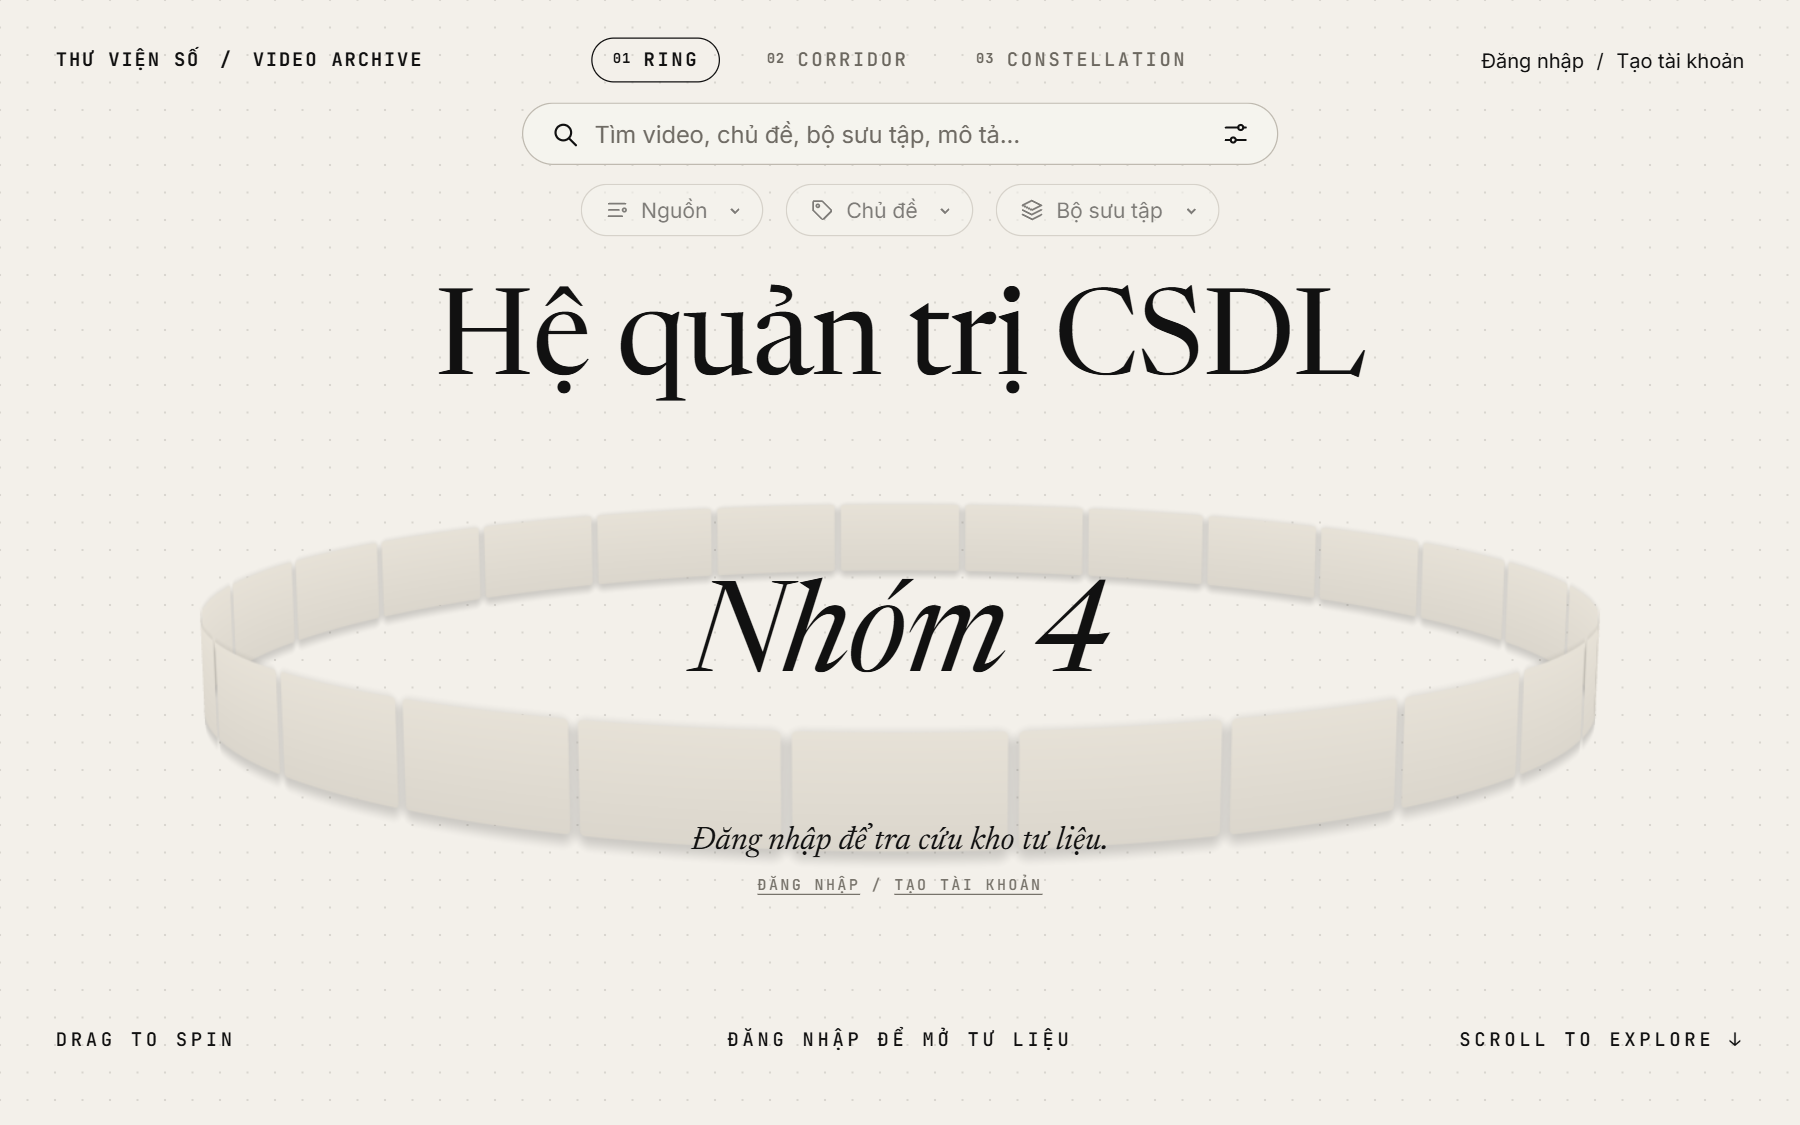
\includegraphics[width=0.9\textwidth]{orbit_landing.png}
\caption{Trang mở đầu công khai: khách chỉ thấy vòng trống, phải đăng nhập mới tra cứu được}
\label{fig:orbit_landing}
\end{figure}

\begin{figure}[H]
\centering
\begin{subfigure}{\textwidth}
\centering
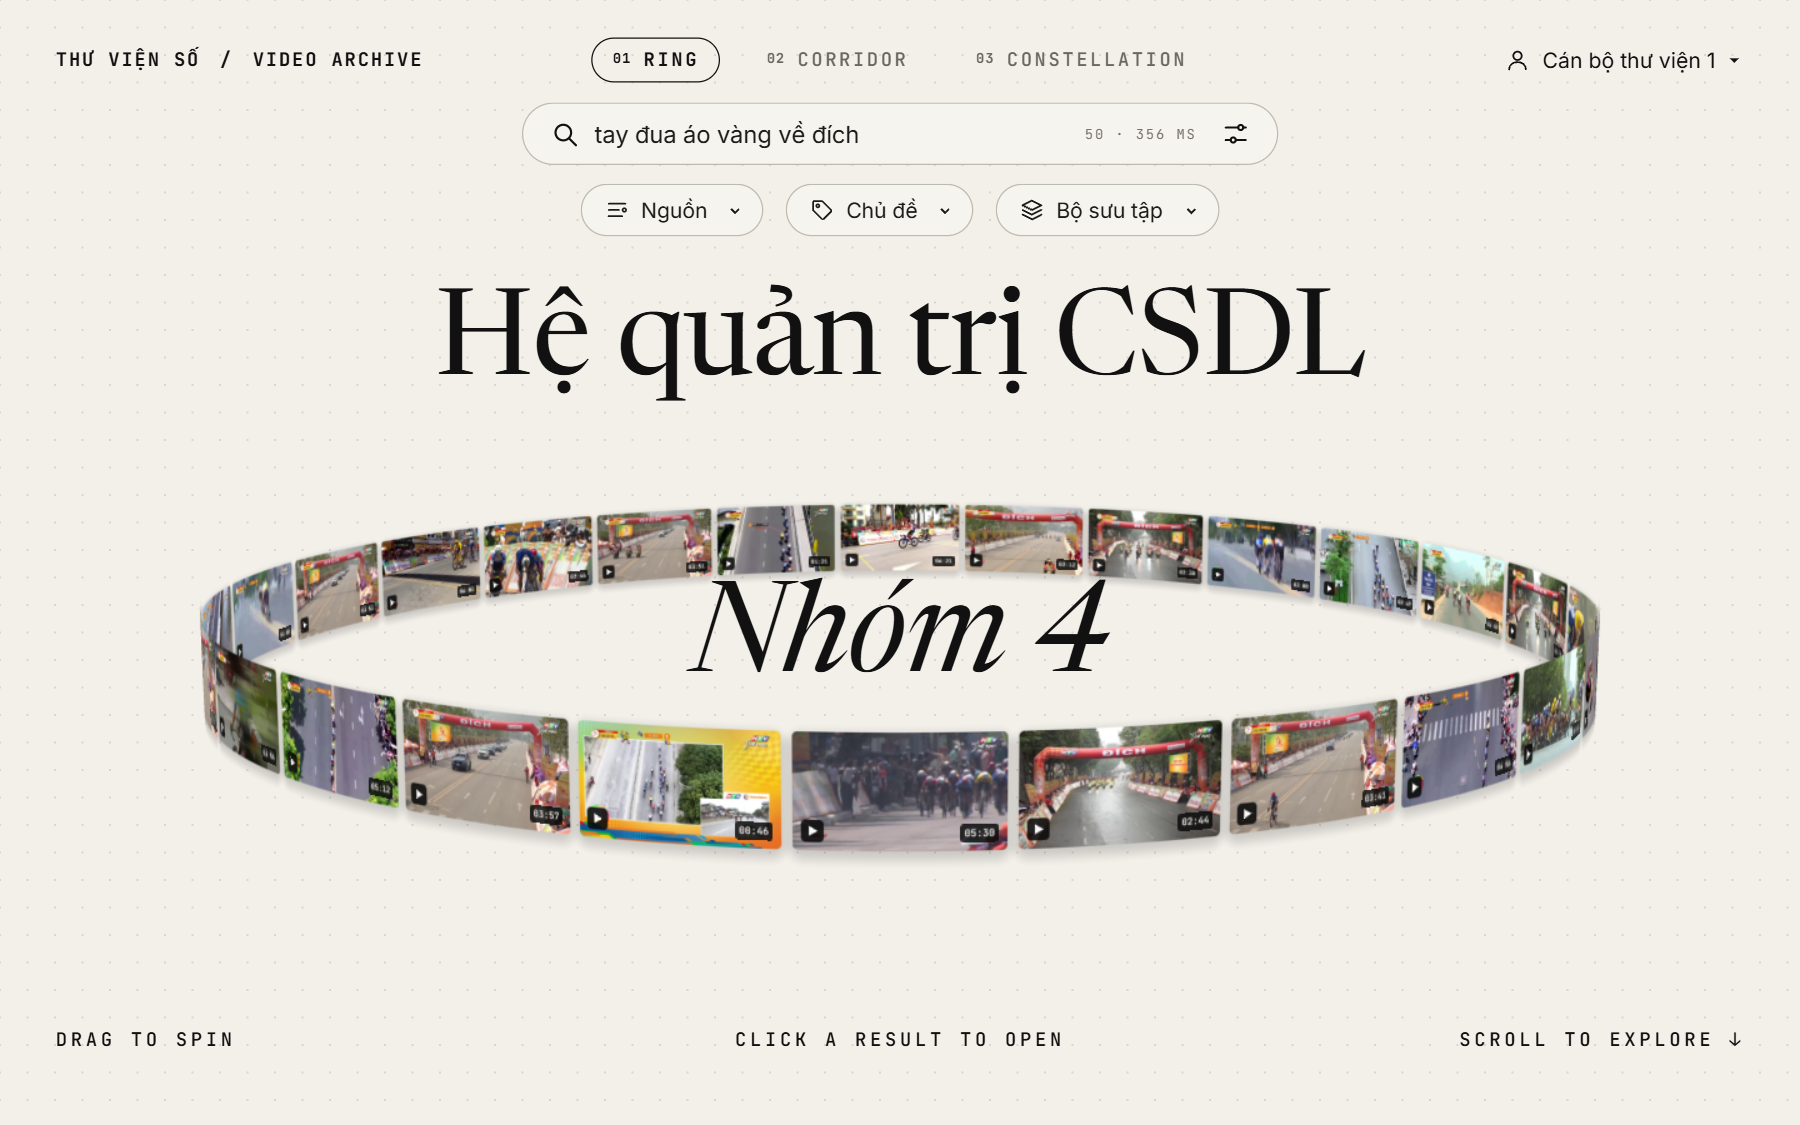
\includegraphics[width=0.82\textwidth]{orbit_ring.png}
\caption{Ring}
\end{subfigure}

\vspace{0.4em}
\begin{subfigure}{0.49\textwidth}
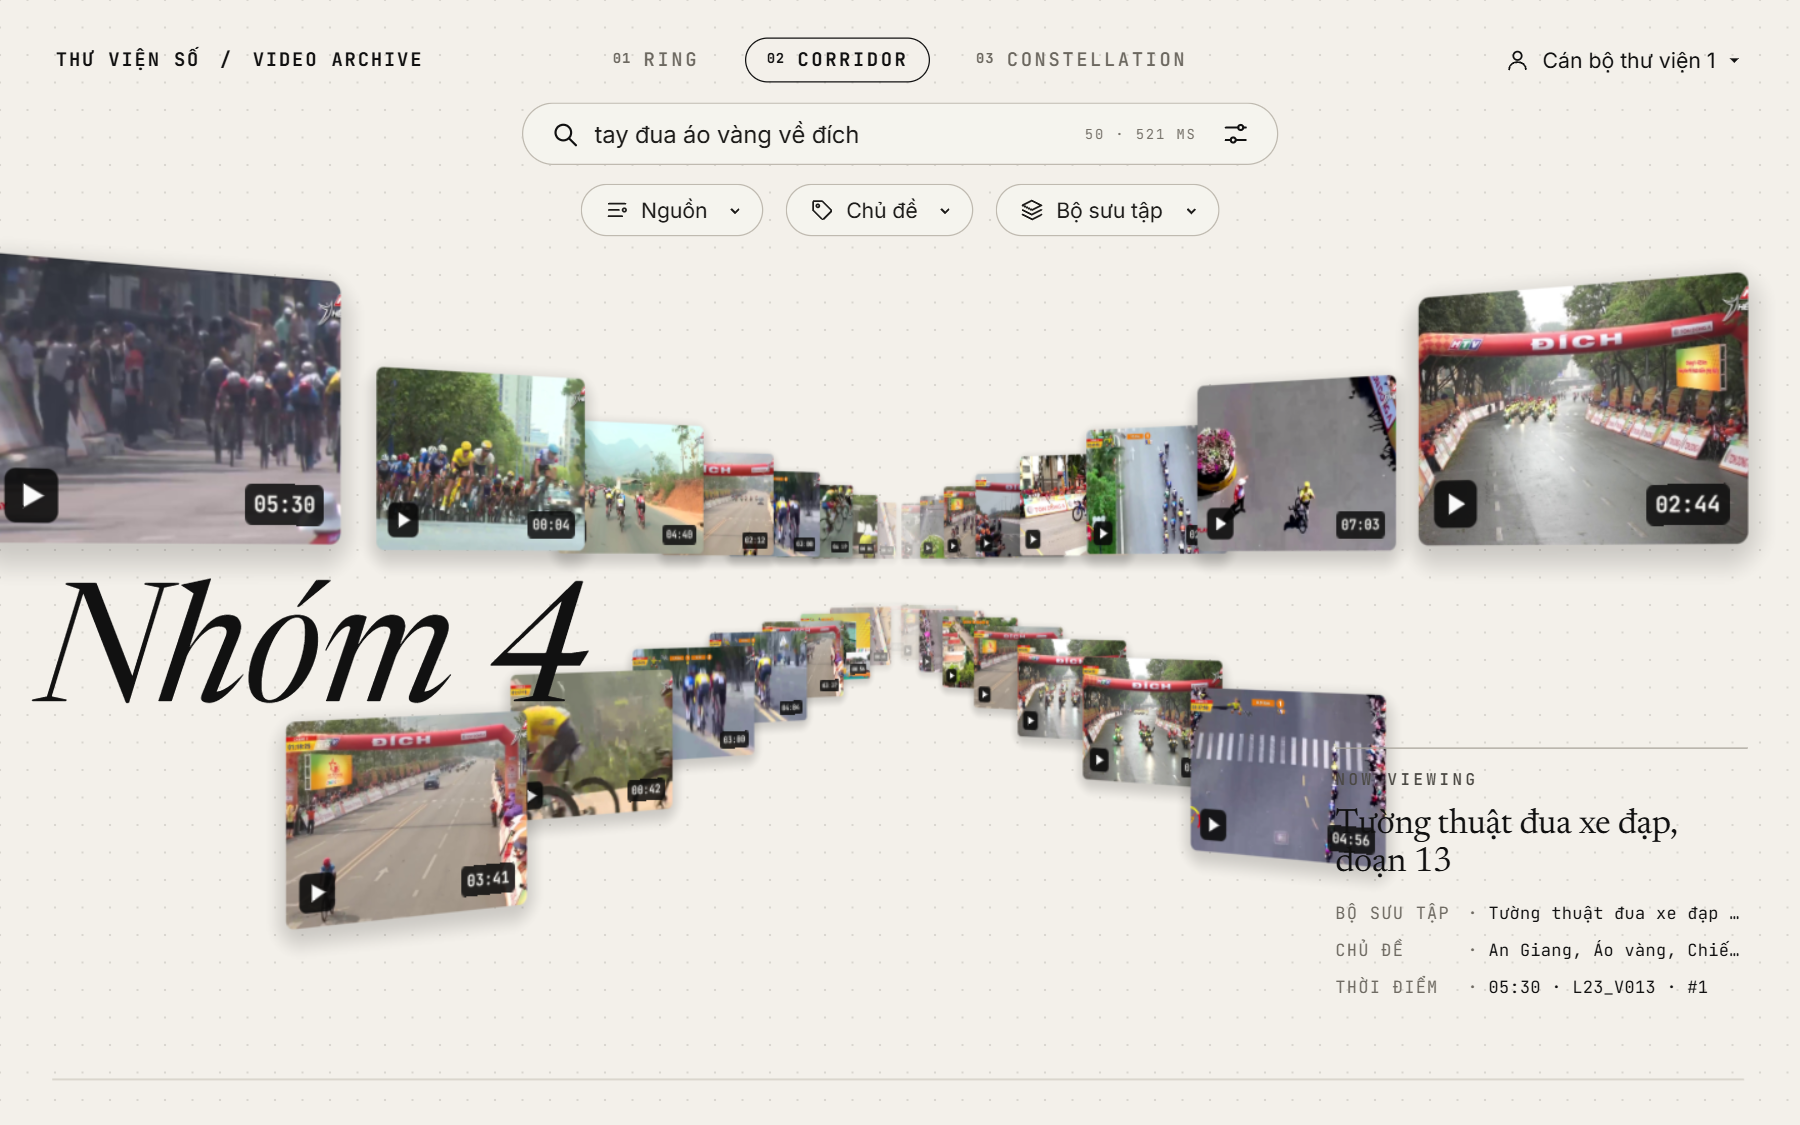
\includegraphics[width=\textwidth]{orbit_corridor.png}
\caption{Corridor}
\end{subfigure}
\hfill
\begin{subfigure}{0.49\textwidth}
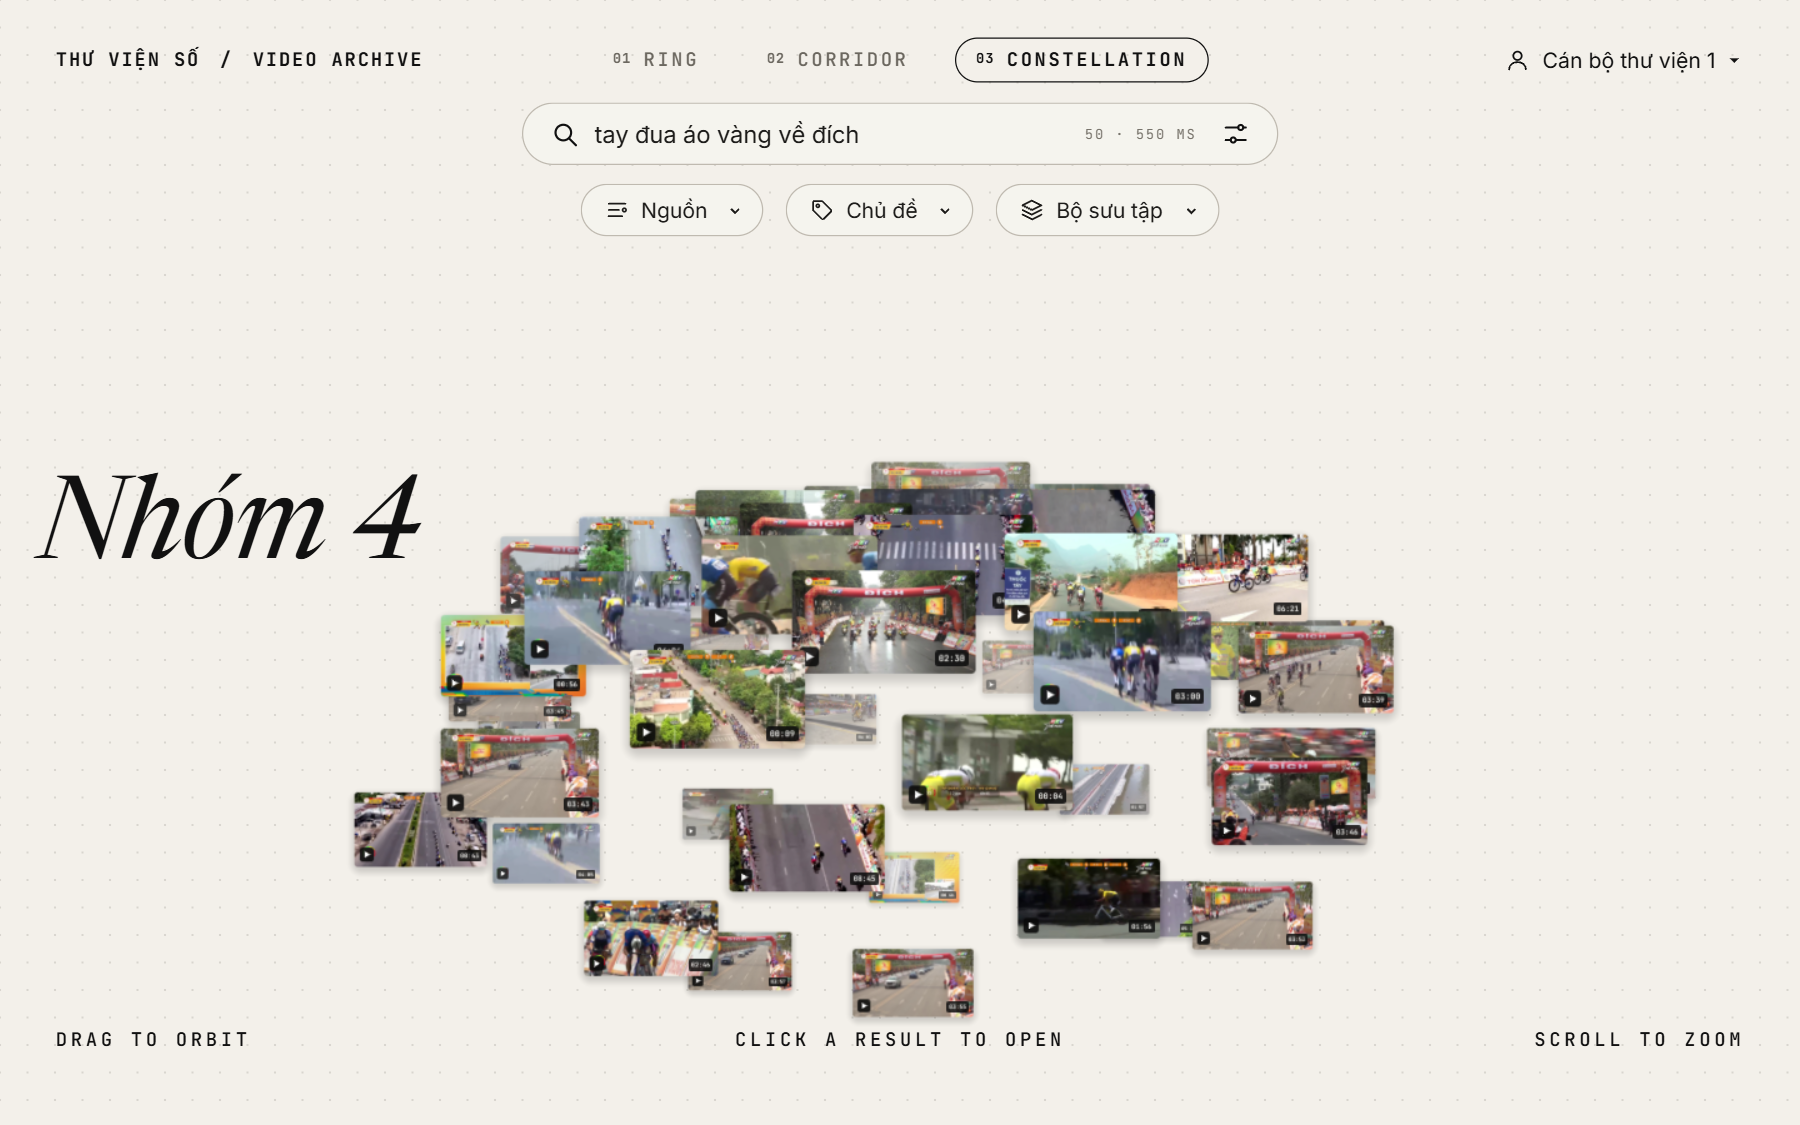
\includegraphics[width=\textwidth]{orbit_constellation.png}
\caption{Constellation}
\end{subfigure}
\caption{Ba chế độ hiển thị cùng một truy vấn ``tay đua áo vàng về đích'' (50 kết quả)}
\label{fig:orbit_views}
\end{figure}

\subsection{Tra cứu dạng danh sách và chi tiết khung hình}

Trang \texttt{/list} giữ dạng lưới truyền thống, thuận tiện khi cần đọc cột bằng chứng của
từng kết quả. Hình~\ref{fig:app_search} là kết quả cán bộ thư viện nhận được cho yêu cầu mẫu
YC-047 (``Người áo trắng chỉ phải cạnh biển HỒNG THÁI PHÚC LỘC''). Khung hình đúng
(L23\_V004, giây 171,8) đứng đầu nhờ chữ OCR (hạng 2 trong nguồn OCR), còn kênh hình ảnh xếp
nó hạng 30. Cả lượt tìm mất 291 ms. Dưới mỗi ảnh là cột \texttt{evidence} do thủ tục trả về.

\begin{figure}[H]
\centering
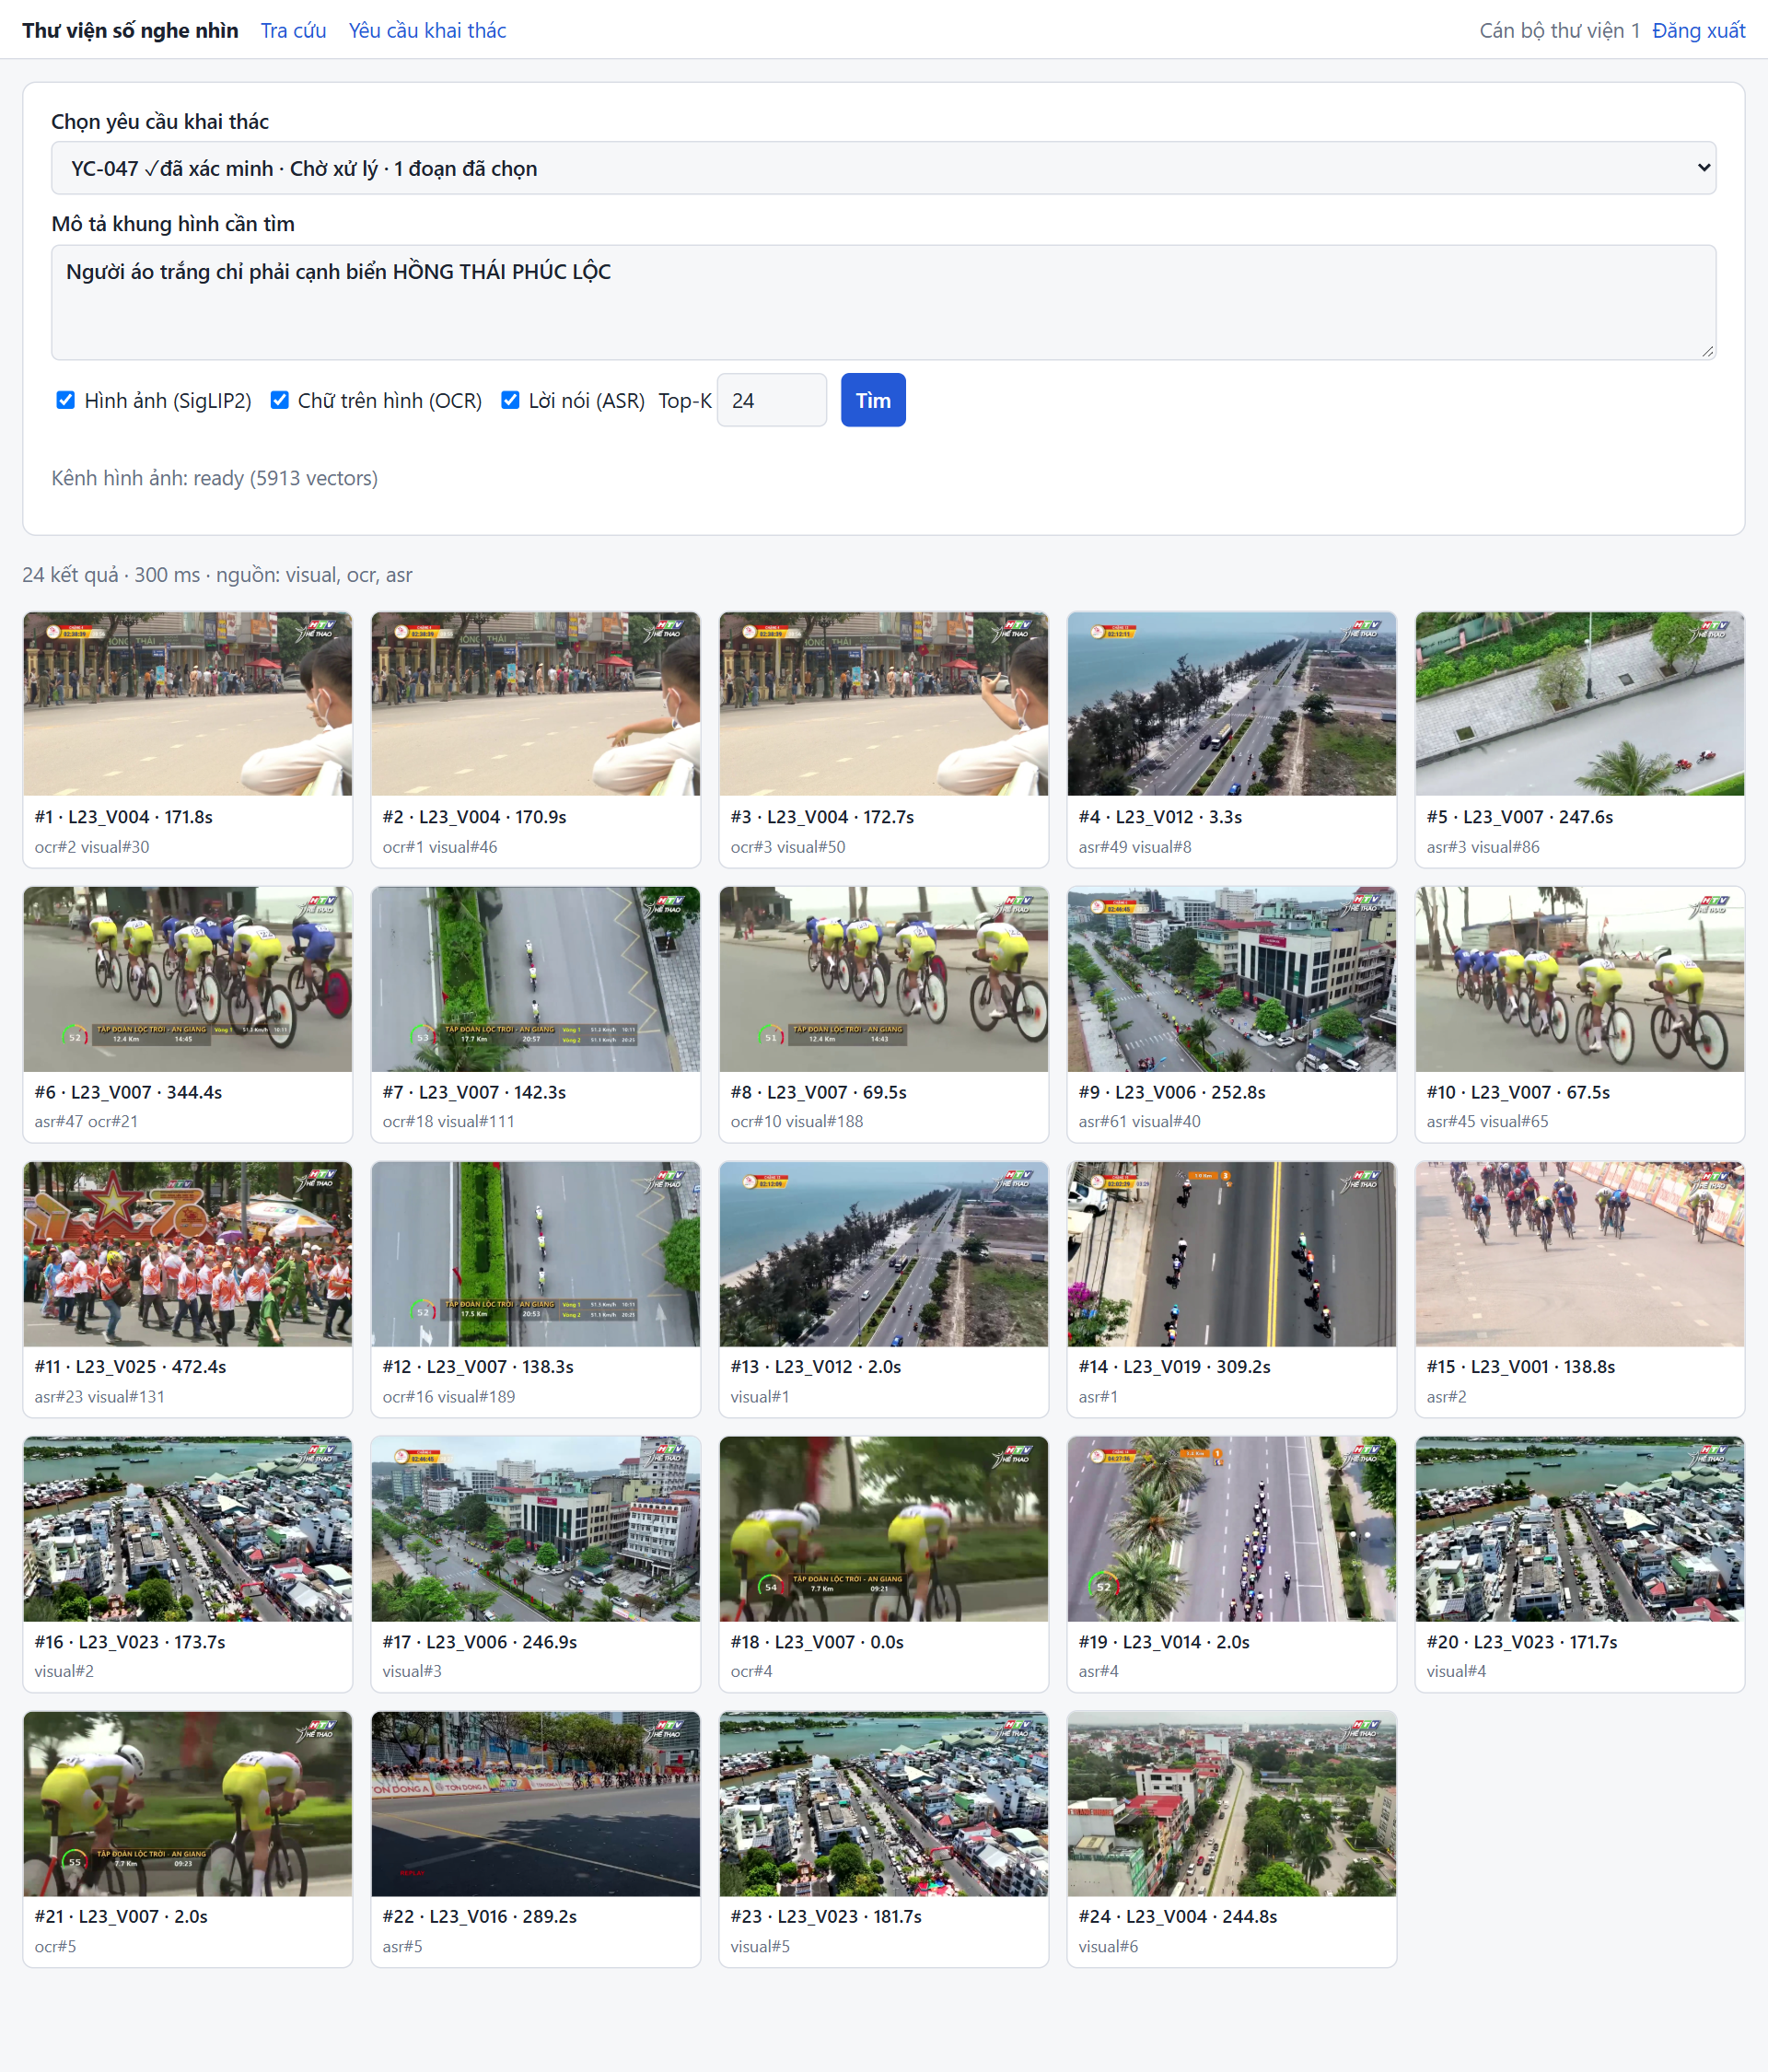
\includegraphics[width=0.9\textwidth]{app_search.png}
\caption{Trang tra cứu dạng danh sách: yêu cầu YC-047 gộp cả ba nguồn, khung hình đúng xếp hạng 1}
\label{fig:app_search}
\end{figure}

\begin{figure}[H]
\centering
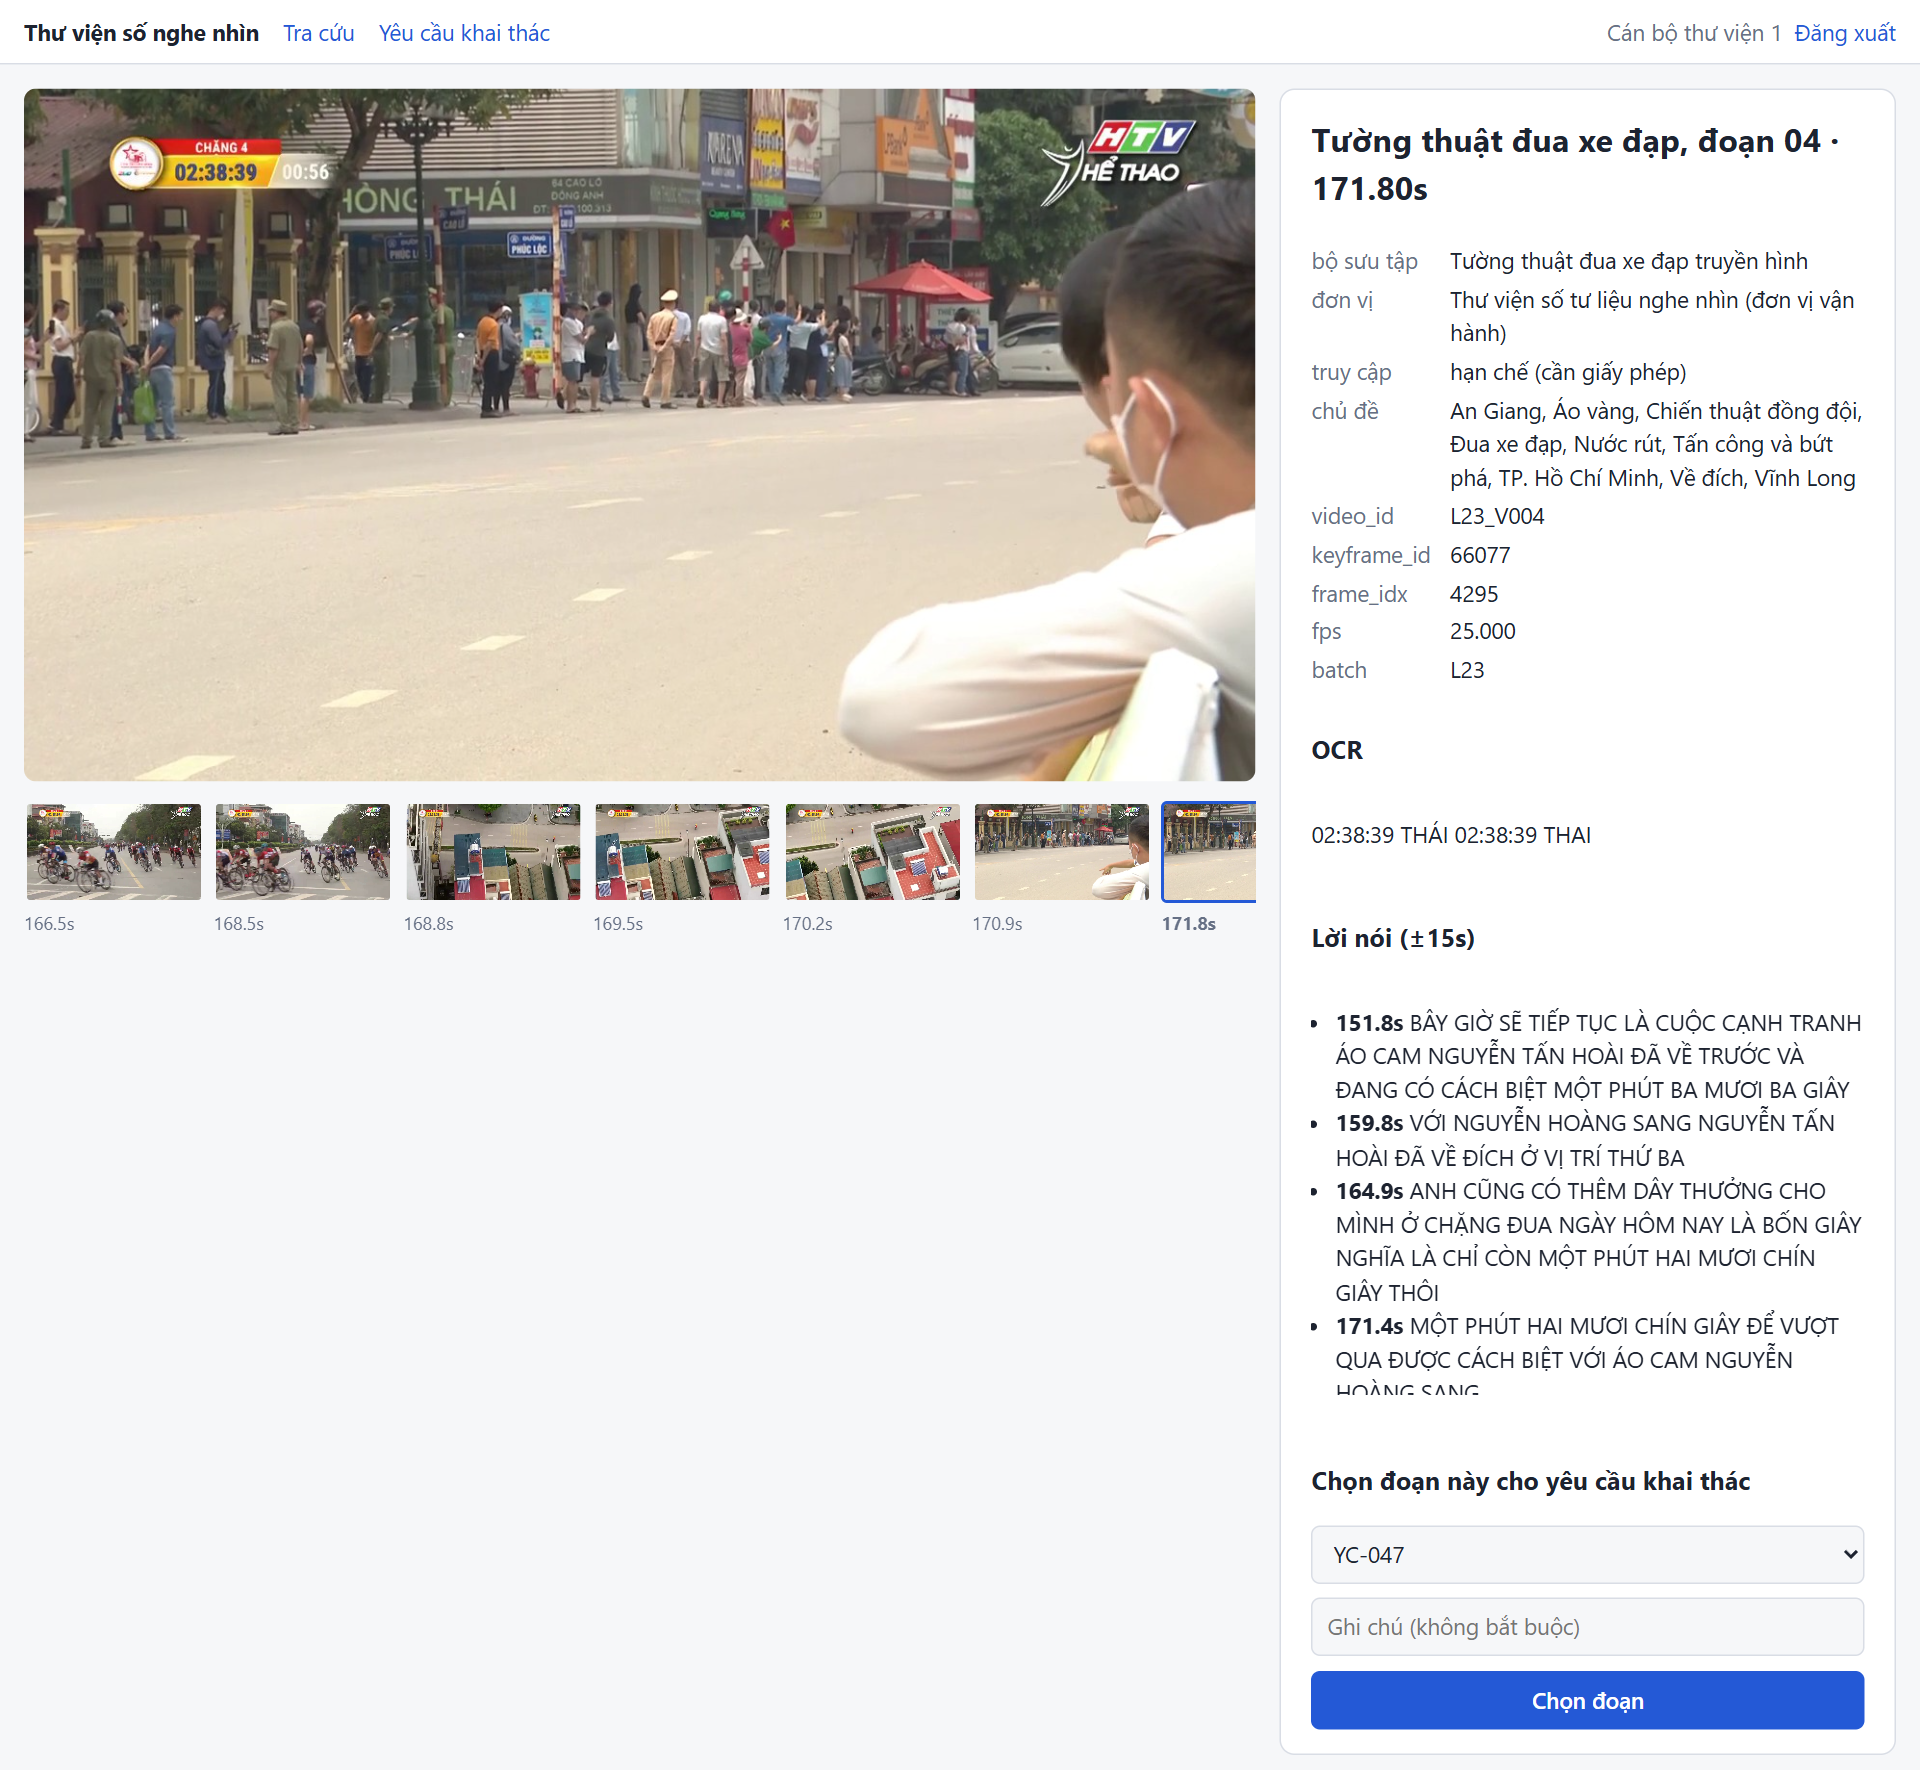
\includegraphics[width=0.9\textwidth]{app_frame.png}
\caption{Trang chi tiết khung hình: phiếu mô tả video (bộ sưu tập, đơn vị, mức truy cập, chủ đề), khung lân cận, chữ OCR, lời nói $\pm$15 giây}
\label{fig:app_frame}
\end{figure}

\subsection{Yêu cầu khai thác}

Trang ``Yêu cầu khai thác'' đọc từ \texttt{v\_request\_progress}. Cán bộ thư viện thấy mọi yêu
cầu, lọc được theo trạng thái, và có nút cấp phép (chọn thời hạn) hoặc từ chối cho yêu cầu
đang chờ; nút cấp phép chỉ hiện khi yêu cầu đã có đoạn tư liệu (Hình~\ref{fig:app_requests}).
Bạn đọc chỉ thấy yêu cầu của mình, có biểu mẫu gửi yêu cầu mới, và tệp CSV xuất ra cũng chỉ
gồm đoạn tư liệu của các yêu cầu đó (Hình~\ref{fig:app_requests_reader}). Nếu ai đó gửi thẳng
yêu cầu HTTP để cấp phép cho một yêu cầu chưa có đoạn nào, thủ tục báo lỗi 50006 và trang
hiển thị thông báo tương ứng.

\begin{figure}[H]
\centering
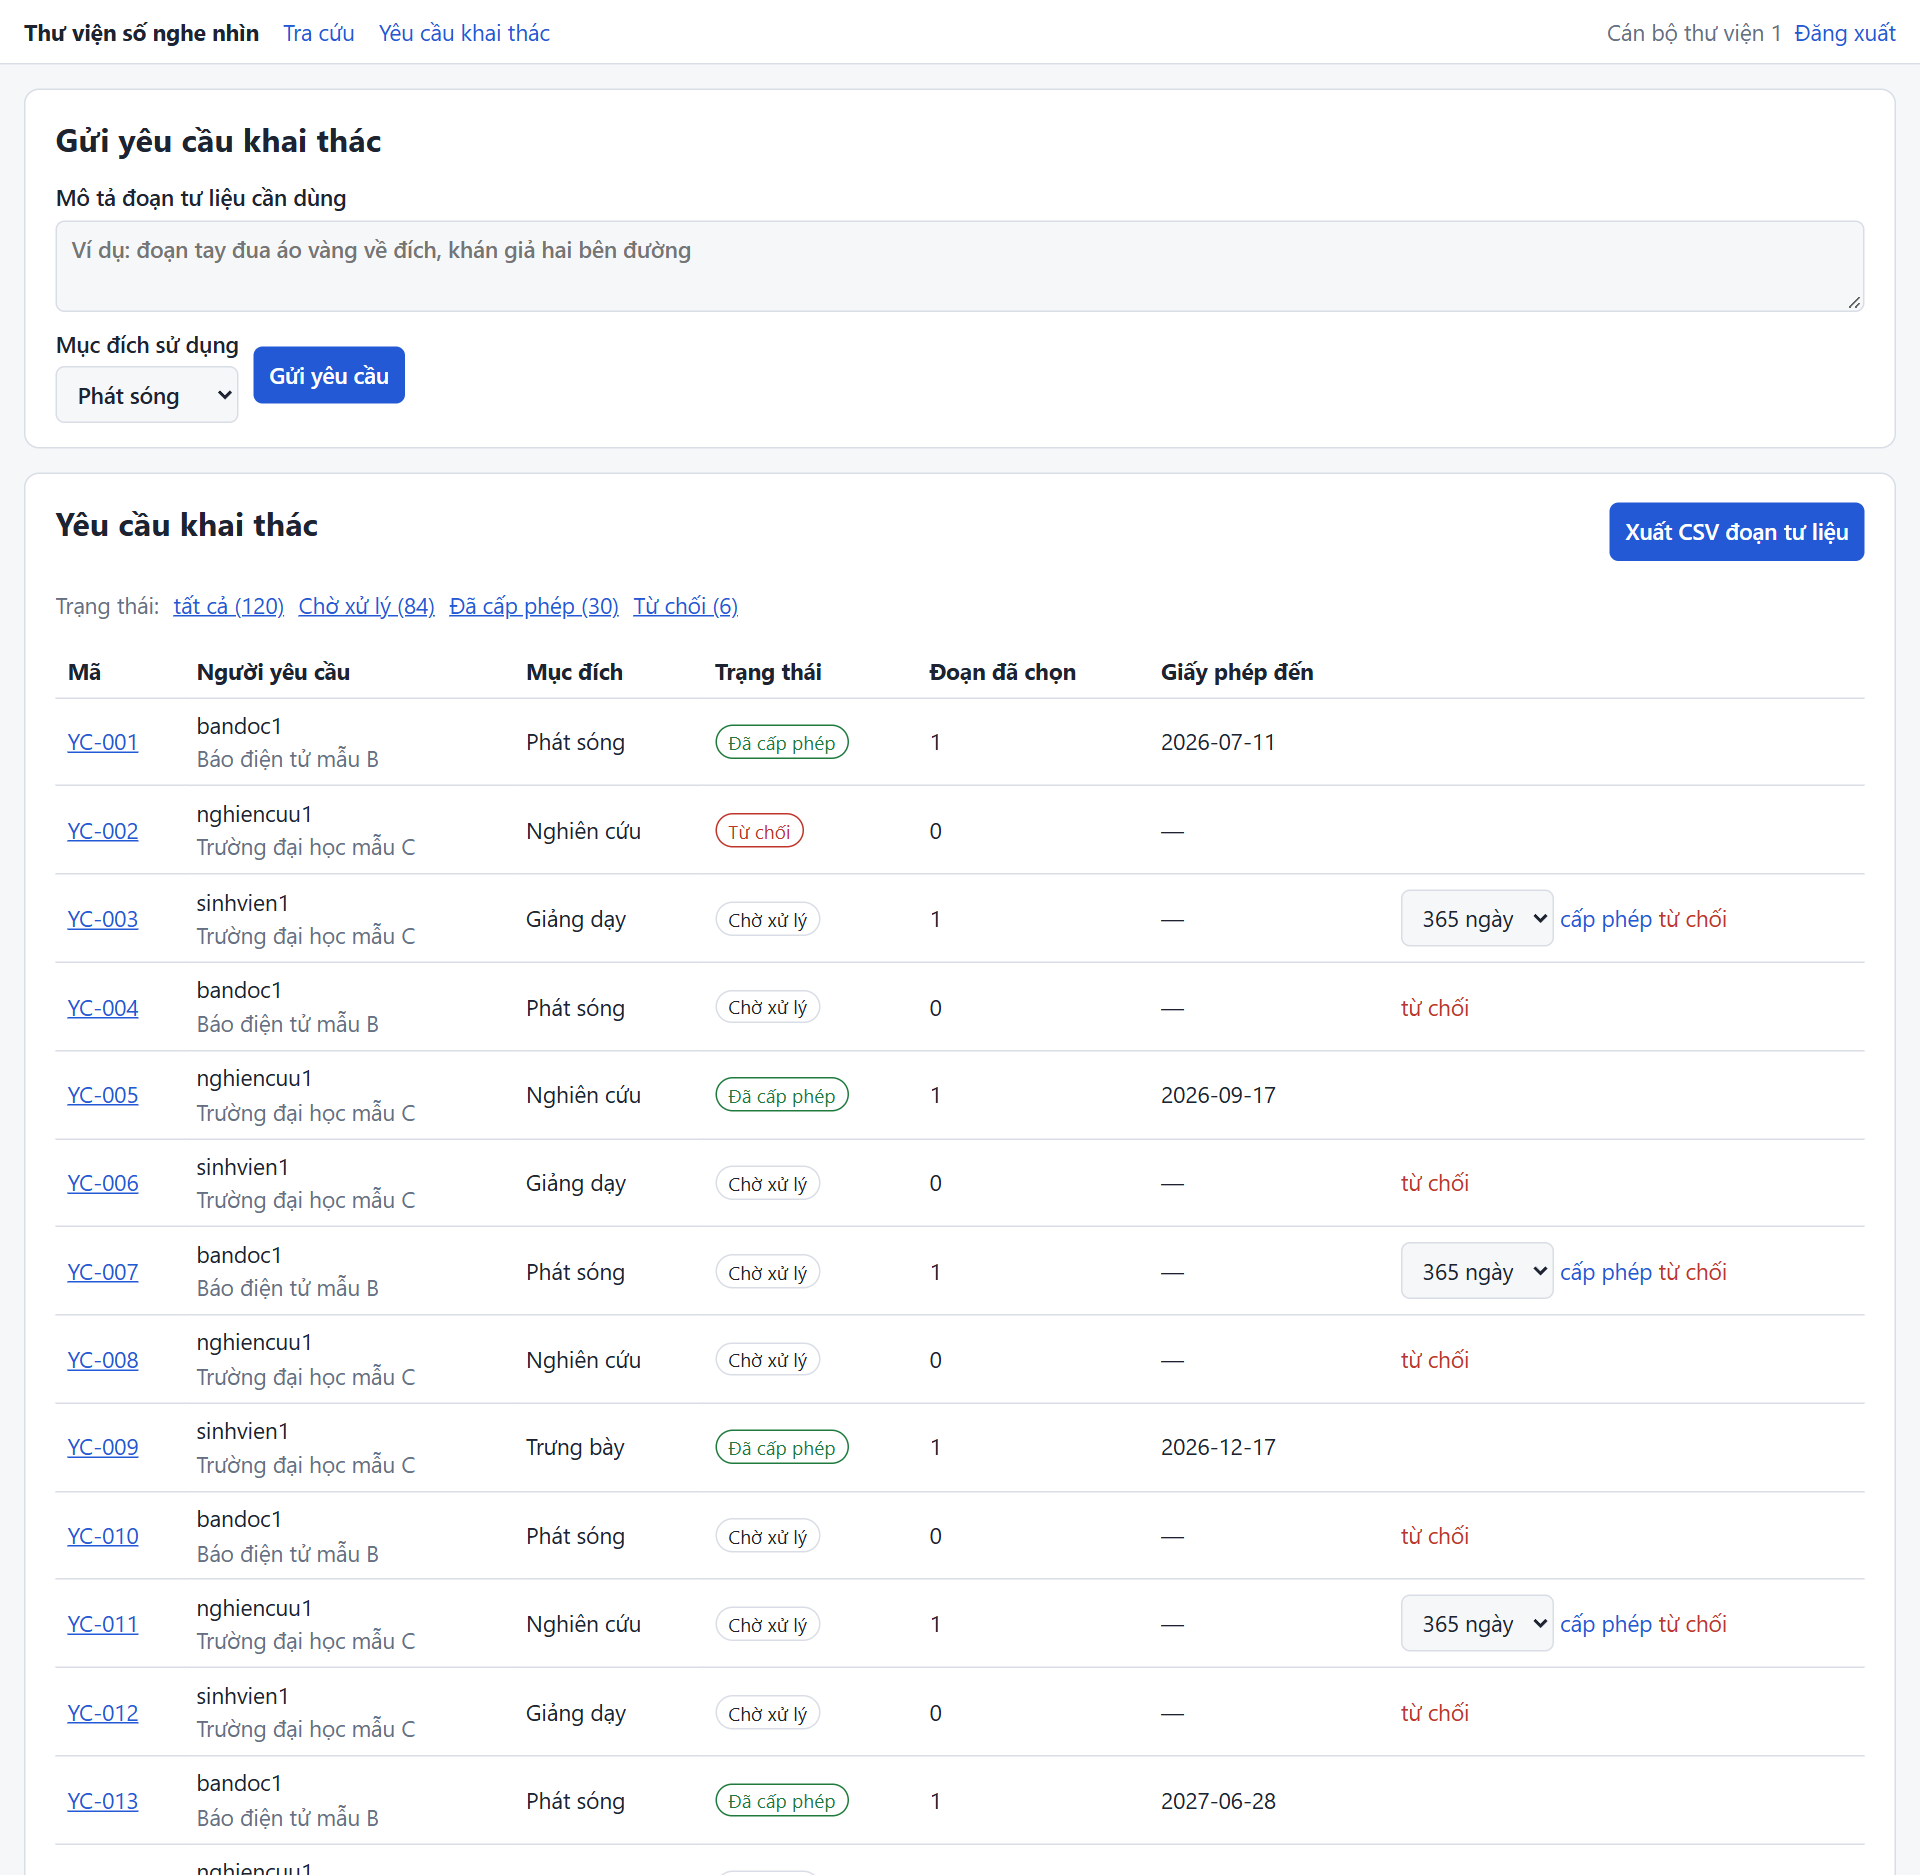
\includegraphics[width=0.9\textwidth]{app_requests.png}
\caption{Trang yêu cầu khai thác của cán bộ thư viện: trạng thái, hạn giấy phép, cấp phép hoặc từ chối}
\label{fig:app_requests}
\end{figure}

\begin{figure}[H]
\centering
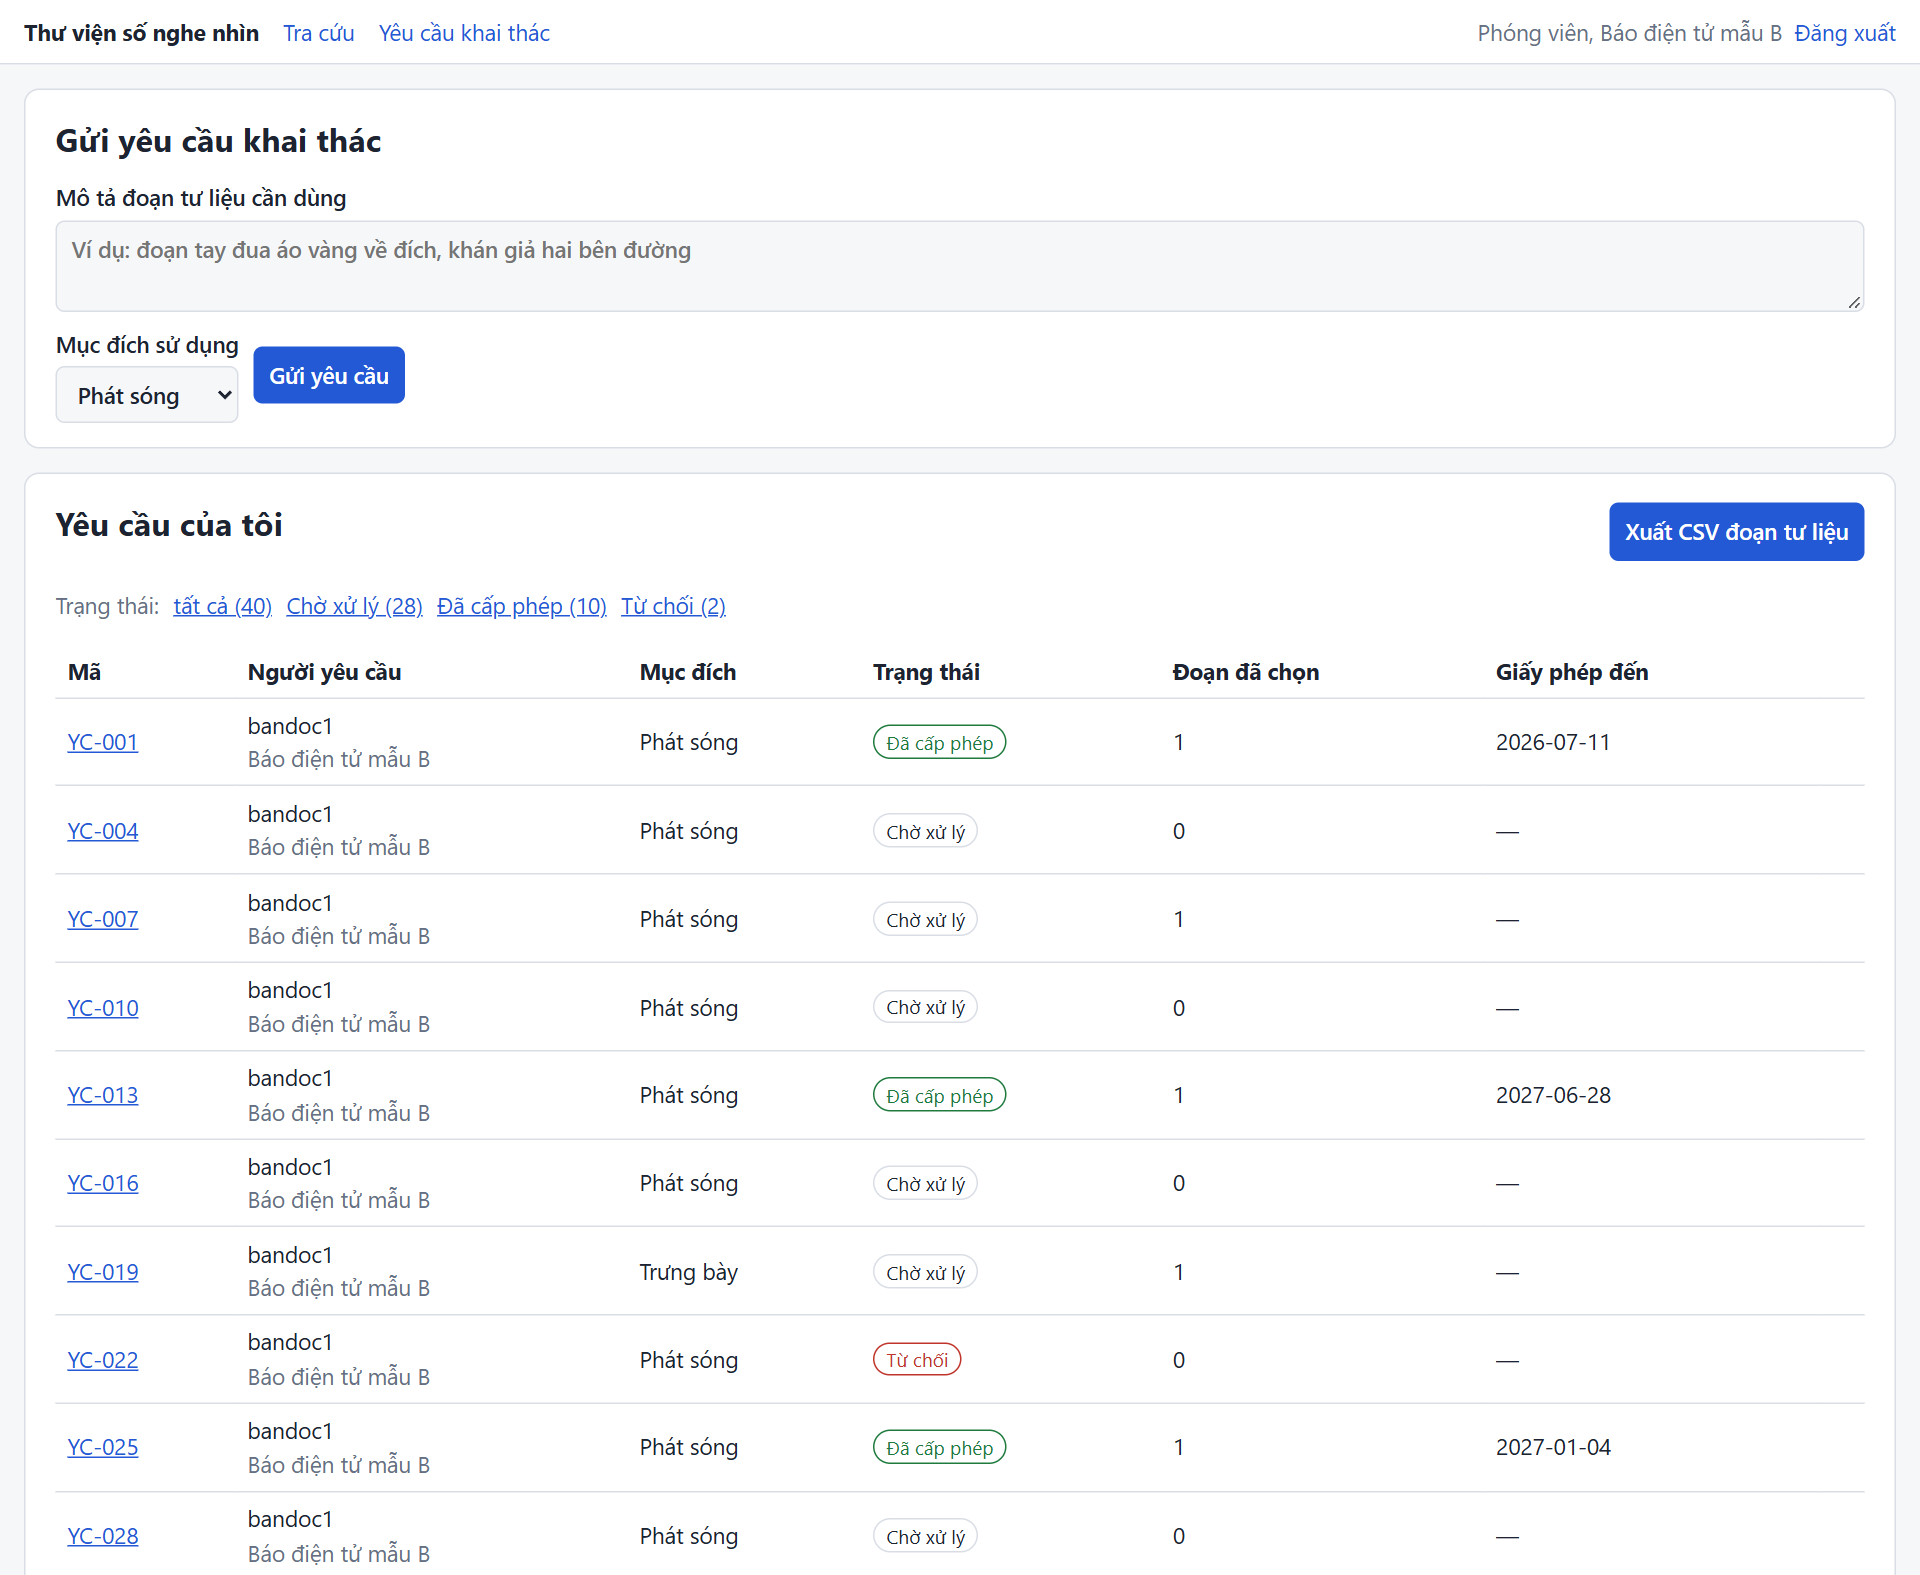
\includegraphics[width=0.9\textwidth]{app_requests_reader.png}
\caption{Cùng trang đó với bạn đọc \texttt{bandoc1}: gửi yêu cầu mới, chỉ thấy 40 yêu cầu của mình}
\label{fig:app_requests_reader}
\end{figure}

\subsection{Tự đăng ký tài khoản bạn đọc}
\label{sec:register}

Khách có thể tự tạo tài khoản bạn đọc ở trang \texttt{/register}
(Hình~\ref{fig:orbit_register}); biến cấu hình \texttt{ARCHIVE\_SELF\_REGISTRATION=0} tắt
trang này và khi đó chỉ quản trị viên tạo được tài khoản. Vì người đăng ký chưa có phiên làm
việc, không thể dựa vào \texttt{SESSION\_CONTEXT} để kiểm tra quyền như các thủ tục ở trên.
Thủ tục \texttt{sp\_register\_reader} vì thế tự khoá cứng những gì được phép:
\begin{itemize}
    \item luôn gán đúng vai trò \texttt{reader}, không nhận tham số vai trò, không gắn đơn vị;
    đối tượng ngoài danh sách (kể cả \texttt{staff}) bị đổi thành \texttt{other};
    \item từ chối mật khẩu chưa băm (giá trị không bắt đầu bằng \texttt{scrypt\$}) với lỗi
    50007, nên dù tầng web có lỗi cũng không lưu được mật khẩu dạng rõ;
    \item thêm người dùng, vai trò và dòng nhật ký \texttt{user.register} trong \textit{một}
    giao dịch.
\end{itemize}
\texttt{archive\_app} chỉ được \texttt{EXECUTE} thủ tục này, không có quyền \texttt{INSERT} trên
\texttt{users}. Ở tầng web, biểu mẫu có mã chống giả mạo yêu cầu (CSRF), mỗi thiết bị tạo tối
đa 5 tài khoản mỗi giờ, và đăng nhập sai 10 lần trong 5 phút thì bị tạm khoá. CSDL đã tạo
trước khi có tính năng này cần chạy thêm \texttt{db/migrations/001\_self\_registration.sql}.

\begin{lstlisting}[caption={Phần lõi của sp\_register\_reader}, label={lst:register}]
IF @user_type IS NULL OR @user_type NOT IN ('journalist', 'researcher', 'student', 'other')
    SET @user_type = 'other';
IF @password_hash IS NULL OR @password_hash NOT LIKE 'scrypt$%'
    THROW 50007, N'Password must be hashed with scrypt', 1;
BEGIN TRY
    BEGIN TRANSACTION;
        INSERT INTO dbo.users (username, full_name, password_hash, organization_id, user_type)
        VALUES (LOWER(LTRIM(RTRIM(@username))), COALESCE(LTRIM(RTRIM(@full_name)), N''),
                @password_hash, NULL, @user_type);
        DECLARE @user_id INT = SCOPE_IDENTITY();
        INSERT INTO dbo.user_roles (user_id, role_id)
        SELECT @user_id, role_id FROM dbo.roles WHERE role_name = 'reader';
        IF @@ROWCOUNT <> 1 THROW 50002, N'Role reader missing', 1;
        INSERT INTO dbo.audit_log (user_id, action, detail)
        VALUES (@user_id, 'user.register', LOWER(LTRIM(RTRIM(@username))));
    COMMIT TRANSACTION;
    SELECT @user_id AS user_id;
END TRY
BEGIN CATCH
    IF @@TRANCOUNT > 0 ROLLBACK TRANSACTION;
    THROW;
END CATCH;
\end{lstlisting}

\begin{figure}[H]
\centering
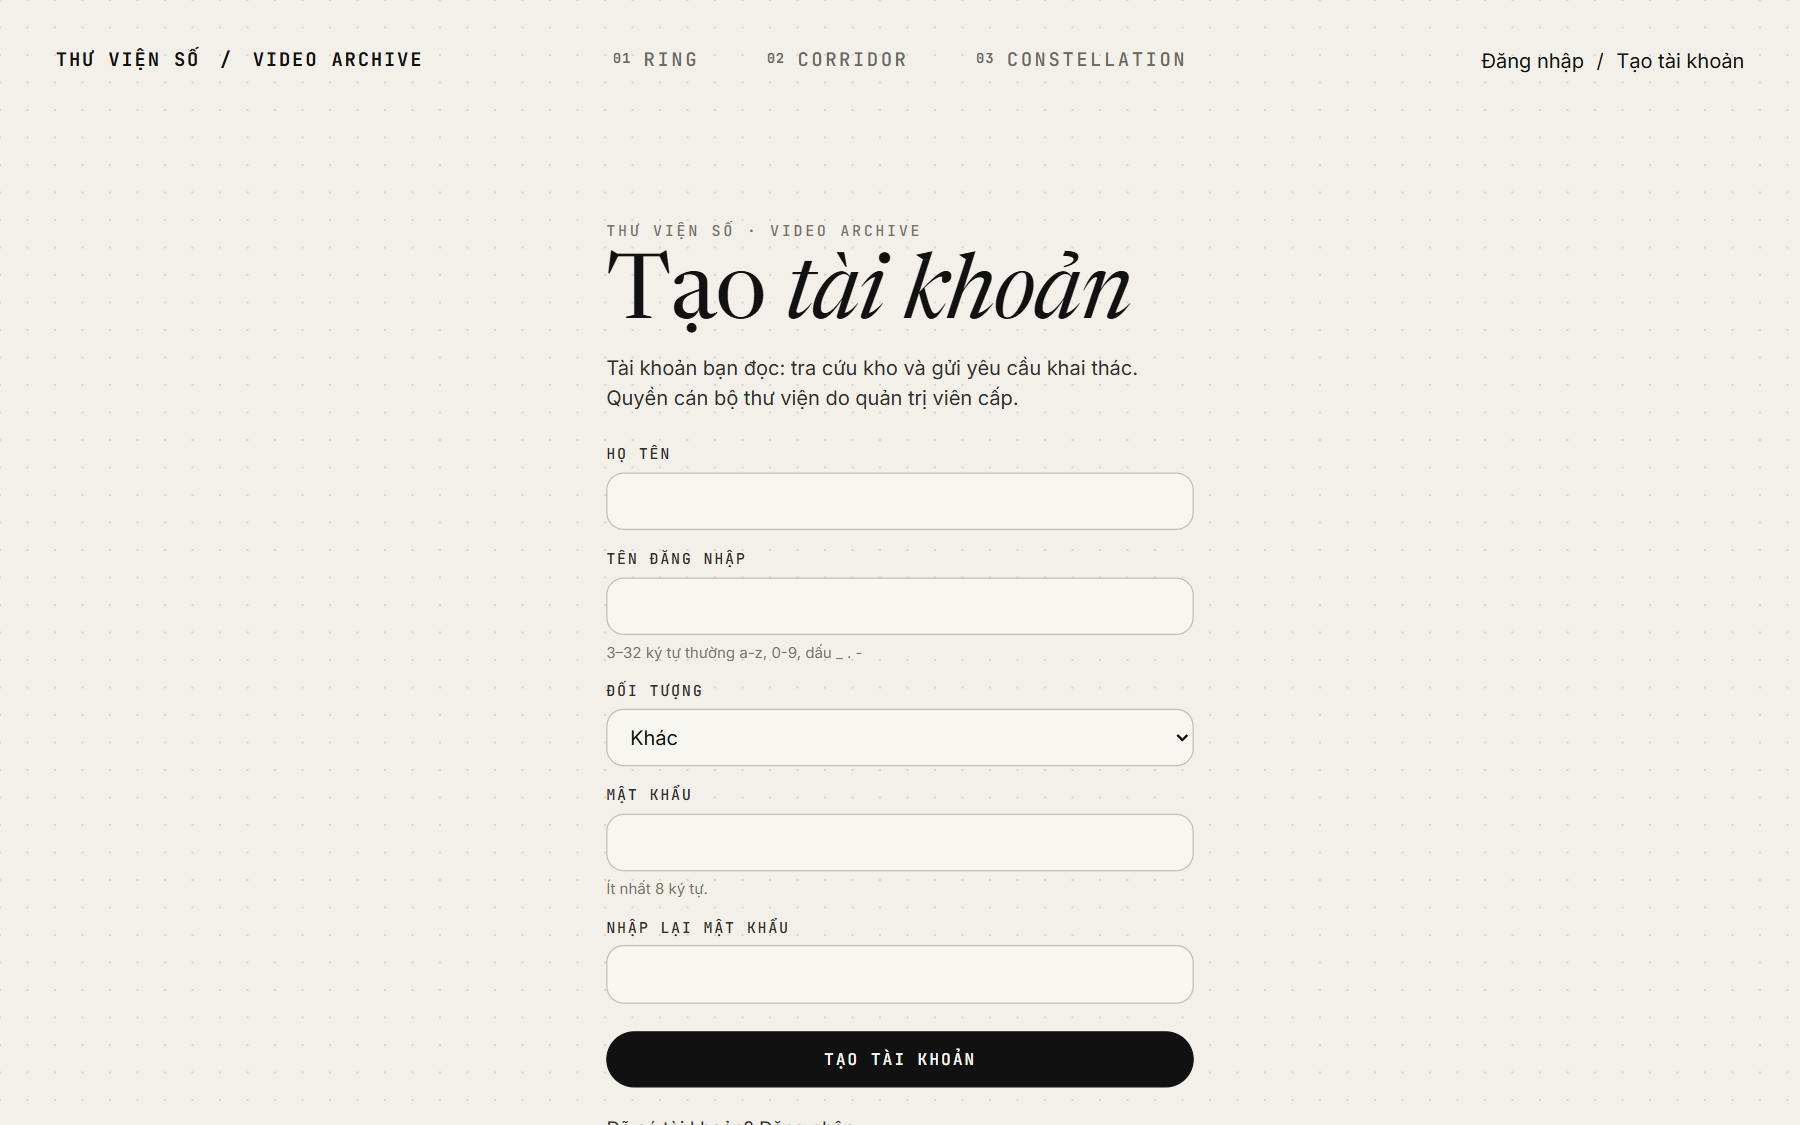
\includegraphics[width=0.75\textwidth]{orbit_register.png}
\caption{Trang tự đăng ký: chỉ tạo được tài khoản bạn đọc}
\label{fig:orbit_register}
\end{figure}

\subsection{Quản trị và đánh giá}

\begin{figure}[H]
\centering
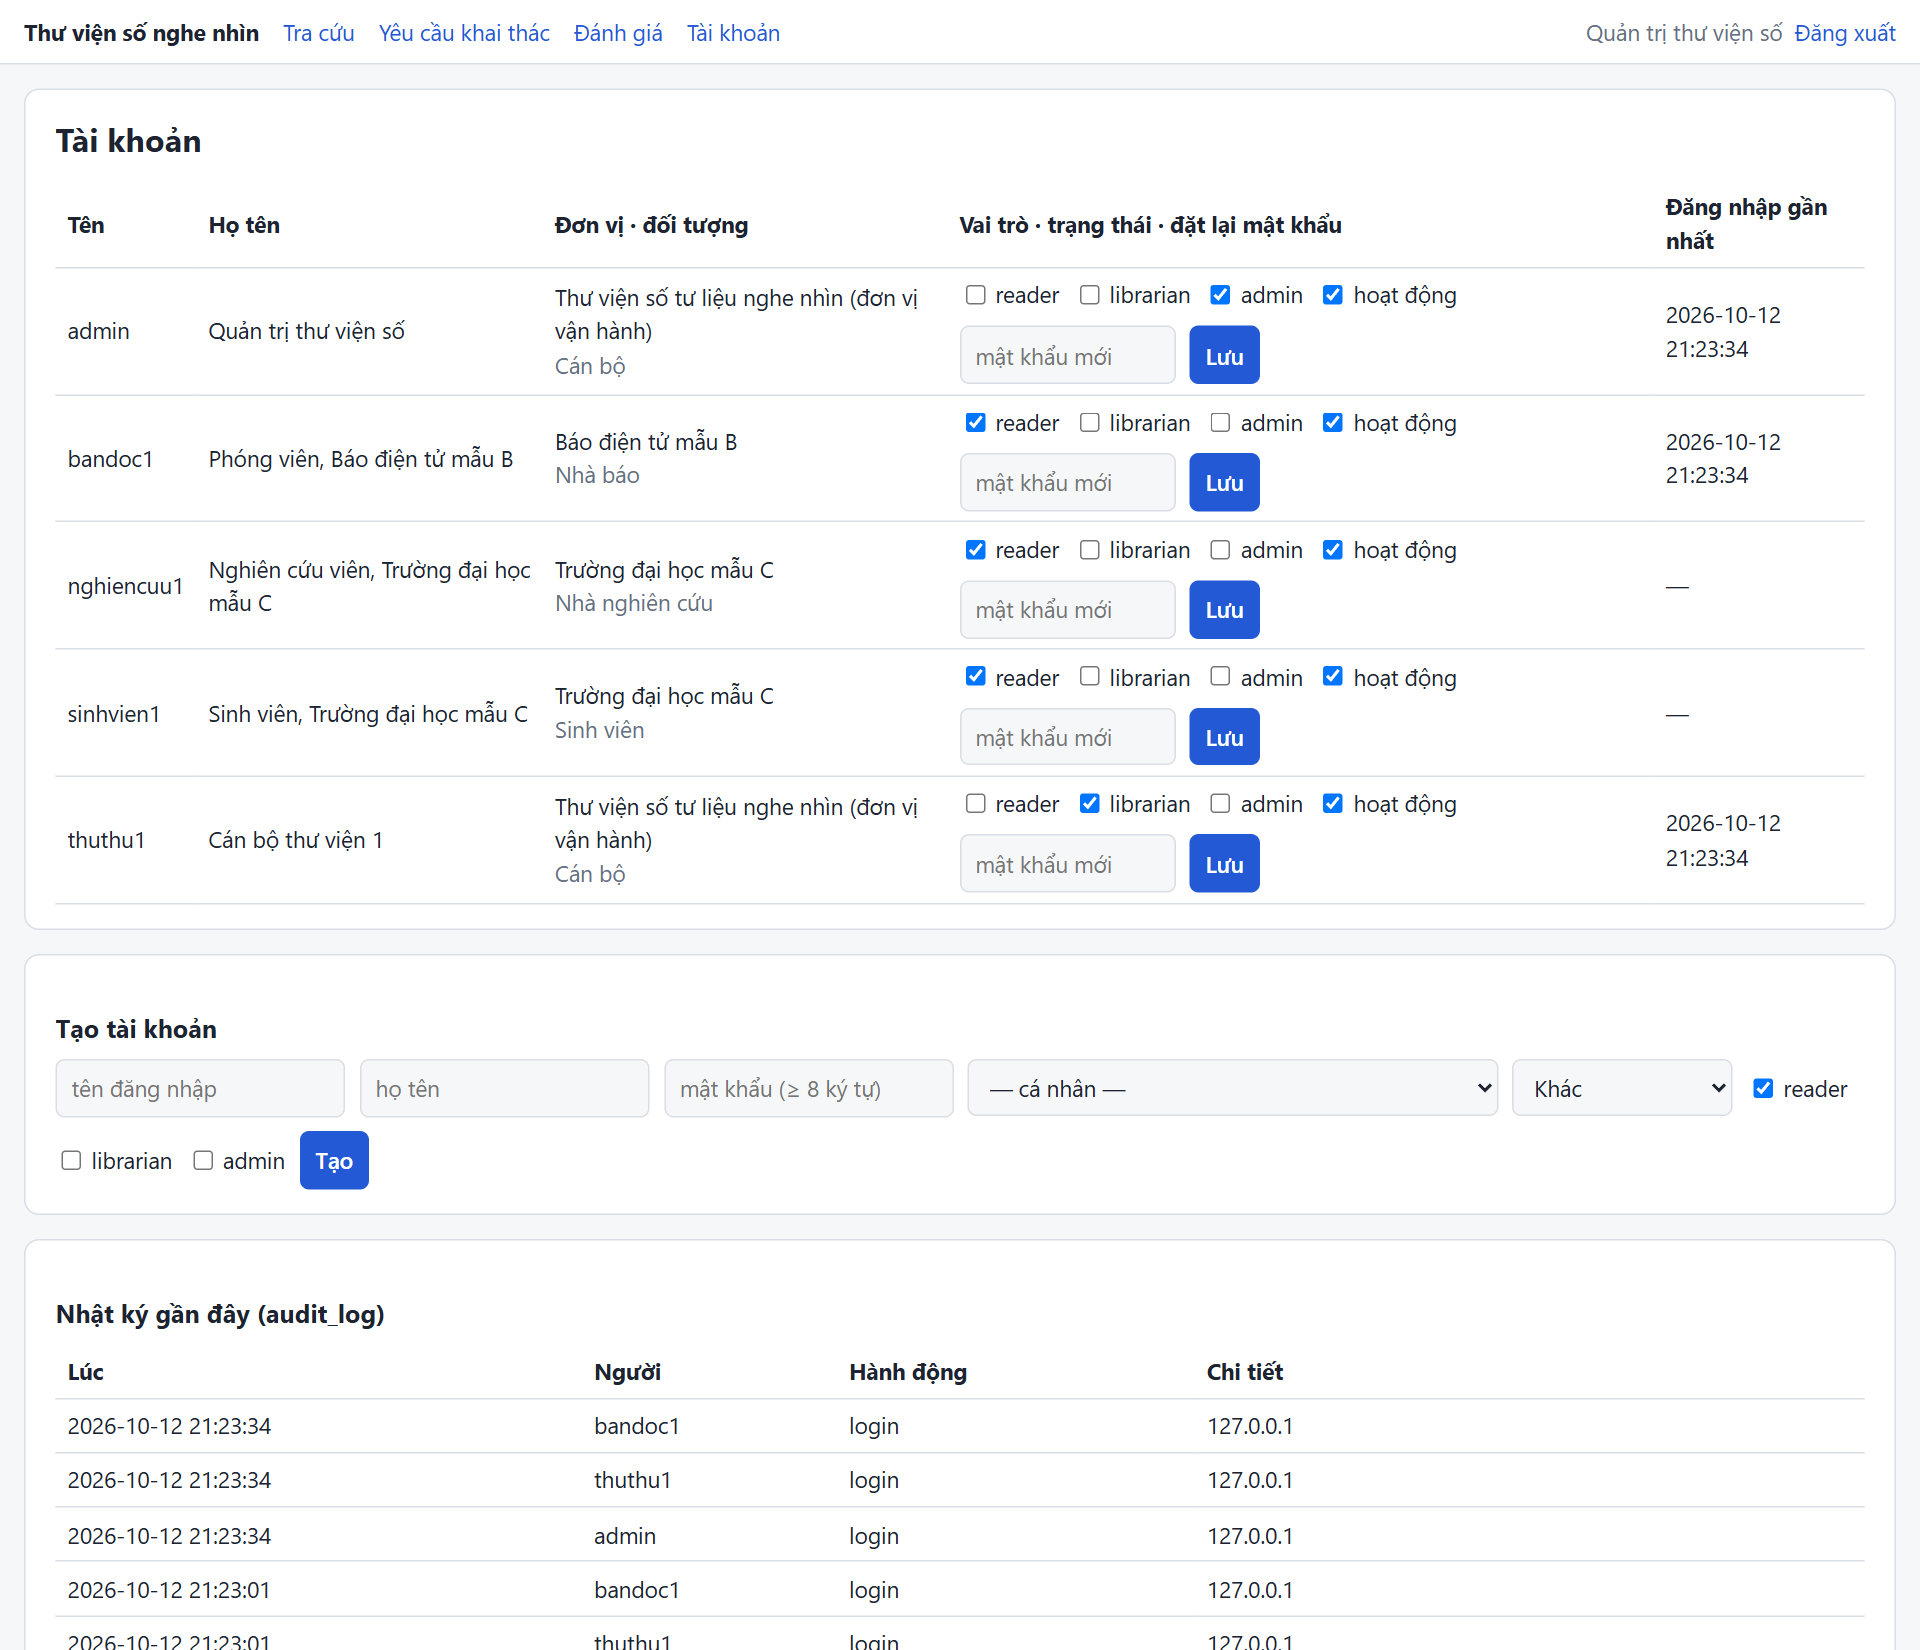
\includegraphics[width=0.9\textwidth]{app_users.png}
\caption{Trang quản trị tài khoản (đơn vị, đối tượng, vai trò) và nhật ký do trigger ghi}
\label{fig:app_users}
\end{figure}

\begin{figure}[H]
\centering
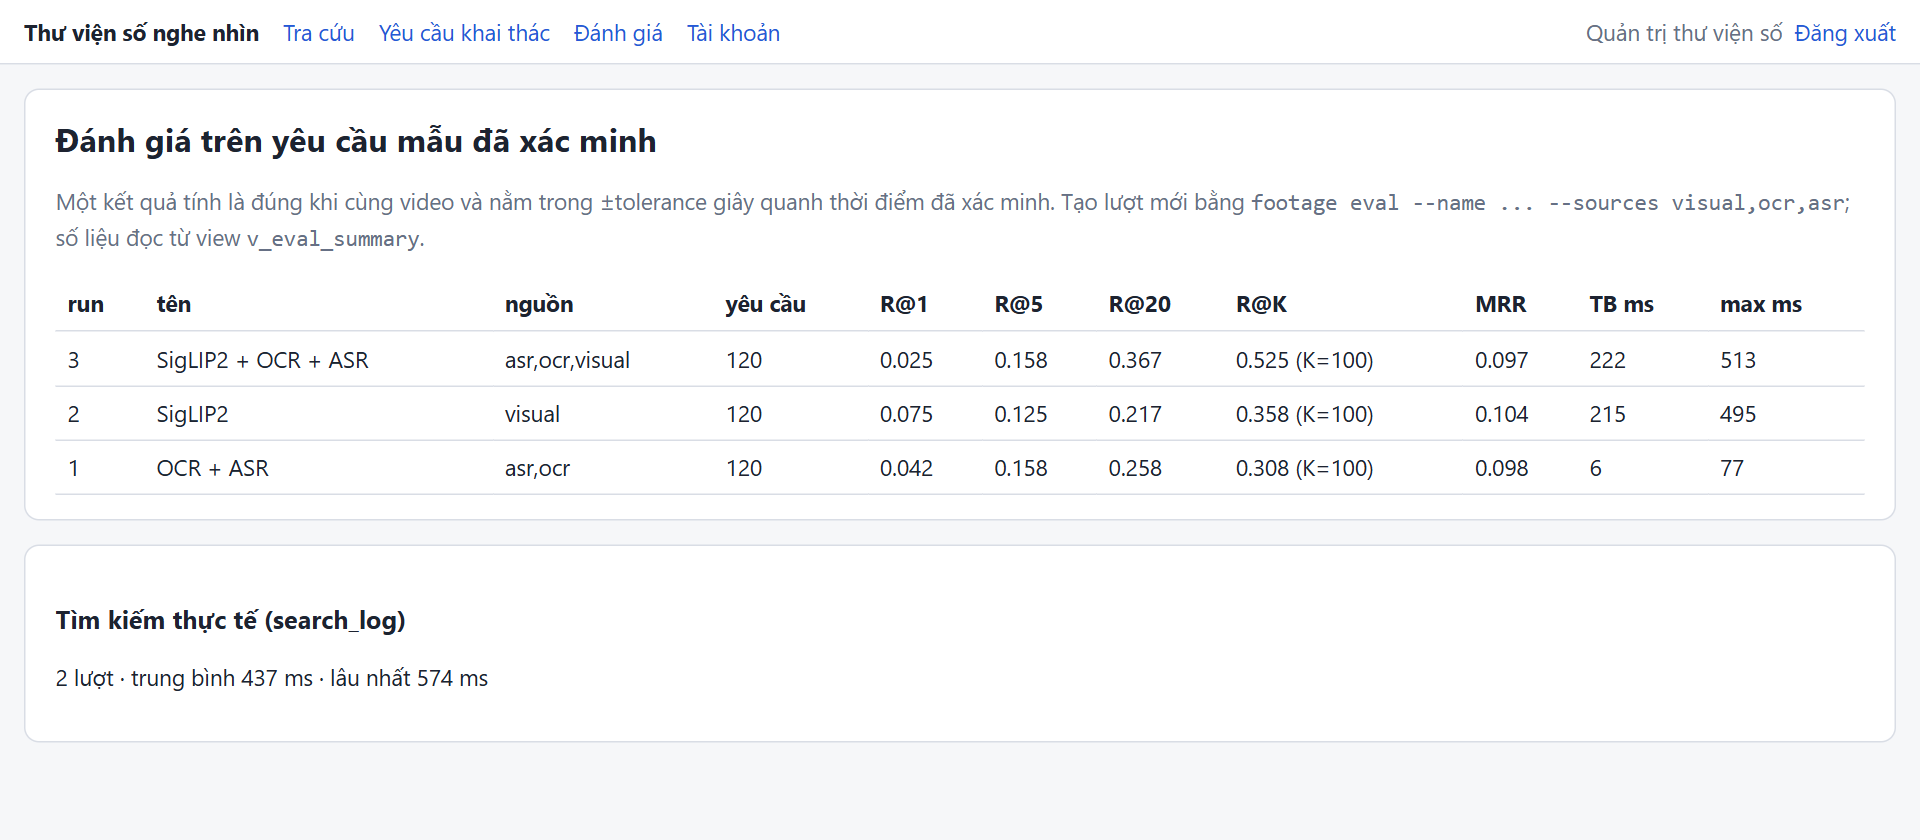
\includegraphics[width=0.9\textwidth]{app_eval.png}
\caption{Trang kết quả đánh giá, đọc từ \texttt{v\_eval\_summary}}
\label{fig:app_misc}
\end{figure}

\section{Đánh giá hiệu quả tìm kiếm}

\subsection{Phương pháp}

Trước khi đưa vào dùng, chất lượng tìm kiếm được đo trên 120 yêu cầu mẫu. Các yêu cầu này
do nhóm tự viết theo cách bạn đọc mô tả đoạn tư liệu cần dùng, và vị trí đúng của từng yêu
cầu được xác minh thủ công. Lệnh \texttt{footage eval} chạy toàn bộ 120 yêu cầu, lưu 100 kết quả
đầu của mỗi yêu cầu vào \texttt{eval\_results}. Một kết quả là đúng nếu cùng video với vị trí
đã xác minh và lệch không quá 3 giây. View \texttt{v\_eval\_summary} tính:
\begin{itemize}
    \item \textbf{Recall@K}: tỉ lệ yêu cầu có ít nhất một kết quả đúng trong $K$ kết quả đầu;
    \item \textbf{MRR}: trung bình của $1/\text{thứ hạng đúng đầu tiên}$ (bằng 0 nếu không tìm thấy);
    \item độ trễ trung bình và lớn nhất của mỗi yêu cầu, tính cả thời gian mã hoá mô tả
    bằng SigLIP2 trên CPU.
\end{itemize}

Kênh hình ảnh dùng chỉ mục SigLIP2 dựng sẵn cho toàn bộ kho: 401.153 vector 1152 chiều, lưu fp16 trong tệp
928 MB. Lệnh \texttt{footage fetch-index} đọc phần đầu tệp bằng HTTP range request để biết vị
trí các mảng dữ liệu, rồi chỉ tải bảng ánh xạ id và đúng 5.913 dòng vector của L23. Tổng
lượng tải khoảng 17 MB thay vì 928 MB. Mọi vector tải về đều có chuẩn bằng 1,000, cho thấy
đã cắt đúng vị trí.

\subsection{Kết quả}

\begin{table}[H]
\centering
\caption{Kết quả trên 120 yêu cầu mẫu đã xác minh (lệch tối đa 3 giây)}
\label{tab:eval}
\renewcommand{\arraystretch}{1.2}
\small
\setlength{\tabcolsep}{5pt}
\begin{tabular}{lrrrrrrr}
\toprule
\textbf{Nguồn} & \textbf{R@1} & \textbf{R@5} & \textbf{R@20} & \textbf{R@100} & \textbf{MRR} & \textbf{TB (ms)} & \textbf{Max (ms)} \\
\midrule
OCR + ASR & 0,042 & 0,158 & 0,258 & 0,308 & 0,098 & 6 & 77 \\
SigLIP2 & 0,075 & 0,125 & 0,217 & 0,358 & 0,104 & 215 & 495 \\
SigLIP2 + OCR + ASR & 0,025 & 0,158 & \textbf{0,367} & \textbf{0,525} & 0,097 & 222 & 513 \\
\bottomrule
\end{tabular}
\end{table}

Nhận xét:
\begin{itemize}
    \item \textbf{Thời gian}: mọi yêu cầu đều xong dưới 0,6 giây, kể cả khi chạy model trên CPU,
    rất xa mốc 30 giây. Riêng phần SQL chỉ mất vài mili giây nhờ chỉ mục ngược.
    \item \textbf{Gộp nguồn}: kết hợp ba nguồn nâng R@100 từ 0,358 (chỉ hình ảnh) lên 0,525
    và R@20 từ 0,217 lên 0,367. Các nguồn bổ sung cho nhau: yêu cầu nhắc tên người hoặc chữ trên
    biển được OCR/ASR tìm thấy, yêu cầu mô tả khung cảnh được hình ảnh tìm thấy.
    \item \textbf{Đánh đổi}: R@1 khi gộp (0,025) thấp hơn khi chỉ dùng hình ảnh (0,075). Với
    trọng số bằng nhau, một khung hình được cả OCR và ASR xếp hạng vừa phải có thể vượt khung
    hình được hình ảnh xếp hạng 1. Có thể khắc phục bằng trọng số riêng cho từng nguồn, nhưng
    cần tập yêu cầu mẫu lớn hơn để tránh tinh chỉnh quá khớp vào 120 yêu cầu này.
    \item \textbf{Thử nghiệm phụ}: viết thường mô tả trước khi mã hoá (theo khuyến nghị
    của SigLIP2) cho kết quả lẫn lộn: R@100 của kênh hình ảnh tăng từ 0,358 lên 0,383 nhưng
    R@1 giảm từ 0,075 xuống 0,050. Vì vậy nhóm giữ nguyên mô tả.
\end{itemize}

\section{Đối chiếu với yêu cầu của đề bài}

\begin{longtable}{>{\raggedright\arraybackslash}p{5.4cm} >{\raggedright\arraybackslash}p{8.6cm}}
\caption{Yêu cầu của đề bài và nơi đáp ứng}\label{tab:requirements}\\
\toprule \textbf{Yêu cầu} & \textbf{Đáp ứng} \\ \midrule \endfirsthead
\toprule \textbf{Yêu cầu} & \textbf{Đáp ứng} \\ \midrule \endhead
\bottomrule \endfoot
Hệ thống ứng dụng tự chọn (không phải quản lý sinh viên) & Thư viện số tư liệu nghe nhìn: danh mục nhiều đơn vị, tra cứu video, yêu cầu khai thác và cấp phép (Chương 1) \\
Script chạy trên SQL Server Express & \texttt{db/full\_setup.sql}, đã chạy trên SQL Server 2025 Express, mức tương thích 140 \\
Tối thiểu 6 bảng chính & 30 bảng, trong đó 22 bảng không phải nhật ký, đánh giá (Bảng~\ref{tab:groups}) \\
Đủ PK, FK, UNIQUE, NOT NULL, DEFAULT, CHECK, đặt tên rõ & 30 PK, 37 FK, 13 UQ, 24 CK, 24 DF, 109 cột NOT NULL (Bảng~\ref{tab:constraint_counts}) \\
30--200 bản ghi để kiểm thử & Dữ liệu thật L23: 5.913 khung hình, 3.976 OCR, 1.238 ASR, 120 yêu cầu khai thác; danh mục minh hoạ: 5 đơn vị, 5 bộ sưu tập, 21 chủ đề, 30 giấy phép \\
Ít nhất 10 truy vấn (JOIN, GROUP BY / HAVING, subquery, UNION / INTERSECT / EXCEPT, LIKE, BETWEEN, TOP / PERCENT) & 25 truy vấn trong \texttt{10\_queries.sql} (Bảng~\ref{tab:queries}), gồm cả INNER, LEFT, RIGHT, FULL JOIN, CTE đệ quy, PIVOT, ROLLUP \\
Tối thiểu 3 stored procedure (có IN/OUT) & 10 thủ tục, \texttt{sp\_progress\_report} có 3 tham số OUTPUT \\
Tối thiểu 2 function & 5 hàm: 3 hàm vô hướng và 2 hàm bảng (một hàm đệ quy), đều được dùng trong truy vấn hoặc thủ tục \\
Tối thiểu 3 view, dùng WITH CHECK OPTION nếu cần & 11 view, \texttt{v\_active\_users} có \texttt{WITH CHECK OPTION} \\
ERD, chuẩn hoá 3NF có nêu các bước & Hình~\ref{fig:erd_catalog}--\ref{fig:erd_logs}, Bảng~\ref{tab:normalization} \\
Kiểm tra vi phạm ràng buộc, giao dịch & \texttt{11\_tests.sql}, mục~\ref{sec:tests}; 67 kiểm thử pytest \\
Chỉ mục cho cột truy vấn thường xuyên & Bảng~\ref{tab:indexes} và~\ref{tab:index_test} \\
README hướng dẫn chạy & \texttt{README.md}, Phụ lục A \\
\end{longtable}

\newpage

\chapter*{KẾT LUẬN VÀ HƯỚNG PHÁT TRIỂN}
\addcontentsline{toc}{chapter}{KẾT LUẬN VÀ HƯỚNG PHÁT TRIỂN}

\section*{1. Kết quả đạt được}
\addcontentsline{toc}{section}{1. Kết quả đạt được}

\subsection*{1.1. Về thiết kế cơ sở dữ liệu}
\addcontentsline{toc}{subsection}{1.1. Về thiết kế cơ sở dữ liệu}

Đề tài đã phân tích bài toán thư viện số tư liệu nghe nhìn dùng chung cho nhiều đơn vị và
thiết kế một cơ sở dữ liệu quan hệ gồm 30 bảng chia thành sáu nhóm: danh mục thư viện, kho dữ
liệu video, chỉ mục văn bản, tài khoản và phân quyền, yêu cầu khai thác và cấp phép, nhật ký
và đánh giá. Lược đồ có đủ các loại liên kết: một--nhiều (đơn vị -- bộ sưu tập -- video),
nhiều--nhiều qua bảng trung gian (video -- chủ đề, vai trò -- quyền) và quan hệ đệ quy (cây
chủ đề). Lược đồ được chuẩn hoá có nêu từng bước: tách thuộc tính đa trị để đạt 1NF, kiểm tra
phụ thuộc bộ phận cho 2NF, loại phụ thuộc bắc cầu (đơn vị sở hữu suy ra qua bộ sưu tập, văn
bản bỏ dấu là cột tính toán) để đạt 3NF. Kết quả cuối cùng đạt BCNF; hai dư thừa giữa các bảng
được giữ có chủ đích, được bảo vệ bằng giao dịch và quyền, và có script kiểm tra nhất quán.

\subsection*{1.2. Về cài đặt trên SQL Server}
\addcontentsline{toc}{subsection}{1.2. Về cài đặt trên SQL Server}

Toàn bộ thiết kế được cài đặt bằng T-SQL và chạy trên SQL Server Express, gồm:
\begin{itemize}
    \item 128 ràng buộc có tên (30 PK, 37 FK, 13 UQ, 24 CK, 24 DF) và 109 cột NOT NULL;
    \item 5 hàm, trong đó có một hàm tất định dùng cho cột tính toán và một hàm bảng dùng CTE
    đệ quy;
    \item 10 thủ tục lưu trữ, có giao dịch tường minh, khoá \texttt{UPDLOCK} chống duyệt trùng,
    \texttt{SEQUENCE} sinh mã, tham số OUTPUT, và một thủ tục tự đăng ký khoá cứng quyền ngay
    trong CSDL;
    \item 11 view, có một view cập nhật được với \texttt{WITH CHECK OPTION};
    \item 6 trigger ghi nhật ký;
    \item phân quyền hai tầng: theo vai trò nghiệp vụ (bạn đọc, cán bộ thư viện, quản trị)
    trong ứng dụng và ngay trong thủ tục, và bằng role, người dùng không login cùng
    \texttt{EXECUTE AS} ở mức CSDL.
\end{itemize}
Vì bản Express không có Full-Text Search, đề tài tự xây chỉ mục ngược bằng bảng. Chỉ mục này
giảm số trang phải đọc từ 43 xuống 4 so với \texttt{LIKE} và chỉ khớp nguyên từ.

\subsection*{1.3. Về thực nghiệm}
\addcontentsline{toc}{subsection}{1.3. Về thực nghiệm}

Một tệp script dựng lại toàn bộ CSDL cùng dữ liệu mẫu (25 video và danh mục minh hoạ) trong
khoảng 5 giây. 25 truy vấn nghiệp vụ và bộ kiểm thử ràng buộc, giao dịch, phân quyền, chỉ mục,
nhất quán chạy không lỗi; 67 kiểm thử tự động đều qua. Trên 120 yêu cầu khai thác mẫu đã xác
minh, gộp ba nguồn (hình ảnh, chữ, lời nói) đạt Recall@100 = 0,525, cao hơn từng nguồn riêng
lẻ (0,358 và 0,308). Mọi lượt tìm xong dưới 0,6 giây, đáp ứng yêu cầu 30 giây. Ứng dụng
có giao diện lưu trữ 3D với ba cách trình bày kết quả, bộ lọc theo cây chủ đề và bộ sưu tập
dùng hàm đệ quy của CSDL, và trang tự đăng ký tài khoản bạn đọc.

\section*{2. Hạn chế}
\addcontentsline{toc}{section}{2. Hạn chế}

\begin{itemize}
    \item Đề tài dùng tình huống giả định. Video lấy từ một bộ dữ liệu công khai; các đơn vị
    thành viên khác, bạn đọc, yêu cầu và giấy phép là dữ liệu minh hoạ, chưa thử với đơn vị và
    người dùng thật.
    \item Chỉ một trong năm bộ sưu tập có video (lô L23, khoảng 1,5\% bộ dữ liệu), và 120 yêu
    cầu mẫu đều thuộc cùng một chủ đề (đua xe đạp), nên các chỉ số đánh giá còn dao động lớn.
    \item Mức truy cập của bộ sưu tập (mở/hạn chế) mới được lưu và thống kê, chưa được dùng để
    chặn việc xem hay xuất tư liệu khi chưa có giấy phép.
    \item Gộp kết quả với trọng số bằng nhau làm giảm Recall@1 so với chỉ dùng hình ảnh.
    \item Kênh hình ảnh nằm ngoài CSDL vì SQL Server 2017--2022 không có kiểu dữ liệu vector.
    \item Chỉ mục ngược và nhãn chủ đề được lập lại theo lô chứ chưa cập nhật tức thời khi kho
    nhận video mới.
    \item Cờ bật/tắt tự đăng ký chỉ được kiểm tra ở tầng web; thủ tục
    \texttt{sp\_register\_reader} vẫn gọi được khi cờ tắt, dù chỉ tạo được tài khoản bạn đọc.
    \item Giao diện 3D tải ảnh khung hình gốc (khoảng 170 KB mỗi ảnh) cho cả các ô nhỏ, nên chế
    độ Constellation cần 10--20 giây để hiện đủ 50 kết quả.
\end{itemize}

\section*{3. Hướng phát triển}
\addcontentsline{toc}{section}{3. Hướng phát triển}

\begin{itemize}
    \item Dùng mức truy cập của bộ sưu tập trong thủ tục: bạn đọc chỉ xuất được đoạn tư liệu
    thuộc bộ sưu tập hạn chế khi có giấy phép còn hiệu lực.
    \item Sinh sẵn ảnh thu nhỏ cho từng khung hình để giao diện 3D và trang chi tiết tải nhanh
    hơn.
    \item Thêm phạm vi giấy phép theo từng đoạn tư liệu, gia hạn và thu hồi giấy phép, kèm
    thông báo cho bạn đọc trước ngày hết hạn.
    \item Lưu luật gắn chủ đề trong bảng để cán bộ thư viện chỉnh sửa, và để chủ đề được gắn
    tự động khi nạp video mới.
    \item Lưu trọng số gộp của từng nguồn trong bảng \texttt{sources} để điều chỉnh không cần
    sửa mã, và chọn trọng số trên một tập yêu cầu mẫu riêng.
    \item Mở rộng sang toàn bộ bộ dữ liệu (401.153 khung hình) với phân vùng bảng theo lô, và
    dùng kiểu dữ liệu vector của các phiên bản SQL Server mới để đưa cả kênh hình ảnh vào CSDL.
\end{itemize}

\newpage

\chapter*{PHỤ LỤC}
\addcontentsline{toc}{chapter}{PHỤ LỤC}

\section*{Phụ lục A. Hướng dẫn chạy}
\addcontentsline{toc}{section}{Phụ lục A. Hướng dẫn chạy}

\textbf{A.1. Chỉ chạy script SQL} (cần SQL Server 2017 trở lên, bản Express được, và SSMS
hoặc sqlcmd):
\begin{enumerate}
    \item Mở \texttt{db/full\_setup.sql} trong SSMS và chọn Execute. Script tạo lại CSDL
    \texttt{video\_archive} (xoá bản cũ nếu có), tạo mọi đối tượng, chèn dữ liệu mẫu và lập
    chỉ mục văn bản.
    \item Mở và chạy \texttt{db/10\_queries.sql} (truy vấn nghiệp vụ), rồi
    \texttt{db/11\_tests.sql} (kiểm thử). Cả hai chỉ đọc hoặc rollback.
\end{enumerate}
Tương đương bằng dòng lệnh (dùng \texttt{-o} để ghi kết quả ra tệp, tránh việc console của
Windows làm hỏng tiếng Việt):
\begin{lstlisting}[style=terminal, language={}]
sqlcmd -S .\SQLEXPRESS -E -C -f 65001 -I -b -i db\full_setup.sql
sqlcmd -S .\SQLEXPRESS -E -C -f 65001 -I -d video_archive -i db\10_queries.sql -o queries.txt
sqlcmd -S .\SQLEXPRESS -E -C -f 65001 -I -d video_archive -i db\11_tests.sql -o tests.txt
\end{lstlisting}

\textbf{A.2. Chạy ứng dụng web} (cần thêm Python, công cụ uv và ODBC Driver 18 for SQL Server):
\begin{lstlisting}[style=terminal, language={}]
copy .env.example .env
uv sync --extra visual
uv run --env-file .env footage db init --reset --yes
uv run --env-file .env footage serve
\end{lstlisting}
CSDL đã tạo từ bản trước khi có trang tự đăng ký cần chạy thêm migration:
\begin{lstlisting}[style=terminal, language={}]
sqlcmd -S .\SQLEXPRESS -E -C -f 65001 -I -d video_archive -i db\migrations\001_self_registration.sql
\end{lstlisting}
Sau đó mở \texttt{http://127.0.0.1:8000} (giao diện 3D; dạng danh sách ở \texttt{/list}, tự tạo
tài khoản bạn đọc ở \texttt{/register}) và đăng nhập bằng một trong các tài khoản demo
\texttt{admin} (quản trị), \texttt{thuthu1} (cán bộ thư viện), \texttt{bandoc1},
\texttt{nghiencuu1}, \texttt{sinhvien1} (bạn đọc); mật khẩu ghi trong \texttt{README.md}, chỉ
dùng để demo.

\textbf{A.3. Dữ liệu cần tải thêm} (chỉ cho phần hiển thị ảnh và kênh hình ảnh): ảnh
\texttt{L23.zip} (1,1 GB) giải nén vào \texttt{data/archive/keyframes/}; model SigLIP2 (4,5 GB)
vào \texttt{models/}; vector của lô L23 tải bằng \texttt{footage fetch-index --batches L23}
(khoảng 17 MB).

\textbf{A.4. Đo chất lượng tìm kiếm và kiểm thử tự động:}
\begin{lstlisting}[style=terminal, language={}]
uv run --env-file .env footage eval --name "SigLIP2 + OCR + ASR" --sources visual,ocr,asr
uv run --env-file .env pytest
\end{lstlisting}

\textbf{A.5. Sửa giao diện 3D} (chỉ khi đổi mã trong \texttt{frontend/}; cần Node.js): chạy
\texttt{npm ci} rồi \texttt{npm run build} trong \texttt{frontend/}, bản build được ghi vào
\texttt{src/footage/static/orbit/}.

\section*{Phụ lục B. Cấu trúc thư mục dự án}
\addcontentsline{toc}{section}{Phụ lục B. Cấu trúc thư mục dự án}

\begin{lstlisting}[style=terminal, language={}]
db/                  T-SQL scripts 00..11, full_setup.sql, migrations/
docs/output/         output of full_setup.sql, 10_queries.sql, 11_tests.sql
labels/              120 sample access requests with verified moments
src/footage/         web app and command line (Python)
  db.py              ODBC connection, EXECUTE AS, script runner
  sample.py          generator of 09_sample_data.sql
  fetch_index.py     downloads only the L23 rows of the FAISS index
  visual.py          SigLIP2 text encoder + FAISS search
  archive.py         data for the 3D interface, filters, CSRF, rate limits
  web.py, templates/ web pages and JSON API
  static/orbit/      built 3D interface
frontend/            3D interface source (TypeScript, Three.js, Vite)
tests/               automated tests (pytest)
report/              this report (LaTeX)
data/map-keyframes/  fps of each video
\end{lstlisting}

\section*{Phụ lục C. Kết quả chạy script kiểm thử}
\addcontentsline{toc}{section}{Phụ lục C. Kết quả chạy script kiểm thử}

Trích kết quả \texttt{db/11\_tests.sql} (phần A--C: ràng buộc, giao dịch, phân quyền), lấy nguyên từ
\texttt{docs/output/11\_tests.txt}:

{\footnotesize
\VerbatimInput[frame=single, fontsize=\scriptsize]{chapters/generated/tests_excerpt.txt}
}

\newpage

\printbibliography[
    heading=bibintoc,
    title={TÀI LIỆU THAM KHẢO}
]

\end{document}
